%%%%%%%%%%%%%%%%%%%%%%%%%%%%%%%%%%%%%%%%%%%%%%%%%%%%%%%%%%%%%%%%%%%%%%%%%%%%%%%%%%%%%%%%%
% 
% Template for Project/Internship reports, for LEEC and LETI at DEE, ISEP,
% by Vitor M. R. Cunha - v1.0, May 2021
% Suggestions and comments are welcomed (vrc at isep dot ipp dot pt).
%
% Template provided as is, NO SUPPORT will be given.
% NO questions related to LaTeX will be answered, go to
% https://ftp.eq.uc.pt/software/TeX/info/lshort/english/lshort.pdf, or search the web.
%
% The DEE document class uses the LaTeX book base class, the original work credits are
% in the document class file.
%
% Overleaf template direct link:
% 
% or go to https://www.overleaf.com/gallery/, and search for: ISEP LEEC
%
%%%%%%%%%%%%%%%%%%%%%%%%%%%%%%%%%% MAIN SETTINGS %%%%%%%%%%%%%%%%%%%%%%%%%%%%%%%%%%%%%%%%

\documentclass[
INFO,			% Use this option to select your DEE degree, options: LEEC, LETI
french,		% Select document language, options: portuguese or english
%draft,			% Uncomment for draft mode (no pictures, no links, overfull hboxes) 
]{DEEclass}

% Use the 'preamble.tex' file (root folder) do add packages and macros. Keep your main.tex file clean.

% FYI, the following packages are preloaded with the document class:
% longtable, xcolor, graphicx, booktabs, caption, csquotes, hyperref,
% calc, listings, datetime2, siunitx, geometry, enumitem

%%%%%%%%%%%%%%%%%%%%%%%%%%%%%%%%%%%%%%%%%%%%%%%%%%%%%%%%%% extra packages
\usepackage{amsmath}		% the principal package in the AMS-LATEX distribution
\usepackage{amsfonts}		% extended set of fonts for use in mathematics
\usepackage{amssymb}		% adds new symbols to be used in math mode
\usepackage{mathrsfs}		% math fonts, e.g., Laplace
\usepackage{float}			% provides the H float modifier option
\usepackage{multirow}		% tables \multirow command
\usepackage{subcaption}		% enables subfigures
\usepackage{lscape}			% for landscape mode
\usepackage{verbatim}		% new verbatim environment, \begin{comment}...\end{comment}, \verbatiminput
\usepackage{tabularx}
\usepackage{rotating}
\usepackage[acronym]{glossaries}     % add this line to include the glossaries package

%add extra packages if needed here

%%%%%%%%%%%%%%%%%%%%%%%%%%%%%%%%%%%%%%%%%%%%%%%%%%%%%%%%%% temp packages
\usepackage{lipsum}						% for fake text
%\usepackage[textsize=tiny]{todonotes}   % enable To-do notes, use the option "disable" to hide all notes, usage \todo{}

%\usepackage{draftwatermark}			% prints a watermark overlay, uncomment if needed
%\SetWatermarkText{**DRAFT**}
%\SetWatermarkScale{1}
%\SetWatermarkColor[gray]{0.8}

%%%%%%%%%%%%%%%%%%%%%%%%%%%%%%%%%%%%%%%%%%%%%%%%%%%%%%%%%% settings
\AtBeginDocument{					% Rendered PDF metadata:
\hypersetup{pdftitle=\ttitle} 		% Sets the PDF title to your dissertation title
\hypersetup{pdfauthor=\authorname} 	% Sets the PDF author to your name
}

%%%%%%%%%%%%%%%%%%%%%%%%%%%%%%%%%%%%%%%%%%%%%%%%%%%%%%%%%% user defined macros

%....








		 

%%%%%%%%%%%%%%%%%%%%%%%%%%%%%%%% REPORT INFORMATION %%%%%%%%%%%%%%%%%%%%%%%%%%%%%%%%%%%%%

\reporttitle{Ingénierie logicielle durable et verte} % Your report title

%\reportsubtitle{Com um Subtítulo se Necessário} % and subtitle, uncomment if needed
%\subdate{Janeiro, 2021} % Uncomment for a static submission date, or leave it as a comment for automatic date (month+year) 

\author{Nestor SKOCZYLAS}	% Your name
\studentnumber{41808610}	% Your student number
\studentemail{nestor.skoczylas.etu@univ-lille.fr}	% Your student email address  

\advisor{Romain ROUVOY }{romain.rouvoy@univ-lille.fr}	% Your advisor name and email
%\coadvisor{Nom du co-encadrant}{xxx.yyy@univ-lille.fr}	% Your co-advisor name and email, comment this line if not needed
% \company{Université de Lille}	% The company name where you developed your work, comment this line if not needed

%%%%%%%%%%%%%%%%%%%%%%%%%%%%% USER DEFINED LISTS %%%%%%%%%%%%%%%%%%%%%%%%%%%%%%%%%%%%%%%%
\makenoidxglossaries					% Consider the following files in the 'front' folder:
%----------------------------------------------------------------------------------------
%	GLOSSARY
%----------------------------------------------------------------------------------------

% Only the used entries will be displayed in the printed list, ie, you need to used a term at least once
% In italic if not in the main document language

% terms definition usage:
% \newglossaryentry{<tag>}{name={<term>},description={<description of the term>}}

\newglossaryentry{TowardSustainableSoftwareEngineering}{
    name={Toward Sustainable Software Engineering}, 
    description={"Current software engineering practices have significant effects on the environment. Examples include e-waste from computers made obsolete due to software upgrades, and changes in the power demands of new versions of software"}
}
			% Edit to define your glossary entries list
%----------------------------------------------------------------------------------------
%	ACRONYMS LIST
%----------------------------------------------------------------------------------------

% Only the used entries will be displayed in the printed list, ie, you need to used a acronym at least once
% Full name in italic if not in the main document language

%acronym definition usage:
%\newacronym{<tag>}{<acronym>}{<full name>}

\newacronym{fil}{FIL}{Formations en Informatique de Lille}
\newacronym{fst}{FST}{Faculté des Sciences et Technologies}
\newacronym{info}{INFO}{Master mention Informatique}
\newacronym{miage}{MIAGE}{Master mention MIAGE}
\newacronym{rse}{RSE}{Responsabilité Sociétale d'Entreprise}
\newacronym{sdlc}{SDLC}{Cycle de Vie de Déploiement du Logiciel}
\newacronym{acv}{ACV}{Analyse du Cycle de Vie}
\newacronym{susaf}{SusAF}{Sustainability Awareness Framework}			% Edit to define your acronyms entries list
%----------------------------------------------------------------------------------------
%	SYMBOLS LIST
%----------------------------------------------------------------------------------------

% terms definition usage:
% \newglossaryentry{<tag>}{
% name={<symbol>},
% sort={<text for the alphabetical sorting>},
% description={<description of the symbol>},
% unit={<units to display>},
% type=symbolslist}

% Greek: alpha,beta,gamma,delta,epsilon,zeta,eta,theta,iota,kappa,lambda,mu,nu,xi,omikron,pi,rho,sigma,tau,upsilon,phi,chi,psi,omega
				% Edit to define your symbols entries list

%%%%%%%%%%%%%%%%%%%%%%%%%%%%%%%%%%%%%%%%%%%%%%%%%%%%%%%%%%%%%%%%%%%%%%%%%%%%%%%%%%%%%%%%%
\begin{document}
\frontmatter

%----------------------------------------------------------------------------------------
%	TITLE PAGES
%----------------------------------------------------------------------------------------
\pagestyle{plain} % Default to the plain heading style until the thesis style is called for the body content
\printcoverpage
\printaftercoverpage
\cleardoublepage















%%%%%%%%%%%%%%%%%%%%%%%%%%%%%%%%%%% FRONTMATTER %%%%%%%%%%%%%%%%%%%%%%%%%%%%%%%%%%%%%%%%%
% Consider the following front matter sections provided as separate files in the 'front' folder.
% Comment the lines regarding the sections you will not use, or edit the file contents as needed

%%----------------------------------------------------------------------------------------
%	DEDICATION
%----------------------------------------------------------------------------------------

\dedicatory{
(Facultatif) Vous pouvez utiliser cette section pour dédier votre travail à quelqu'un\ldots
} 
		% Edit if you want to dedicate your work to someone, or comment this line if not used
%%----------------------------------------------------------------------------------------
%	ACKNOWLEDGEMENTS
%----------------------------------------------------------------------------------------

\begin{acknowledgements}

(Facultatif) Remerciements dus\ldots

\end{acknowledgements}
	% Edit to add the due acknowledgements, or comment this line if not used
%----------------------------------------------------------------------------------------
%	ABSTRACT PAGES
%----------------------------------------------------------------------------------------

% IMPORTANT NOTE: the abstract must always be written in two languages. If the report
% is written in Portuguese you have selected 'portuguese' as the language in the document class.
% Therefore, the portuguese version of the abstract must come first, so write it in the
% below area denoted by 'MAIN LANGUAGE ABSTRACT'. The english version follows in the
% 'SECOND LANGUAGE ABSTRACT' section.
% If the report is written in English, first will come the abstract in English
% ('MAIN LANGUAGE ABSTRACT') and then in Portuguese ('SECOND LANGUAGE ABSTRACT').

\begin{abstract}
%%%%%%%%%%%%%%%%%%%%%%%%%%%%%% MAIN LANGUAGE ABSTRACT %%%%%%%%%%%%%%%%%%%%%%%%%%%%%%%%%%

Le mémoire explore l'intégration de la durabilité dans le développement logiciel, soulignant l'importance cruciale d'adopter des pratiques écologiques, sociales et économiques pour garantir un avenir durable à l'industrie du logiciel.
Il s'appuie sur une approche interdisciplinaire combinant génie logiciel, durabilité environnementale et sciences sociales pour répondre à la question centrale : \textit{Comment incorporer les principes de développement durable et écologique dans le processus de développement de logiciels pour créer des applications respectueuses de l'environnement ?}
L'analyse approfondie des défis et des opportunités révèle que la durabilité ne peut être considérée comme une simple option, mais doit être intégrée de manière transversale et stratégique dans tous les aspects du développement logiciel. L'intégration de la durabilité dans le processus de développement logiciel offre des avantages significatifs en termes d'efficacité opérationnelle, de responsabilité sociale et environnementale.
Les pratiques d'ingénierie logicielle écologique, telles que l'optimisation de l'efficacité du code et la réduction de la consommation de ressources, ont le potentiel de réduire de manière significative l'impact environnemental de l'industrie du logiciel.
L'engagement en faveur de l'ingénierie logicielle durable nécessite une collaboration étroite entre les acteurs de l'industrie, les chercheurs et les décideurs pour développer des solutions innovantes et durables.
En intégrant la durabilité dans le processus de développement, les équipes de développement peuvent contribuer de manière significative à la création d'un avenir plus vert et plus responsable pour le secteur du logiciel.
La durabilité dans le développement logiciel est un impératif pour l'industrie du logiciel afin de répondre aux défis environnementaux et sociaux actuels.
L'engagement en faveur de la durabilité dans le développement logiciel est une démarche gagnant-gagnant qui peut conduire à des solutions plus performantes sur le plan commercial tout en réduisant l'impact environnemental de l'industrie du logiciel.
La recherche et l'innovation continue dans le domaine de l'ingénierie logicielle durable sont essentielles pour faire progresser les pratiques et les normes de l'industrie, contribuant ainsi à la construction d'un avenir plus durable et plus éthique pour la société dans son ensemble.

%----------------------------------------------------------------------------------------

\vspace*{10mm} 
\noindent
\textbf{\keywordslabel}: durabilité, développement logiciel, pratiques durables, impact environnemental, éco-conception logicielle, recherche empirique, rse, sdlc

%%%%%%%%%%%%%%%%%%%%%%%%% END OF THE MAIN LANGUAGE ABSTRACT %%%%%%%%%%%%%%%%%%%%%%%%%%%%%%
\end{abstract}
\begin{secondlangabstract}
%%%%%%%%%%%%%%%%%%%%%%%%%%%%%% SECOND LANGUAGE ABSTRACT %%%%%%%%%%%%%%%%%%%%%%%%%%%%%%%%%%

This thesis explores the integration of sustainability into software development, emphasizing the crucial importance of adopting ecological, social, and economic practices to ensure a sustainable future for the software industry.
The thesis draws on an interdisciplinary approach combining software engineering, environmental sustainability, and social sciences to answer the central question: How to incorporate sustainable and ecological development principles into the software development process to create environmentally friendly applications?
The in-depth analysis of challenges and opportunities reveals that sustainability cannot be considered a mere option but must be integrated transversally and strategically into all aspects of software development. Integrating sustainability into the software development process offers significant benefits in terms of operational efficiency, social responsibility, and environmental responsibility.
Green software engineering practices, such as optimizing code efficiency and reducing resource consumption, have the potential to significantly reduce the environmental impact of the software industry.
Commitment to sustainable software engineering requires close collaboration between industry players, researchers, and decision-makers to develop innovative and sustainable solutions.
By integrating sustainability into the development process, development teams can significantly contribute to creating a greener and more responsible future for the software industry.
Sustainability in software development is an imperative for the software industry to address current environmental and social challenges.
Commitment to sustainability in software development is a win-win approach that can lead to more commercially successful solutions while reducing the environmental impact of the software industry.
Continuous research and innovation in the field of sustainable software engineering are essential to advance industry practices and standards, contributing to building a more sustainable and ethical future for society as a whole.


%----------------------------------------------------------------------------------------

\vspace*{10mm} 
\noindent
\textbf{\keywordslabel}: sustainability, software development, sustainable practices, environmental impact, software eco-design, empirical research, csr, sdlc

%%%%%%%%%%%%%%%%%%%%%%%%%% END OF THE SECOND LANGUAGE ABSTRACT %%%%%%%%%%%%%%%%%%%%%%%%%%%%%
\end{secondlangabstract}

			% Edit the file to write the document Abstract. Two languages are always required.
%----------------------------------------------------------------------------------------
%	FONTMATTER LISTS
%----------------------------------------------------------------------------------------
\pdfbookmark[0]{\contentsname}{toc}
\tableofcontents 	
\glsresetall
%----------------------------------------------------------------------------------------

% Of the following lists, comment the ones you will not use in your document

\listoffigures 			% Prints the list of figures

\listoftables 			% Prints the list of tables

\printlistoflistings	% Prints the list of listings (source code segments)

\printlistofterms		% Prints the list of USED terms (glossary)

\printlistofacronyms{XXXXXXXXI} % Prints the list of USED acronyms
% Change the argument with random letters to adjust the left alignment of the acronyms full name column

\printlistofsymbols		% Prints the list of ALL defined symbols
	% Edit the file to select the lists to be shown (figures, tables, source code segments, glossary, acronyms, symbols)

%%%%%%%%%%%%%%%%%%%%%%%%%%%%%%%%%%% MAINMATTER %%%%%%%%%%%%%%%%%%%%%%%%%%%%%%%%%%%%%%%%%
\mainmatter 
\pagestyle{thesis} 				

% Include the chapters of the document as separate files from the 'chapters' folder

%%%%%%%%%%%%%%%%%%%%%%%%%%%%%%%%%%%% Chapter Template
\chapter{Introduction} 	% Main chapter title
\label{Chapter0} 		% For referencing the chapter elsewhere, usage \ref{Chapter1}

%%%%%%%%%%%%%%%%%%%%%%%%%%%%%%%%%%%% SECTION 1
\section{Contextualisation}
\label{sec:Ch0.1}
\emph{« Ces dernières années, la conception et la production de matériel TIC "vert" et respectueux de l'environnement, ainsi que l'exploitation de services informatiques "verts", ont pris beaucoup d'importance, mais les logiciels, en tant que cause ultime des besoins en matériel et de la consommation d'énergie, n'apparaissent que lentement »}~\cite{GreenAgileMethods}. En 2013, l'article "Green Software Engineering with Agile Methods" pointait déjà du doigt cette nécessité croissante. L'avènement de la révolution numérique a transformé notre monde, plaçant les technologies de l'information et de la communication (TIC) au cœur de notre vie quotidienne. Mais cette dépendance accrue aux logiciels s'accompagne d'une ombre : une augmentation exponentielle de la consommation d'énergie, de l'empreinte carbone et de la demande en ressources, soulevant des inquiétudes environnementales majeures à l'échelle mondiale. \emph{« Les pratiques actuelles d'ingénierie logicielle ont des effets significatifs sur l'environnement. Parmi les exemples, on peut citer les déchets électroniques provenant des ordinateurs rendus obsolètes par les mises à jour logicielles, et les changements dans les besoins en énergie des nouvelles versions de logiciels.»}~\cite{TowardSustainableSoftwareEngineering} Ignorer l'impact environnemental du développement logiciel n'est plus une option. Il est impératif d'adopter des pratiques durables pour minimiser l'empreinte écologique du numérique. Ce mémoire se propose d'explorer les solutions et les meilleures pratiques pour un développement logiciel plus vert et plus responsable.

\begin{figure}[H]
    \centering
    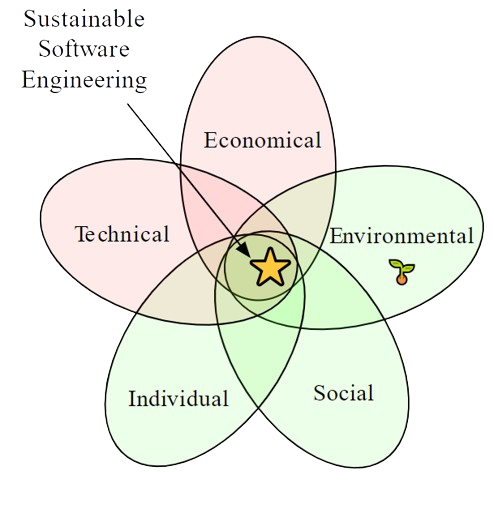
\includegraphics[width=0.4\textwidth]{MemoireMaster-NestorSkoczylas/figures/Sustainable Software Engineering.png}
    \caption{Schéma illustrant la durabilité dans le génie logiciel}
    \label{fig:durabilite-geni-logiciel}
\end{figure}

C'est dans ce contexte que s'inscrit le travail de ce mémoire, qui vise à explorer les différentes facettes de l'ingénierie logicielle durable.

%%%%%%%%%%%%%%%%%%%%%%%%%%%%%%%%%%%% SECTION 2

\section{Description du projet}
\label{sec:Ch0.2}
Ce travail de recherche s'appuie sur une approche interdisciplinaire qui combine des éléments de génie logiciel, de durabilité environnementale et de sciences sociales. 
Il vise à répondre à la questions suivante :
\begin{quote}
    
    \textit{Comment incorporer les principes de développement durable et écologique dans le processus de développement de logiciels en vue de créer des applications plus respectueuses de l'environnement ?}
    
\end{quote}

Cette proposition s'inscrit dans le cadre d'un projet plus large visant à réduire l'impact environnemental des logiciels, qui comprend plusieurs initiatives, notamment l'élaboration de lignes directrices pour l'éco-conception logicielle et la création d'un outil de mesure de l'empreinte carbone des logiciels.

%%%%%%%%%%%%%%%%%%%%%%%%%%%%%%%%%%%% SECTION 3

\section{Objectifs}
\label{sub:Ch0.3}
L'objectif principal de ce mémoire est d'explorer en profondeur les dimensions cruciales de l'ingénierie logicielle durable, mettant en lumière les défis, les opportunités, et les solutions envisageables dans ce domaine. Cette recherche aspire spécifiquement à :
\begin{itemize}
     \item Examiner de manière approfondie l'intégration efficace de la durabilité dans le processus de développement logiciel en vue de réduire son impact environnemental.
     \item Analyser l'influence des pratiques individuelles des ingénieurs logiciels sur la durabilité des produits logiciels résultants.
     \item Investiguer les pratiques durables à l'échelle globale, aussi bien au sein des projets logiciels qu'au sein des équipes de développement, tout en explorant leur cohérence avec les stratégies de la \acrfull{rse}.
\end{itemize}

Chacun de ces objectifs revêt une importance pour éclairer et contribuer à la recherche en ingénierie logicielle durable, en offrant des perspectives novatrices et des solutions concrètes.

%%%%%%%%%%%%%%%%%%%%%%%%%%%%%%%%%%%% SECTION 4
\section{Organisation du rapport}
\label{sec:Ch0.4}
Ce mémoire se compose de trois chapitres, chacun explorant un aspect distinct de la recherche sur l'ingénierie logicielle durable.

\paragraph{Chapitre \ref{mesure} : Mesure de la Durabilité dans le Développement Logiciel}
Ce chapitre examine comment évaluer et quantifier la durabilité des logiciels. Il explore d'abord la conception d'un modèle de mesure complet intégrant la durabilité dans l'évaluation des performances des projets logiciels (Section~\ref{sec:mesure-durabilite}). En suite, il analyse les approches existantes pour la pratique durable du génie logiciel, les classifiant et les évaluant dans un contexte en constante évolution (Section~\ref{sec:approches-durables}). Enfin, il examine les différentes dimensions de la durabilité conceptualisées dans la littérature académique en génie logiciel (Section~\ref{sec:dimensions-durabilite}).

\paragraph{Chapitre \ref{pratique-durabilite} : Pratiques Individuelles des Ingénieurs Logiciels et Durabilité}
Ce chapitre se concentre sur l'influence des pratiques individuelles des ingénieurs logiciels sur la durabilité des logiciels. Il explore d'abord l'impact des facteurs humains dans la conception de logiciels respectueux de l'environnement (Section~\ref{sec:pratiques-individuelles}). Ensuite, il propose des méthodes pour mesurer et améliorer la durabilité des logiciels du point de vue des pratiques individuelles des ingénieurs (Section~\ref{sec:mesure-amelioration}). Enfin, il examine comment le comportement des utilisateurs peut contribuer à la durabilité des logiciels, en soulignant l'importance de la sensibilisation et des retours d'information (Section~\ref{sec:comportement-utilisateurs}).

\paragraph{Chapitre \ref{pratique-globale} : Pratiques Durables au Niveau Global}
Ce chapitre explore les pratiques durables à l'échelle des projets et des organisations. Il examine d'abord la mise en œuvre de pratiques durables au niveau des projets logiciels, en s'appuyant sur les modèles et les outils disponibles pour évaluer et améliorer la durabilité à l'échelle du projet (Section~\ref{sec:pratiques-projets}). Ensuite, il explore comment une équipe de développement peut adopter des pratiques durables au quotidien, en identifiant les initiatives qui peuvent être mises en place pour encourager la durabilité au sein de l'équipe (Section~\ref{sec:pratiques-equipe}). Enfin, il examine comment la stratégie de \acrshort{rse} peut être alignée avec les objectifs de durabilité dans le développement logiciel, tout en abordant les avantages et les défis de l'incorporation de la durabilité dans la culture d'entreprise (Section~\ref{sec:rse-durabilite}).


Chaque chapitre est divisé en sections distinctes, chacune se concentrant sur un aspect précis du sujet. Cette structure permet une exploration approfondie de chaque thème tout en facilitant la navigation à travers le mémoire.

\section{Définition de la Durabilité}
La durabilité, la capacité à répondre \emph{« aux besoins du présent sans compromettre la capacité des générations futures à répondre aux leurs. »}~\cite{Brundtland87} 
Cette vision holistique englobe la notion de responsabilité envers l'environnement, la société, et l'économie, établissant ainsi un équilibre délicat entre les impératifs actuels et la préservation des ressources pour les générations à venir.


Dans le contexte de l'ingénierie logicielle, la durabilité va au-delà de la simple efficacité énergétique des logiciels. Elle englobe la minimisation de l'empreinte carbone, la gestion judicieuse des ressources, la prise en compte des dimensions sociales dans le processus de développement, et la création de solutions technologiques qui favorisent un équilibre harmonieux avec l'écosystème. Ainsi, définir la durabilité dans le contexte du développement logiciel revient à intégrer des principes écologiques, sociaux, et économiques au cœur même du processus de création de logiciels.


En explorant la durabilité dans le domaine du génie logiciel, ce mémoire s'engage à décortiquer ces dimensions multiples. L'analyse approfondie des pratiques individuelles des ingénieurs, la mesure de la durabilité au niveau des projets, et l'examen des implications de la \acrshort{rse} dans le développement logiciel, tous convergent vers une compréhension globale et nuancée de la durabilité dans le contexte des technologies de l'information.


Ainsi, tout au long de cette recherche, la notion de durabilité servira de fil conducteur, guidant l'exploration des défis, des opportunités, et des solutions pour forger un avenir logiciel véritablement durable. En définissant la durabilité dans ce contexte spécifique, ce mémoire aspire à contribuer à l'évolution de l'ingénierie logicielle vers des pratiques plus respectueuses de l'environnement, socialement responsables, et économiquement viables.
% Chapter 1
\chapter{Mesure de la Durabilité dans le Développement Logiciel}	%The main chapter title
\label{mesure}
%%%%%%%%%%%%%%%%%%%%%%%%%%%%%%%%%%%%

Alors que la révolution technologique bat son plein, le génie logiciel se retrouve à la croisée des chemins en matière de durabilité. Ce premier chapitre explore l'intégration de la durabilité dans le développement logiciel, en soulignant les défis, les opportunités et les solutions qui se présentent à nous.


Divisé en trois parties distinctes, ce chapitre examine les aspects clés de la mesure de la durabilité dans le développement logiciel. La première section se concentre sur la conception d'un modèle de mesure complet capable d'évaluer la performance et la durabilité des projets logiciels (Section~\ref{sec:mesure-durabilite}). La deuxième section explore l'état de l'art des approches durables dans le domaine du génie logiciel, en les classifiant et en les évaluant dans un contexte en constante évolution (Section~\ref{sec:approches-durables}). La dernière section analyse les différentes dimensions de la durabilité conceptualisées dans la littérature académique en génie logiciel (Section~\ref{sec:dimensions-durabilite}).

%%%%%%%%%%%%%%%%%%%%%%%%%%%%%%%%%%%%

\section{Modèle de Mesure de la Performance et de Durabilité}\label{sec:mesure-durabilite}

%%%%%%%%%%%%%%%%%%%%%%%%%%%%%%%%%%%%

La mesure de la durabilité est au cœur de notre réflexion sur le génie logiciel durable. 
Pour comprendre comment intégrer efficacement la durabilité dans l'évaluation des performances des projets logiciels, nous débutons en explorant la création d'un modèle de mesure de la performance et de durabilité. Il représente un défi complexe qui nécessite une approche nuancée et multidimensionnelle. 
Plusieurs recherches ont offert des perspectives variées sur cette question cruciale.

\subsection{Approche et critères de mesure}
Le concept de logiciel vert, qui englobe les logiciels respectueux de l'environnement et économes en ressources, est de plus en plus présent dans le paysage contemporain du développement logiciel. Selon les auteurs du journal The GREENSOFT Model, \emph{« producing ecologically sound, resource and energy efficient software is also an issue nowadays »}~\cite{GreenSoftModel}. Cependant, la mesure et l'évaluation de la durabilité des processus de développement de logiciels et des produits logiciels qui en résultent restent un défi.


Pour répondre à ce défi, ces mêmes auteurs proposent \emph{« Appropriate criteria and metrics may comprise models for the measurement of software quality, procedure models for software development, as well as methods borrowed from LCA. Here, we distinguish direct criteria and metrics (related to first-order effects) from those which indirectly concern sustainability (related to second- and third-order effects) »}~\cite{GreenSoftModel}. Ainsi, il est décisif de disposer de cadres globaux qui prennent en compte d'une part les mesures directes et quantifiables de la consommation de ressources et des économies d'énergie, d'autre part les effets indirects sur la durabilité à long terme.


De plus, la prévalence des discussions sur l'efficacité énergétique au sein de la communauté des chercheurs suggère une prise de conscience croissante de l'impact environnemental du développement de logiciels. Dans l'article Green and Sustainable Software Engineering, il est indiqué que \emph{« Several approaches discussed efficiency in terms of energy consumption. This evidence may indicate the need to consider energy efficiency as an important quality attribute when designing systems architectures »}~\cite{GreenSustainableEngMapping}. Il est donc important d'intégrer des considérations de durabilité tout au long du cycle de vie du développement logiciel, de la conception et de l'architecture à la mise en œuvre et à la maintenance.


Enfin, en adoptant une approche multidimensionnelle et des critères de mesure rigoureux, l'industrie du développement logiciel peut s'efforcer de créer des logiciels non seulement fonctionnels et fiables, mais aussi écologiquement responsables et contribuant à un avenir durable. Il existe déjà des efforts importants pour atteindre cet objectif : \emph{« We observed that 56\% of the primary studies proposed means to achieve the energy efficiency of the software in terms of consumption and energy savings »}~\cite{GreenSustainableEngMapping}.

\begin{figure}[H]
    \centering
    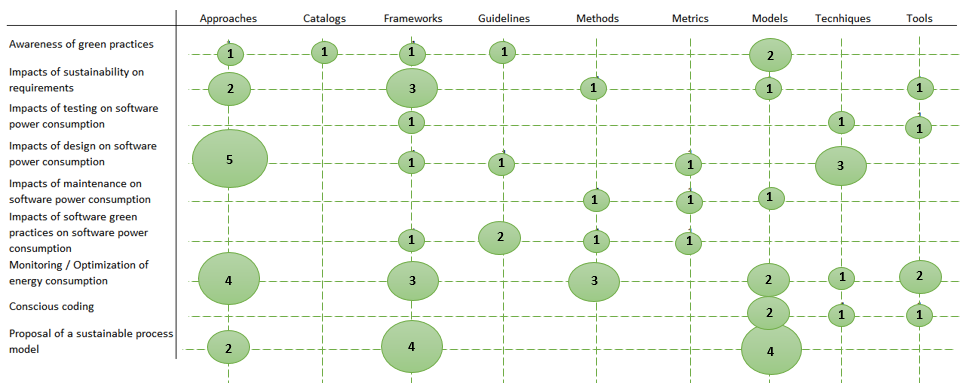
\includegraphics[width=1\textwidth]{MemoireMaster-NestorSkoczylas/figures/Répartition des études primaires selon les modèles de produits et processus proposés.png}
    \caption{Répartition des études primaires selon les modèles de produits et processus proposés}
    \label{fig:repartition-etudes-primaires}
\end{figure}

Comme le montre la Figure \ref{fig:repartition-etudes-primaires}, la plupart des études se concentrent sur les modèles de produits (approches, frameworks, etc.) pour le développement logiciel durable, tandis que les modèles de processus (13\%) sont moins étudiés. Parmi les rares modèles de processus proposés, seulement deux s'appuient sur des normes de qualité SE traditionnelles.

Ce manque de modèles de processus durables souligne la nécessité d'investir davantage dans ce domaine pour atteindre l'objectif d'un développement logiciel plus écologique. En effet, les modèles de processus guident les développeurs dans la création de logiciels économes en énergie et respectueux de l'environnement.

% Approach and measurement criteria
%~\cite{GreenSoftModel}	"Appropriate criteria and metrics may comprise models for the measurement of software quality, procedure models for software development, as well as methods borrowed from LCA. Here, we distinguish direct criteria and metrics (related to first-order effects) from those which indirectly concern sustainability (related to second- and third-order effects)."
%~\cite{GreenSoftModel}	"Appropriate criteria and metrics may comprise models for the measurement of software quality, procedure models for software development, as well as methods borrowed from LCA. Here, we distinguish direct criteria and metrics (related to first-order effects) from those which indirectly concern sustainability (related to second- and third-order effects)."
%~\cite{GreenSustainableEngMapping} "We observed that 56\% of the primary studies proposed means to achieve the energy efficiency of the software in terms of consumption and energy savings"
%~\cite{GreenSustainableEngMapping} "Several approaches discussed efficiency in terms of energy consumption. This evidence may indicate the need to consider energy efficiency as an important quality attribute when designing systems architectures."

\subsection{Intégrer des pratiques écologiques dans le \acrfull{sdlc}}
L'intégration efficiente de pratiques écologiques dans le \acrshort{sdlc} constitue un élément crucial pour atteindre un développement durable des logiciels. Bien que diverses approches et cadres soient disponibles, comme le souligne l'article~\cite{GreenSoftModel} : \emph{« Besides reflecting the proposed life cycle of a software product, there are further methods that support software architects, designers, and developers in producing green and sustainable software applications. »} Toutefois, des défis persistent pour intégrer harmonieusement ces pratiques avec les processus de développement existants.


Un aspect important à considérer réside dans la distinction entre les pratiques écologiques et les activités traditionnelles du \acrshort{sdlc}. L'article~\cite{GreenAgileMethods} affirme que : \emph{« The Sustainability Retrospective and the Sprint Retrospectives should not be combined, because they have a different timely position regarding the process flow and the focus »}, soulignant ainsi la nécessité de disposer de mécanismes distincts pour évaluer et améliorer la durabilité, en parallèle aux rétrospectives régulières du cycle de développement.


Selon l'article~\cite{GreenSustainableEngMapping} : \emph{« It was also possible to understand how sustainability has been addressed in the SLDC. The SMS shows that approaches and frameworks are mainly focused on the requirements and design phases. »} Cependant, la recherche actuelle suggère que la mise en œuvre des pratiques écologiques se limite souvent à ces premières étapes du \acrshort{sdlc}. Ce constat implique un besoin potentiel d'intégration plus large des aspects écologiques tout au long du cycle de développement, y compris les phases de mise en œuvre, de test, de déploiement et de maintenance.


Afin d'assurer une approche holistique et efficace pour atteindre les objectifs de développement de logiciels écologiques, une analyse approfondie des différences temporelles et fonctionnelles entre les pratiques écologiques et les activités traditionnelles du \acrshort{sdlc} s'avère nécessaire. En élargissant le champ d'intégration au-delà des phases initiales du développement, l'industrie du développement de logiciels peut garantir une approche plus globale et plus efficace pour atteindre les objectifs de développement de logiciels écologiques.

% Integration with the Software Development Life Cycle (SDLC)
%~\cite{GreenAgileMethods}	"The Sustainability Retrospective and the Sprint Retrospectives should not be combined, because they have a different timely position regarding the process flow and the focus."
%~\cite{GreenSoftModel}	"Besides reflecting the proposed life cycle of a software product, there are further methods that support software architects, designers, and developers in producing green and sustainable software applications."
%~\cite{GreenSustainableEngMapping} "It was also possible to understand how sustainability has been addressed in the SLDC. The SMS shows that approaches and frameworks are mainly focused on the requirements and design phases."

\subsection{Recherche et orientation futures}
Pour faire progresser le domaine de l'ingénierie logicielle écologique, une approche à multiples facettes est nécessaire, combinant recherche empirique et exploration des orientations futures. L'étude des perspectives des praticiens est essentielle pour comprendre les pratiques actuelles et identifier les domaines à améliorer. Selon~\cite{EmpiricalStudy} : \emph{« an analysis of the collected data that identifies practitioners’ perspectives on green software engineering throughout the software development process. »}


En s'appuyant sur cette base, des recherches plus approfondies peuvent contextualiser les connaissances existantes avec de nouveaux résultats.~\cite{EmpiricalStudy} propose \emph{« a discussion that contextualizes the state-of-the-art in green software engineering research with respect to the study’s findings, and suggests, for each stage of the software development process, directions for future green software engineering research. »} Cette approche synergique comble le fossé entre les connaissances théoriques et l'application pratique, conduisant à des pratiques de développement de logiciels écologiques plus efficaces et plus faciles à mettre en œuvre.


Il est important de souligner la nécessité d'un développement et d'une amélioration continus des différents aspects de l'ingénierie logicielle écologique.~\cite{GreenSustainableEngMapping} appuie cette idée en affirmant que : \emph{« There are several directions to follow towards establishing and improving Green SE practice, in particular in order to provide the SE practice with green and sustainability-aware processes, tools and methods. »} Ces orientations incluent la création de nouveaux outils et méthodologies, l'amélioration des processus existants et le développement de ressources éducatives pour doter les professionnels du logiciel des compétences et connaissances nécessaires pour concevoir, développer et maintenir des solutions logicielles durables.


La recherche empirique associé à une vision prospective, permet de tracer la voie vers un avenir où le développement de logiciels n'est pas seulement innovant et fonctionnel, mais également respectueux de l'environnement tout en contribuant à un avenir durable.

% Recherche et orientations futures
%~\cite{EmpiricalStudy}	"An analysis of the collected data that identifies practitioners’ perspectives on green software engineering throughout the software development process."
%~\cite{EmpiricalStudy}	"A discussion that contextualizes the state-of-the-art in green software engineering research with respect to the study’s findings, and suggests, for each stage of the software development process, directions for future green software engineering research."
%~\cite{GreenSustainableEngMapping} "There are several directions to follow towards establishing and improving Green SE practice, in particular in order to provide the SE practice with green and sustainability-aware processes, tools and methods."

\subsection{Modèles et théories existants}
Comprendre les modèles et théories existants est crucial pour enrichir la base de connaissances actuelle en matière de développement de logiciels écologiques. Ces modèles offrent des cadres pour conceptualiser la relation entre le développement de logiciels et la durabilité.


Le schéma illustrant la durabilité dans le génie logiciel (\ref{fig:durabilite-geni-logiciel}) présente une synthèse des principaux modèles et théories en matière de développement de logiciels durables. On peut y observer les différentes dimensions de la durabilité, ainsi que les relations entre elles.


Parmi ces modèles, le modèle GREENSOFT se distingue en mettant l'accent sur l'importance des critères et des mesures de durabilité (dimension économique de la figure \ref{fig:durabilite-geni-logiciel}).

Selon \cite{GreenSoftModel} : \emph{« The second part of the GREENSOFT Model is called Sustainability Criteria and Metrics. It covers common metrics and criteria for the measurement of software quality and it allows a classification of criteria and metrics for evaluating a software product’s sustainability. »} Il offre une approche structurée pour évaluer l'impact environnemental des produits logiciel.

\begin{figure}[H]
    \centering
    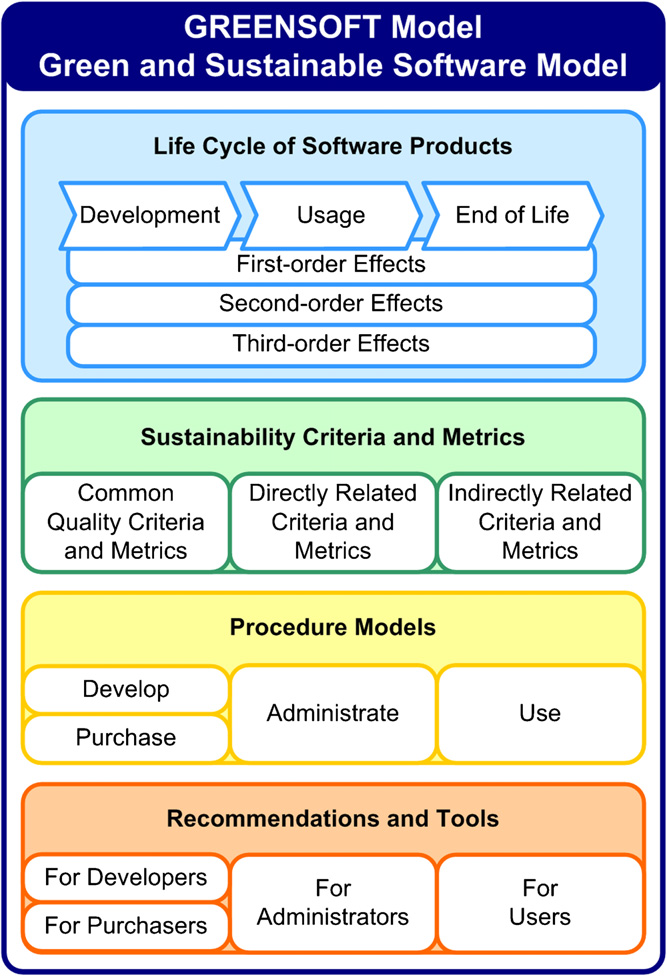
\includegraphics[width=0.4\textwidth]{MemoireMaster-NestorSkoczylas/figures/greensoft_model.png}
    \caption{Le modèle GREENSOFT}
    \label{fig:greensoft-model}
\end{figure}

La figure ci-dessus (\ref{fig:greensoft-model}) présente le modèle GREENSOFT. Le cycle de vie des produits logiciels est représenté au centre de la figure. Les trois phases du cycle de vie (développement, utilisation et fin de vie) sont représentées par des rectangles. Les autres éléments du modèle GREENSOFT (critères et métriques de durabilité, modèles de procédure, recommandations et outils) sont représentés autour du cycle de vie.

La théorie de la stratification durable, quant à elle, propose une perspective nuancée sur la relation entre le développement de logiciels et la durabilité (dimensions sociale et environnementale de la \ref{fig:durabilite-geni-logiciel}). Cette théorie, telle qu’elle est citée dans~\cite{SustainableStratifiedTheory}, \emph{« explain how sustainability relates to software development based on existing qualitative research and to provide a more nuanced view of the stratified and multisystemic nature of sustainability according to our observations from the meta-synthesis. »} En reconnaissant la nature complexe et interconnectée de la durabilité, cette théorie encourage une approche globale du développement de logiciels écologiques.


De plus, la théorie de la stratification durable met en évidence l'interdépendance des processus et des produits logiciels. Selon~\cite{SustainableStratifiedTheory} : \emph{« The model separates the software process from the software product to illustrate that sustainability is a property of both, and while the nature of the software development process affects the resulting software system, a sustainable process does not guarantee a sustainable product or vice versa. »} Cela souligne la nécessité de considérer les deux aspects en tandem lors du développement de logiciels durables.


En étudiant et en évaluant de manière critique les modèles et théories existants, la communauté des développeurs de logiciels peut acquérir des connaissances précieuses sur les complexités et les interrelations inhérentes à ce domaine. Ces connaissances peuvent ensuite servir de base à de nouveaux efforts de recherche et de développement, ouvrant ainsi la voie à un avenir plus durable en matière de développement de logiciels.

% Modèles et théories existants
%~\cite{GreenSoftModel}	"The second part of the GREENSOFT Model is called Sustainability Criteria and Metrics. It covers common metrics and criteria for the measurement of software quality [43] and it allows a classification of criteria and metrics for evaluating a software product’s sustainability."
%~\cite{SustainableStratifiedTheory} "The goal of this model is to explain how sustainability relates to software development based on existing qualitative research and to provide a more nuanced view of the stratified and multisystemic nature of sustainability according to our observations from the meta-synthesis."
%~\cite{SustainableStratifiedTheory} "The model separates the software process from the software product to illustrate that sustainability is a property of both, and while the nature of the software development process affects the resulting software system, a sustainable process does not guarantee a sustainable product or vice versa."

\paragraph{}
En guise de conclusion, l'élaboration d'un modèle de mesure de la performance et de la durabilité constitue un élément fondamental pour l'ingénierie logicielle durable. Cette tâche ardue nécessite une approche multidimensionnelle qui prend en compte divers aspects, notamment :

\begin{itemize}
    \item Critères et mesures de durabilité : Définir des critères précis et des indicateurs pertinents pour évaluer l'impact environnemental des logiciels, en se basant sur des modèles existants tels que GREENSOFT.
    \item Intégration des pratiques écologiques : Concevoir des processus et des outils favorisant l'intégration harmonieuse de pratiques écologiques tout au long du \acrshort{sdlc}, en dépassant les phases initiales.
    \item Recherche et orientation futures : Promouvoir la recherche empirique et l'exploration de nouvelles orientations pour combler le fossé entre la théorie et la pratique, et améliorer continuellement les processus, outils et méthodes de développement de logiciels écologiques.
    \item Modèles et théories existants : Exploiter les connaissances et les perspectives offertes par des modèles comme GREENSOFT et la théorie de la stratification durable pour mieux appréhender les complexités et les interrelations inhérentes à la durabilité dans le développement de logiciels.
\end{itemize}

En abordant ces défis de manière holistique et proactive, l'industrie du développement logiciel peut s'orienter vers un avenir où la performance et la durabilité ne sont plus des concepts mutuellement exclusifs, mais plutôt des piliers complémentaires d'une ingénierie logicielle responsable et respectueuse de l'environnement.

%%%%%%%%%%%%%%%%%%%%%%%%%%%%%%%%%%%%

\section{État de l'Art des Approches Durables dans le Génie Logiciel}\label{sec:approches-durables}

%%%%%%%%%%%%%%%%%%%%%%%%%%%%%%%%%%%%
Reprenons l'exploration de l'ingénierie logicielle durable, un domaine qui requiert une compréhension approfondie des approches existantes. Dans cette section, nous nous pencherons sur l'état de l'art des approches durables dans le génie logiciel. La découverte de ces approches nous permet d'identifier les meilleures pratiques et les lacunes à combler dans notre quête de logiciels plus respectueux de l'environnement.

\subsection{Définir et définir le champ d'application de l'ingénierie logicielle verte}
L'ingénierie logicielle écologique constitue un domaine émergent dans le paysage du développement logiciel, visant à instaurer des pratiques durables et respectueuses de l'environnement tout au long du cycle de vie du développement logiciel. Comme le souligne l'article~\cite{GreenSoftModel} : \emph{« Starting from our definitions, Green and Sustainable Software Engineering produces Green and Sustainable Software in an environmental-friendly and sustainable way. »} Cette définition met en lumière l'approche holistique de l'ingénierie logicielle verte, qui englobe non seulement la création de produits logiciels durables, mais aussi la mise en œuvre de processus de développement respectueux de l'environnement.


Il est cependant essentiel de prendre conscience de la complexité inhérente à la réalisation d'une durabilité complète dans le cadre du développement de logiciels. L'article~\cite{GreenSoftModel} précise : \emph{« Thus, there is no guarantee that the resulting software products are more sustainable than they would have been without applying this process. »} Cette nécessité d'une recherche et d'un développement continus pour affiner les pratiques existantes et élaborer des solutions innovantes contribuent de manière avérée aux objectifs globaux de durabilité.


La reconnaissance croissante de ce besoin est manifeste dans l'article~\cite{EmpiricalStudy} : \emph{« The research community has not been blind to these changes and, as a result, green software engineering—the process of helping practitioners (architects, developers, testers, managers, etc.) write more energy efficient applications—is increasingly targeted as an important problem area by software engineering researchers. »} Cette prise de conscience met en évidence l'importance grandissante accordée à l'ingénierie logicielle écologique au sein de la communauté des chercheurs, avec un accent particulier sur le développement de stratégies et d'outils pour aider les praticiens à optimiser l'efficacité énergétique des applications logicielles. L'article poursuit en mentionnant \emph{« the major findings and implications from the collected data contextualize existing green software engineering research and suggest directions for researchers aiming to develop strategies and tools to help practitioners improve the energy usage of their applications »}~\cite{EmpiricalStudy}.


Par ailleurs, l'émergence de l'ingénierie logicielle verte en tant que discipline distincte au sein du secteur des technologies de l'information, comme l'indique l'article~\cite{IntegrationSustainabilityMetrics} sur \emph{« implementing these principles within the information technology sector has led to the emergence of a new discipline, green software engineering, which focuses on writing energy-efficient software. »} Ce domaine est de plus en plus important et reconnu pour relever les défis environnementaux associés au développement de logiciels.


En définissant le champ d'application de l'ingénierie logicielle verte, en reconnaissant ses complexités inhérentes et en prenant en compte les efforts de recherche croissants, la communauté du développement logiciel peut collectivement œuvrer à l'établissement de pratiques durables et contribuer à un avenir plus respectueux de l'environnement.

% Définition et portée du génie logiciel vert
%~\cite{GreenSoftModel}	"Starting from our definitions, Green and Sustainable Software Engineering produces Green and Sustainable Software in an environmental-friendly and sustainable way."
%~\cite{GreenSoftModel}	"FIGURE 'Example for enhancing software development processes that fits into the procedure model part “Develop”'"
%~\cite{GreenSoftModel}	"Thus, there is no guarantee that the resulting software products are more sustainable than they would have been without applying this process."
%~\cite{EmpiricalStudy}	"The research community has not been blind to these changes and, as a result, green software engineering—the process of helping practitioners (architects, developers, testers, managers, etc.) write more energy efficient applications—is increasingly targeted as an important problem area by software engineering researchers."
%~\cite{EmpiricalStudy}	"The major findings and implications from the collected data contextualize existing green software engineering research and suggest directions for researchers aiming to develop strategies and tools to help practitioners improve the energy usage of their applications."
%~\cite{IntegrationSustainabilityMetrics} "Implementing these principles within the information technology sector has led to the emergence of a new discipline, green software engineering, which focuses on writing energy-efficient software."

\subsection{Classification des approches écologiques en matière de génie logiciel}
L'ingénierie logicielle écologique englobe une multitude d'approches, chacune ayant ses propres forces et domaines d'intérêt. Il est essentiel de comprendre ces classifications pour sélectionner l'approche la plus efficace pour un projet ou un contexte spécifique.


Une étude~\cite{GreenSustainableEngMapping} souligne le défi que représente un système de classification unifié : \emph{« We also noticed a lack of conceptual standards to characterize the contribution types in SE. This can be evidenced, which use the terms “SE topics", “approaches" and “sub-domains" as synonyms for such a definition »}. Ce manque de normalisation caractérise la nature évolutive de l'ingénierie logicielle écologique et la nécessité de poursuivre les efforts pour établir un système de classification clair et cohérent.


Malgré les difficultés, la recherche montre que l'accent est mis sur l'intégration de pratiques durables tout au long du \acrshort{sdlc}, comme le montre la Figure \ref{fig:repartition-etudes-primaires}. Comme cité dans~\cite{GreenSustainableEngMapping} : \emph{« Regarding sustainable practices throughout the SDLC, 68\% studies analyze the impacts and implications of applying sustainable practices to traditional software activities »}. Cette constatation indique que l'on reconnaît de plus en plus l'importance d'intégrer des considérations de durabilité à tous les stades du développement de logiciels, non pas comme des efforts isolés, mais comme une approche intégrée et holistique. Cette concentration sur l'intégration de la durabilité dans le SDLC est encourageante, car elle montre que l'industrie reconnaît l'importance de créer des logiciels écologiquement responsables.

En reconnaissant la diversité des approches d'ingénierie logicielle écologique et en reconnaissant les efforts en cours pour établir un système de classification unifié, la communauté du développement de logiciels peut continuer à affiner et à améliorer ses pratiques, conduisant finalement à un avenir plus durable pour le développement de logiciels.

% Classification des approches de génie logiciel vert
%~\cite{GreenSustainableEngMapping} "We also noticed a lack of conceptual standards to characterize the contribution types in SE. This can be evidenced in [ 2 , 11 , 12], which use the terms “SE topics", “approaches" and “sub-domains" as synonyms for such a definition"
%~\cite{GreenSustainableEngMapping} "Regarding sustainable practices throughout the SDLC, 68\% studies analyze the impacts and implications of applying sustainable practices to traditional software activities"

\subsection{Évaluer les progrès et tracer l'avenir de l'ingénierie logicielle écologique}
L'évaluation de l'efficacité des pratiques d'ingénierie logicielle écologique et l'identification des orientations futures sont cruciales pour l'amélioration continue et le progrès dans ce domaine.


Une approche prometteuse consiste à élargir la portée des considérations relatives au \acrshort{sdlc} pour englober les aspects écologiques, sociaux et environnementaux, comme le souligne la citation de~\cite{GreenAgileMethods} : \emph{« The life cycle of software products considers ecological, social, and environmental aspects of a software product over its whole life. »}. Cette approche holistique garantit que la durabilité n'est pas considérée comme une préoccupation isolée, mais qu'elle est intégrée dans l'ensemble du processus de développement de logiciels.


D'autre part, l'article~\cite{GreenAgileMethods} met en évidence la faisabilité de l'amélioration continue : \emph{« The approach presented shows that it is feasible to continuously improve software projects regarding sustainability issues by measuring a set of metrics repeatedly over several iterations »}, reflétant ainsi l'importance d'établir et d'utiliser des mesures pour quantifier les progrès et identifier les domaines à optimiser.


Au-delà de l'évaluation, des efforts de recherche sont en cours pour développer des outils et des modèles qui soutiennent le développement de logiciels écologiques. Comme cité dans~\cite{EmpiricalStudy} : \emph{« There is also research focused on both developing tools to help developers examine/improve the energy usage of their applications, and on models to support the green software development process. »}. Ces avancées fourniront aux praticiens du logiciel les ressources et les conseils nécessaires pour mettre en œuvre des pratiques écologiques de manière efficace.


L'article~\cite{GreenSustainableEngMapping} insiste davantage sur la nécessité d'établir et d'améliorer les pratiques d'ingénierie logicielle écologique : \emph{« There are several directions to follow towards establishing and improving Green SE practice, in particular in order to provide the SE practice with green and sustainability-aware processes, tools and methods »}, faisant ressortir l'importance de la recherche et du développement continus pour affiner les pratiques existantes et créer de nouvelles solutions qui répondent aux défis évolutifs de l'ingénierie logicielle écologique.


Enfin, la théorie de la stratification durable offre des perspectives précieuses tant pour les chercheurs que pour les praticiens. Cette phrase provenant de~\cite{SustainableStratifiedTheory}, met l'accent sur la nature participative de la durabilité : \emph{« Meanwhile, to approach sustainability as a participatory process, the model implies asking which dimensions, layers and subsystems the participants should come from, and whether they are participating in the design of the process or product »}. Tout en encourageant une approche collaborative où toutes les parties prenantes peuvent contribuer au développement et à la mise en œuvre de solutions logicielles durables.


En combinant une évaluation rigoureuse, des efforts d'amélioration continue et une approche collaborative, la communauté des développeurs de logiciels peut relever les défis et saisir les opportunités de l'ingénierie logicielle écologique, contribuant ainsi à un avenir plus durable pour l'ensemble du secteur.

% Evaluation and Future Directions
%~\cite{GreenAgileMethods}	"The life cycle of software products considers ecological, social, and environmental aspects of a software product over its whole life."
%~\cite{GreenAgileMethods}	"The approach presented shows that it is feasible to continuously improve software projects regarding sustainability issues by measuring a set of metrics repeatedly over several iterations."
%~\cite{EmpiricalStudy}	"There is also research focused on both developing tools to help developers examine/improve the energy usage of their applications, and on models to support the green software development process."
%~\cite{GreenSustainableEngMapping}	"There are several directions to follow towards establishing and improving Green SE practice, in particular in order to provide the SE practice with green and sustainability-aware processes, tools and methods"
%~\cite{SustainableStratifiedTheory} "The proposed model has important implications for both researchers assessing sustainability and practitioners approaching sustainability as a participatory process"
%~\cite{SustainableStratifiedTheory} "Meanwhile, to approach sustainability as a participatory process, the model implies asking which dimensions, layers and subsystems the participants should come from, and whether they are participating in the design of the process or product"

\paragraph{}
L'ingénierie logicielle écologique est un domaine en plein essor qui s'attaque aux défis environnementaux et sociaux du développement de logiciels. Cette section a exploré l'état de l'art des approches durables dans le génie logiciel, en se concentrant sur trois aspects clés :

\begin{itemize}
    \item Définir et délimiter le champ d'application de l'ingénierie logicielle verte : L'ingénierie logicielle verte vise à créer des logiciels durables et à mettre en œuvre des processus de développement respectueux de l'environnement. Il est important de reconnaître la complexité de la durabilité et de poursuivre la recherche et le développement pour affiner les pratiques existantes.
    \item Classification des approches écologiques en matière de génie logiciel : Il existe une variété d'approches d'ingénierie logicielle écologique, chacune ayant ses propres forces et domaines d'intérêt. Un système de classification unifié n'est pas encore en place, mais l'accent est mis sur l'intégration de pratiques durables tout au long du \acrshort{sdlc}.
    \item Évaluer les progrès et tracer l'avenir de l'ingénierie logicielle écologique : L'évaluation des pratiques d'ingénierie logicielle écologique et l'identification des orientations futures sont essentielles pour l'amélioration continue et le progrès dans ce domaine. Des efforts de recherche sont en cours pour développer des outils et des modèles qui soutiennent le développement de logiciels écologiques, et la théorie de la stratification durable offre des perspectives précieuses pour les chercheurs et les praticiens.
\end{itemize}

En conclusion, l'ingénierie logicielle écologique est un domaine dynamique et prometteur qui a le potentiel de transformer l'industrie du logiciel et de contribuer à un avenir plus durable. En combinant une compréhension approfondie des approches existantes, une évaluation rigoureuse et des efforts d'amélioration continue, la communauté des développeurs de logiciels peut relever les défis et saisir les opportunités de l'ingénierie logicielle écologique.

%%%%%%%%%%%%%%%%%%%%%%%%%%%%%%%%%%%%

\section{Application de la Théorie de la Durabilité aux Projets de Développement Logiciel}\label{sec:dimensions-durabilite}

%%%%%%%%%%%%%%%%%%%%%%%%%%%%%%%%%%%%
Les projets de développement logiciel nécessitent une exploration approfondie des fondements théoriques sous-jacents à la théorie de la durabilité. Cette section offre un aperçu des perspectives cruciales qui éclairent notre compréhension de l'ingénierie logicielle durable.

\subsection{Définir et englober la durabilité}
Le concept de durabilité, qui sert de fondement à l'ingénierie logicielle écologique, incarne une approche à multiples facettes visant à répondre aux besoins du présent sans compromettre la capacité des générations futures à répondre aux leurs. Comme l'indique très justement~\cite{IntegrationSustainabilityMetrics} : \emph{« Sustainability emphasizes meeting current needs without compromising the ability of future generations to satisfy their requirements. It consists of three elements: social, economic, and environmental factors »}. Cette définition met en évidence l'interconnexion de ces dimensions, soulignant qu'une véritable durabilité ne peut être atteinte en se concentrant uniquement sur un aspect au détriment des autres.


Dans le contexte du développement de logiciels, la durabilité environnementale occupe souvent le devant de la scène, l'accent étant mis sur la réduction de l'impact environnemental des produits logiciels tout au long de leur cycle de vie. Cela inclut des considérations telles que la consommation d'énergie, l'utilisation des ressources et la production potentielle de déchets électroniques. Cependant, il est essentiel de reconnaître la portée plus large de la durabilité en ce qui concerne l'ingénierie logicielle écologique.


La dimension sociale de la durabilité englobe l'impact du développement de logiciels sur les individus et les communautés. Elle inclut des considérations telles que les pratiques de travail équitables, l'accès équitable à la technologie et le potentiel d'exclusion sociale découlant de la mise en œuvre de nouvelles technologies.


La dimension économique de la durabilité se concentre sur la viabilité économique à long terme des pratiques de développement de logiciels. Elle inclut des considérations telles que l'efficacité des ressources, la rentabilité et le potentiel de création d'emplois associés au développement et au déploiement de solutions logicielles durables.


En reconnaissant la nature multiforme de la durabilité et en intégrant ses différentes dimensions dans le processus de développement de logiciels, le domaine de l'ingénierie logicielle verte peut s'efforcer de créer des solutions holistiques et percutantes qui contribuent à un avenir plus durable pour tous.

% Définition et portée de la durabilité
%~\cite{IntegrationSustainabilityMetrics} "Sustainability emphasizes meeting current needs without compromising the ability of future generations to satisfy their requirements. It consists of three elements: social, economic, and environmental factors."

\subsection{Application des principes de durabilité au génie logiciel}
L'incorporation des principes de durabilité dans le secteur des technologies de l'information a donné naissance à l'ingénierie logicielle verte. Selon~\cite{IntegrationSustainabilityMetrics}, \emph{« Implementing these principles within the information technology sector has led to the emergence of a new discipline, green software engineering, which focuses on writing energy-efficient software. »} Ce nouveau domaine aspire à concevoir des solutions logicielles durables qui non seulement réduisent les impacts négatifs sur l'environnement, mais offrent également des avantages sociétaux et économiques plus étendus.


Quelle est la définition d'un logiciel durable ? D'après~\cite{IntegrationSustainabilityMetrics}, \emph{« the former, referred to as sustainable software, is characterized by its durability, maintainability, and cost-efficiency. In essence, sustainable software entails developing, deploying, and using software that minimizes negative impacts or even generates a positive influence, directly or indirectly, on the economy, society, human beings, and the environment. »} Cette définition souligne la nature holistique des logiciels durables, qui englobent non seulement les facteurs environnementaux, mais aussi les considérations sociales et économiques.


L'application des principes de durabilité dans l'ingénierie logicielle a été abordée sous différents angles, comme le mentionne~\cite{GreenSustainableEngMapping} : \emph{« Several studies have addressed the impact of sustainability in the SE practice, from a range of perspectives. »} Ces recherches posent les fondations de l'élaboration de stratégies et d'outils pratiques pour mettre en œuvre ces principes de manière efficace.


La théorie de la stratification durable~\cite{SustainableStratifiedTheory} met davantage l'accent sur la nature multidimensionnelle de la durabilité dans le développement de logiciels. \emph{« The model depicts four dimensions or pillars of sustainability—environmental, social, economic and technical. All four dimensions apply to software products. »} Cette théorie met en évidence la nécessité de prendre en compte l'interconnexion de ces dimensions et de veiller à ce que les considérations de durabilité soient intégrées à toutes les étapes du cycle de vie du développement logiciel.


En adoptant les principes de l'ingénierie logicielle écologique et en les appliquant à toutes les dimensions de la durabilité, la communauté des développeurs de logiciels peut faire un pas significatif vers la construction d'un avenir plus vert, une ligne de code à la fois.

% Application au génie logiciel
%~\cite{IntegrationSustainabilityMetrics} "Implementing these principles within the information technology sector has led to the emergence of a new discipline, green software engineering, which focuses on writing energy-efficient software."
%~\cite{IntegrationSustainabilityMetrics} "The former, referred to as sustainable software, is characterized by its durability, maintainability, and cost-efficiency. In essence, sustainable software entails developing, deploying, and using software that minimizes negative impacts or even generates a positive influence, directly or indirectly, on the economy, society, human beings, and the environment."
%~\cite{GreenSustainableEngMapping} "Several studies have addressed the impact of sustainability in the SE practice, from a range of perspectives"
%~\cite{SustainableStratifiedTheory} "The model depicts four dimensions or pillars of sustainability—environmental, social, economic and technical. All four dimensions apply to software products."

\subsection{Orientations de la recherche et perspectives d'avenir dans le domaine de l'ingénierie logicielle écologique}
Le domaine en plein essor de l'ingénierie logicielle écologique offre des opportunités passionnantes en matière de recherche et de développement, en vue de façonner un avenir plus durable pour l'industrie du logiciel.


L'intérêt croissant pour ce domaine est évident, comme le souligne~\cite{GreenSustainableEngMapping} : \emph{« The results indicated a growing interest by the SE research community in the Green and Sustainable software domain. »} Cet enthousiasme favorise un environnement collaboratif pour les chercheurs et les praticiens afin de relever les défis et de libérer le potentiel du développement de logiciels verts.


L'un des principaux axes de recherche est l'optimisation de l'efficacité énergétique. La citation de~\cite{GreenSustainableEngMapping} indique : \emph{« This may indicate that researchers expect these three contribution types would promote gains in energy efficiency and, consequently, to obtain more sustainable software products. »} Cela met en évidence les efforts continus pour développer des techniques et des outils innovants qui minimisent l'empreinte environnementale des applications logicielles, comme le montre la figure ci-dessous.

\begin{figure}[H]
    \centering
    \includegraphics[width=0.8\textwidth]{MemoireMaster-NestorSkoczylas/figures/Répartition des articles par type de contribution.png}
    \caption{Répartition des articles par type de contribution}
    \label{fig:repartition-article-type-contribution}
\end{figure}

Cette figure \ref{fig:repartition-article-type-contribution} montre que les chercheurs se concentrent principalement sur les approches (19\%), les frameworks (19\%) et les modèles (16\%) pour améliorer l'efficacité énergétique des logiciels. Cela indique que la recherche se focalise sur le développement de solutions générales et de haut niveau pour la durabilité logicielle. Cette concentration sur les approches, frameworks et modèles montre que la recherche en est encore à ses débuts dans le domaine de l'efficacité énergétique logicielle. Il est nécessaire d'explorer davantage les autres types de contributions, tels que les techniques (8\%), les méthodes (8\%), les outils (7\%), les lignes directrices (5\%), les métriques (4\%) et les catalogues (1\%), pour développer des solutions plus spécifiques et contextuelles.

Toutefois, il est essentiel de reconnaître que la durabilité ne se limite pas à des considérations environnementales. Comme indiqué dans~\cite{SustainableStratifiedTheory} : \emph{« We also found that research focuses heavily on the sustainability of software products (vs. development processes) and ecological (vs. economic and social) sustainability. »} Cette observation souligne la nécessité d'un programme de recherche plus large qui aborde la nature multidimensionnelle de la durabilité dans le cadre du développement de logiciels.


Les futurs efforts de recherche devraient s'efforcer de mettre l'accent de manière équilibrée sur les points suivants :

\begin{itemize}
    \item Les produits logiciels : Explorer les moyens de concevoir, développer et déployer des logiciels avec un impact minimal sur l'environnement, tout en tenant compte de facteurs tels que la maintenabilité et la durabilité.
    \item Les processus de développement : Intégrer les principes de durabilité tout au long du cycle de développement durable, de l'ingénierie des besoins au déploiement et à la maintenance.
    \item Aspects sociaux et économiques : Étudier les implications sociales et économiques potentielles du développement de logiciels verts, telles que la création d'emplois, l'accès équitable à la technologie et la gestion responsable des données.
\end{itemize}


En diversifiant le paysage de la recherche et en adoptant une approche holistique, la communauté des développeurs de logiciels peut continuer à repousser les limites de l'ingénierie logicielle écologique, contribuant ainsi à un avenir plus durable et plus équitable pour tous.

% Axes de recherche et orientations futures
%~\cite{GreenSustainableEngMapping} "The results indicated a growing interest by the SE research community in the Green and Sustainable software domain"
%~\cite{GreenSustainableEngMapping} "This may indicate that researchers expect these three contribution types would promote gains in energy efficiency and, consequently, to obtain more sustainable software products"
%~\cite{SustainableStratifiedTheory} "We also found that research focuses heavily on the sustainability of software products (vs. development processes) and ecological (vs. economic and social) sustainability."

\paragraph{}
L'application de la théorie de la durabilité aux projets de développement logiciel est une étape cruciale pour construire un avenir plus respectueux de l'environnement et plus juste. Le concept de durabilité englobe les dimensions sociales, économiques et environnementales, et l'ingénierie logicielle écologique vise à créer des solutions logicielles durables qui minimisent les impacts négatifs sur l'environnement et offrent des avantages sociétaux et économiques. La théorie de la stratification durable met en évidence la nature multidimensionnelle de la durabilité dans le développement de logiciels, et le domaine de l'ingénierie logicielle écologique est en pleine croissance, offrant des opportunités de recherche et de développement passionnantes. Les efforts de recherche futurs devraient s'efforcer de mettre l'accent sur les produits logiciels, les processus de développement et les aspects sociaux et économiques de la durabilité. En conclusion, l'ingénierie logicielle écologique est un domaine dynamique et prometteur qui offre de nombreuses opportunités pour faire progresser la durabilité dans le secteur des technologies de l'information.

%%%%%%%%%%%%%%%%%%%%%%%%%%%%%%%%%%%%

\paragraph{Conclusion}
Ce chapitre a exploré les défis et les opportunités liés à la mesure de la durabilité dans le développement logiciel. En conclusion, il est crucial de retenir les points suivants :

\begin{enumerate}
    \item Importance de la Mesure : La mesure de la durabilité est essentielle pour évaluer l'impact environnemental, social et économique des logiciels. Cette évaluation permet de suivre les progrès, d'identifier les points d'amélioration et de prendre des décisions éclairées concernant les pratiques de développement.
    \item Complexité de la Mesure : La durabilité est un concept multidimensionnel, ce qui rend sa mesure complexe. Il n'existe pas d'indicateur unique et universel, et différents aspects doivent être pris en compte, tels que la consommation d'énergie, l'utilisation des ressources, l'impact social et la viabilité économique.
    \item Diversité des Approches : De nombreuses approches et outils existent pour mesurer la durabilité des logiciels. Il est important de choisir la méthode la plus appropriée au contexte et aux objectifs spécifiques du projet.
    \item Nécessité de Recherche et d'Innovation : Le domaine de la mesure de la durabilité logicielle est en pleine évolution. Des efforts continus de recherche et d'innovation sont nécessaires pour développer des méthodologies plus précises, complètes et faciles à utiliser.
    \item Collaboration et Partage des Connaissances : La collaboration entre les chercheurs, les praticiens et les parties prenantes est essentielle pour faire progresser la mesure de la durabilité logicielle. Le partage des connaissances et des meilleures pratiques est crucial pour construire un avenir plus durable pour l'industrie du logiciel.
\end{enumerate}

En plus de ces points clés, il est important de souligner que :

\begin{itemize}
    \item La mesure de la durabilité ne doit pas être considérée comme un exercice ponctuel, mais plutôt comme un processus continu d'amélioration.
    \item Il est important d'impliquer toutes les parties prenantes dans le processus de mesure de la durabilité, afin d'assurer une compréhension et une appropriation communes des objectifs et des résultats.
    \item Les résultats de la mesure de la durabilité doivent être utilisés pour informer la prise de décision et pour améliorer les pratiques de développement logiciel.
\end{itemize}

En conséquence, la mesure de la durabilité est un élément crucial pour le développement de logiciels responsables et respectueux de l'environnement. En relevant les défis et en saisissant les opportunités de ce domaine en pleine évolution, la communauté du développement logiciel peut contribuer à construire un avenir plus durable pour tous.

\paragraph{Transition vers Influence des Pratiques Individuelles sur la Durabilité en Ingénierie Logicielle}
Le chapitre précédent a mis en lumière les défis et les opportunités associés à la mesure de la durabilité dans le développement logiciel. Nous avons souligné l'importance de cette mesure pour évaluer l'impact environnemental, social et économique des logiciels, et pour guider les efforts d'amélioration.

Toutefois, la mesure ne suffit pas à elle seule. Pour atteindre une véritable durabilité logicielle, il est essentiel de mettre en œuvre des pratiques qui minimisent l'empreinte environnementale des logiciels tout au long de leur cycle de vie. C'est là qu'interviennent les pratiques individuelles des ingénieurs logiciels.

Le chapitre suivant, \ref{pratique-durabilite}, se penche sur ce sujet crucial. Il explorera comment les actions quotidiennes des développeurs peuvent contribuer à la création de logiciels plus respectueux de l'environnement. Nous examinerons notamment :

\begin{itemize}
    \item L'importance de la sensibilisation et des connaissances des développeurs en matière de durabilité logicielle.
    \item Les mesures concrètes que les ingénieurs peuvent prendre pour adopter des pratiques de développement plus écologiques.
    \item Le rôle de la sensibilisation des utilisateurs et la façon dont les logiciels peuvent être conçus pour encourager des comportements durables.
\end{itemize}

En explorant ces aspects, le chapitre suivant vise à fournir aux ingénieurs logiciels des connaissances et des outils pratiques pour contribuer activement à la construction d'un avenir plus durable pour l'industrie du logiciel.
% Chapter 2

\chapter{Influence des Pratiques Individuelles sur la Durabilité en Ingénierie Logicielle}	%The main chapter title
\label{pratique-durabilite}
%%%%%%%%%%%%%%%%%%%%%%%%%%%%%%%%%%%%
Dans le domaine du génie logiciel, les pratiques individuelles des ingénieurs constituent un élément crucial de la recherche de durabilité. Ce chapitre explore l'influence de ces pratiques sur la durabilité des logiciels, examine les mesures pour un développement logiciel plus écologique et analyse l'impact du comportement des utilisateurs.


Le chapitre se décompose en trois sections distinctes, chacune apportant un éclairage unique sur la contribution des individus à des logiciels plus respectueux de l'environnement. La première section explore comment les choix et les actions des ingénieurs logiciels, en tant qu'individus, affectent la durabilité des logiciels qu'ils conçoivent et développent (Section~\ref{sec:pratiques-individuelles}). La deuxième section propose des mesures concrètes pour encourager un développement logiciel plus durable au niveau individuel (Section~\ref{sec:mesure-amelioration}). La dernière section examine le rôle crucial du comportement des utilisateurs dans la promotion de la durabilité des logiciels (Section~\ref{sec:comportement-utilisateurs}).

%%%%%%%%%%%%%%%%%%%%%%%%%%%%%%%%%%%%

\section{Impact des Pratiques Individuelles des Développeurs sur la Durabilité des Logiciels}
\label{sec:pratiques-individuelles}
%%%%%%%%%%%%%%%%%%%%%%%%%%%%%%%%%%%%

\subsection{Sensibiliser et renforcer les compétences}

Pour une adoption généralisée de pratiques d'ingénierie logicielle écologiques, des avancées techniques ne suffisent pas. Il est également nécessaire de sensibiliser les développeurs et de leur fournir les connaissances nécessaires.


Le manque de compréhension des développeurs sur l'impact environnemental des logiciels est un problème avéré. L'article~\cite{EmpiricalStudy} évoque bien ce point : \emph{« I care about memory usage, CPU usage, like I understand those. [...] I don’t have the same intuition about energy. »} Pour combler ce manque, des initiatives éducatives sont essentielles. Elles permettront aux développeurs d'acquérir des connaissances et des compétences nécessaires pour contribuer efficacement au développement de logiciels verts.


La mesure des logiciels verts joue un rôle clé dans cette démarche. Selon l'article~\cite{GreenMeasurementStructure}, \emph{« Green software measurement aims to provide and offer software practitioners and stakeholders a mechanism to measure the green compliance of software products, which will help them ensure their software's naturalness in their organizations. »} En établissant des mesures mesurables et des références quantifiables, les développeurs peuvent évaluer l'impact environnemental de leurs logiciels et prendre des décisions fondées sur des données en vue d'une plus grande durabilité.


Cependant, il est important de reconnaître que la connaissance et la sensibilisation ne reposent pas uniquement sur l'expertise technique. L'article~\cite{SustainabilityAwarenessFramework} met en avant l'importance des connaissances du facilitateur pour l'efficacité des ateliers sur la durabilité. Plus précisément, il souligne que \emph{« The quality of the sustainability workshops, their outcomes, and the mappings between the identified sustainability effects and the backlog items are influenced by the knowledge, experience, and understanding of the first author who conducted. »} Le besoin d'une sensibilisation accrue à tous les niveaux du développement logiciel devient crucial. En effet, la création d'un environnement collaboratif où chaque acteur, des développeurs aux gestionnaires et aux parties prenantes, peut apprendre et partager ses connaissances est essentielle pour construire un avenir durable. Cette collaboration permet à chacun d'apporter sa contribution unique et de maximiser l'impact positif sur l'environnement.


De plus, la citation de~\cite{SustainabilityAwarenessFramework} met en exergue la subjectivité inhérente aux perceptions de la durabilité : \emph{« The results also depend on the experience of the first author who led the workshops, and also on the perception of sustainability by the other workshop participants. »} Des dialogues et des discussions inclusives sont donc nécessaires pour combler le fossé entre les différentes perspectives et créer une compréhension commune de ce que signifie développer des logiciels de manière durable.


La sensibilisation et le renforcement des compétences sont des éléments clés pour une adoption réussie de pratiques d'ingénierie logicielle écologique. Des initiatives éducatives, des mesures de logiciels verts et une sensibilisation à tous les niveaux sont essentiels pour doter les développeurs des outils et de la compréhension nécessaires pour contribuer à un avenir numérique plus durable.

% Sensibilisation et connaissance des développeurs
%~\cite{EmpiricalStudy} "I care about memory usage, CPU usage, like I understand those. [...] I don’t have the same intuition about energy."
%~\cite{GreenMeasurementStructure} "Green software measurement aims to provide and offer software practitioners and stakeholders a mechanism to measure the green compliance of software products, which will help them ensure their software's naturalness in their organizations."
%~\cite{SustainabilityAwarenessFramework} "The quality of the sustainability workshops, their outcomes, and the mappings between the identified sustainability effects and the backlog items are influenced by the knowledge, experience, and understanding of the first author who conducted."
%~\cite{SustainabilityAwarenessFramework} "The results also depend on the experience of the first author who led the workshops, and also on the perception of sustainability by the other workshop participants."

\subsection{Équilibrer les priorités et négocier des compromis}

La recherche d'un développement logiciel durable implique souvent de faire des compromis complexes et d'établir des priorités entre des objectifs concurrents.

\paragraph{Performance contre consommation d'énergie :}
L'article~\cite{EmpiricalStudy} abonde dans ce sens, soulignant que les compromis entre performances et consommation d'énergie sont inévitables : \emph{« Only when meeting performance goals becomes egregious in terms of power, then we negotiate a compromise that balances performance and power consumption. »} Cette citation met en lumière l'épineuse question de l'équilibre entre performances et efficacité énergétique. En effet, la maximisation simultanée de ces deux aspects s'avère souvent impossible, ce qui implique des compromis nécessairement adaptés aux exigences spécifiques de chaque projet et aux priorités des parties prenantes.

\paragraph{Impacts de premier ordre contre impacts de second ordre :}
Au-delà des effets de premier ordre, il est crucial de considérer les ramifications indirectes et en cascade, que l'on appelle effets de deuxième et troisième ordre. La citation de~\cite{SafetySecuritySustainability} résume parfaitement cette nécessité : \emph{« Software engineers can considerably improve civilization’s sustainability by taking into account not just the first-order impacts of software systems, but also their second- and third-order impacts. »} En d'autres termes, une approche holistique s'impose. Se focaliser uniquement sur la consommation d'énergie immédiate des logiciels ne suffit pas. Il est essentiel d'évaluer leurs implications sociétales et environnementales plus larges. C'est en adoptant une vision globale que nous pourrons véritablement contribuer à un développement logiciel durable.

\paragraph{Négocier des compromis :}
C'est souvent aux ingénieurs logiciels, en collaboration avec d'autres parties prenantes, qu'incombe la responsabilité de trouver un équilibre entre ces priorités concurrentes. L'article~\cite{SafetySecuritySustainability} met en lumière cet enjeu : \emph{« The challenge of incorporating this conflict into software engineering is an issue of requirements prioritization, which is usually handled by negotiation between system stakeholders. »} Pour relever ce défi, une communication ouverte et une prise de décision collaborative s'avèrent essentielles. Dès le début du processus de développement logiciel, il est crucial d'intégrer les réflexions sur la durabilité. Cela ne peut se faire qu'en favorisant un dialogue constructif entre tous les acteurs impliqués.


La recherche d'un développement logiciel durable implique de naviguer dans un paysage complexe de priorités concurrentes et de compromis délicats. La prise en compte des impacts de premier et de second ordre, ainsi que la négociation transparente entre les parties prenantes, sont essentielles pour garantir que les logiciels contribuent à un avenir numérique plus durable.

% Priorités et compromis
%~\cite{EmpiricalStudy} "Only when meeting performance goals becomes egregious in terms of power, then we negotiate a compromise that balances performance and power consumption."
%~\cite{SafetySecuritySustainability} "Software engineers can considerably improve civilization’s sustainability by taking into account not just the first-order impacts of software systems, but also their second- and third-order impacts."
%~\cite{SafetySecuritySustainability} "The challenge of incorporating this conflict into software engineering is an issue of requirements prioritization, which is usually handled by negotiation between system stakeholders."

\subsection{Bien-être des développeurs et processus de prise de décision}

Bien que l'adoption de pratiques d'ingénierie logicielle écologiques soit essentielle pour la durabilité environnementale, il est également crucial de prendre en compte le bien-être des développeurs et l'impact potentiel sur leurs processus de prise de décision.


Des études, comme celle de~\cite{EmpiricalStudy}, indiquent que les préoccupations énergétiques peuvent influencer l'écriture du code par les développeurs. La citation \emph{« Energy concerns influence how practitioners write new code. »} souligne le potentiel d'augmentation de la charge cognitive liée à la responsabilité supplémentaire de l'optimisation énergétique. En d'autres termes, l'intégration de l'efficacité énergétique dans le développement logiciel peut s'avérer cognitivement exigeante. Les développeurs doivent désormais jongler entre les exigences fonctionnelles du logiciel et la recherche de solutions économes en énergie.


L'article~\cite{SustainableEngNeglectedPerspective} rappelle les limites de la mémoire de travail humaine. Deux citations illustrent ce point: \emph{« The capacity of the human working memory and the amount of cognitive load it can process (i.e., cognitive bandwidth) are closely related »} et \emph{« overloading a human’s 'limited' working memory inhibits his learning ability and problem-solving skills. »} En conséquence, il est crucial d'évaluer l'impact potentiel des pratiques de développement logiciel durable sur la charge cognitive des développeurs. L'objectif est de les mettre en œuvre de manière à soutenir, et non à entraver, leurs capacités cognitives.


L'étude publiée dans~\cite{SustainableEngNeglectedPerspective} met en évidence le lien entre le manque de contrôle et l'épuisement professionnel : \emph{« A lack of independence or control at work and prolonged pressure increases the risks of burnout in software engineers. »} Elle souligne également les conséquences potentielles d'un compromis sur le bien-être des développeurs : \emph{« Developing software under such circumstances not only affects the mental health of the engineers but also compromises the quality of the produced software. »} Cette affirmation démontre l'interconnexion entre le bien-être des développeurs, la qualité des logiciels et, en fin de compte, le succès des initiatives d'ingénierie logicielle écologique.


Le bien-être des développeurs est intrinsèquement lié à la qualité des logiciels et au succès des initiatives d'ingénierie logicielle écologique. Il est donc crucial de concevoir et de mettre en œuvre ces pratiques de manière à minimiser la charge cognitive, à offrir un sentiment de contrôle et à soutenir le bien-être des développeurs. En trouvant un équilibre entre les exigences environnementales et les besoins humains, nous pouvons garantir un avenir durable et épanouissant pour le développement de logiciels.

% Bien-être des développeurs et prise de décision
%~\cite{EmpiricalStudy} "Energy concerns influence how practitioners write new code."
%~\cite{SustainableEngNeglectedPerspective} "The capacity of the human working memory and the amount of cognitive load it can process (i.e., cognitive bandwidth) are closely related."
%~\cite{SustainableEngNeglectedPerspective} "Overloading a human’s 'limited' working memory inhibits his learning ability and problem-solving skills."
%~\cite{SustainableEngNeglectedPerspective} "A lack of independence or control at work and prolonged pressure increases the risks of burnout in software engineers."
%~\cite{SustainableEngNeglectedPerspective} "Developing software under such circumstances not only affects the mental health of the engineers but also compromises the quality of the produced software."

\subsection{Comportement et sensibilisation des utilisateurs}

Pour atteindre les objectifs de l'ingénierie logicielle verte, il est nécessaire de dépasser le processus de développement et de favoriser la participation active des utilisateurs.


Saisir l'écart entre les intentions déclarées et le changement de comportement réel est crucial. La citation de~\cite{ImpactGreenFeedback} l'illustre parfaitement : \emph{« In contrast, users who stated to change behavior when doing less important tasks, did not translate into power reductions. »} En clair, cette citation met en lumière un décalage possible entre la sensibilisation des utilisateurs et l'adoption durable de nouveaux comportements. En d'autres termes, fournir des informations ne suffit pas nécessairement à garantir un changement à long terme.


Nuançons notre propos. Si l'écart entre intentions et actions est réel, les recherches soulignent aussi l'impact positif des commentaires écologiques sur la sensibilisation des utilisateurs et leur adoption de pratiques économes en énergie. L'étude~\cite{ImpactGreenFeedback} le confirme : \emph{« We find that green feedback helps in raising awareness about software energy, and on the willingness of users to apply energy-efficient changes. »} Fournir aux utilisateurs des informations claires et exploitables sur l'impact environnemental de leur utilisation de logiciels peut être un outil puissant pour encourager un comportement durable.


L'intention ne suffit pas toujours. Même si les utilisateurs souhaitent s'engager dans le développement durable, ils peuvent manquer des connaissances et des outils nécessaires pour le faire de manière efficace. L'article~\cite{ImpactGreenFeedback} le souligne : \emph{« Participants also miss the tools and the knowledge of what to do to change their behavior, even if they want to. »} Des initiatives éducatives sont cruciales pour combler ce manque. Elles doivent outiller les utilisateurs et leur fournir les compétences et ressources pratiques pour faire des choix éclairés quant à leur utilisation des logiciels. C'est la clé pour construire un avenir plus durable.


Le comportement et la sensibilisation des utilisateurs sont des éléments clés pour une adoption réussie des pratiques d'ingénierie logicielle écologique. Un effort concerté pour fournir des commentaires clairs, des outils pratiques et des initiatives éducatives est essentiel pour encourager une utilisation responsable des logiciels et contribuer à un avenir numérique plus durable.

% Comportement et sensibilisation des utilisateurs
%~\cite{ImpactGreenFeedback} "In contrast, users who stated to change behavior when doing less important tasks, did not translate into power reductions."
%~\cite{ImpactGreenFeedback} "We find that green feedback helps in raising awareness about software energy, and on the willingness of users to apply energy-efficient changes."
%~\cite{ImpactGreenFeedback} "Participants also miss the tools and the knowledge of what to do to change their behavior, even if they want to."

\subsection{Mesure et évaluation}

La mesure des logiciels verts joue un rôle crucial dans l'évaluation de l'efficacité des pratiques d'ingénierie logicielle verte et dans la démonstration des progrès vers les objectifs de durabilité.


L'article~\cite{GreenMeasurementStructure} définit clairement l'ambition de la mesure logicielle verte : \emph{« Green software measurement aims to provide and offer software practitioners and stakeholders a mechanism to measure the green compliance of software products, which will help them ensure their software's naturalness in their organizations. »} Il s'agit de fournir aux développeurs et aux parties prenantes un outil pour mesurer la conformité écologique des produits logiciels. Cela leur permet de garantir l'intégration naturelle de l'aspect environnemental dans leurs organisations. L'établissement de mesures concrètes et de références quantifiables est crucial. Cela permet d'évaluer objectivement l'impact environnemental des logiciels et de suivre les progrès réalisés au fil du temps.


L'ambition du logiciel vert ne se limite pas à la seule dimension environnementale. L'ouvrage~\cite{GreenMeasurementStructure} insiste sur la nécessité d'une approche holistique : \emph{« We can accomplish green software product by applying the complete three elements of sustainability as mentioned in the previous section of this paper: social, economic, and environmental. »} En d'autres termes, il est crucial de mesurer et d'évaluer les logiciels selon les trois piliers de la durabilité : social, économique et environnemental. Tout en permettant de garantir que les progrès vers un avenir durable soient équitables et complets, ne laissant personne de côté et ne sacrifiant aucun aspect au profit d'un autre.


Le choix des bons paramètres est crucial pour une évaluation efficace. L'article~\cite{GreenMeasurementStructure} le rappelle : \emph{« The required measurements of sustainable features define for evaluating the target. It comprises measures that influence green products [...]. If the measurements are good in sustainability dimensions, delivered product would also have a high level of green. »} Des mesures bien choisies et percutantes permettent de capturer l'essence du développement de logiciels verts et d'obtenir des informations précieuses. La communauté du développement de logiciels peut ainsi évaluer l'efficacité de ses efforts et identifier les domaines à améliorer pour progresser vers un avenir plus durable.


Pour couronner le tout, une méthodologie de mesure structurée s'avère indispensable. L'article~\cite{GreenMeasurementStructure} propose un processus de décomposition pertinent : \emph{« Green software elements are decomposed into measurements and sub measurements. Then, the sub measurement is broken down to a further level of decomposition that associate with direct assessment metrics. »} Cette approche hiérarchique permet d'évaluer systématiquement tous les aspects d'un logiciel écologique. Elle offre une compréhension globale du profil de durabilité du produit, ne laissant aucun élément dans l'ombre.


La mesure et l'évaluation sont des éléments clés pour une adoption réussie des pratiques d'ingénierie logicielle écologique. Une approche holistique, axée sur la sélection de paramètres pertinents et une méthodologie structurée, est essentielle pour fournir des informations précises et exploitables sur l'impact environnemental des logiciels.

% Mesure et évaluation
%~\cite{GreenMeasurementStructure} "Green software measurement aims to provide and offer software practitioners and stakeholders a mechanism to measure the green compliance of software products, which will help them ensure their software's naturalness in their organizations."
%~\cite{GreenMeasurementStructure} "We can accomplish green software product by applying the complete three elements of sustainability as mentioned in the previous section of this paper: social, economic, and environmental."
%~\cite{GreenMeasurementStructure} "The required measurements of sustainable features define for evaluating the target. It comprises measures that influence green products, as mentioned in [33]. If the measurements are good in sustainability dimensions, delivered product would also have a high level of green."
%~\cite{GreenMeasurementStructure} "Green software elements are decomposed into measurements and sub measurements. Then, the sub measurement is broken down to a further level of decomposition that associate with direct assessment metrics."

\subsection{Influences sociétales et systémiques}

La poursuite de l'ingénierie logicielle verte va au-delà des solutions techniques et aborde les problèmes sociétaux et systémiques plus larges qui contribuent aux défis environnementaux.


La citation de~\cite{SafetySecuritySustainability} attire notre attention sur les conséquences inattendues de nos choix, individuels et sociétaux : \emph{« It isn’t civilization’s intention to harm the Earth, but the collective sum of our individual actions, which often favor local convenience over global responsibility, added to the effects of the societal structures we’ve created lead to negative consequences for our environment. »} Si l'intention de nuire à la planète n'est pas préméditée, nos actions individuelles, privilégiant souvent la commodité locale au détriment de la responsabilité globale, s'additionnent et, combinées aux effets des structures sociétales que nous avons créées, génèrent des conséquences néfastes pour l'environnement. Ce constat appelle à un changement de perspective. Il est crucial de dépasser la simple recherche de la commodité individuelle et d'adopter un sentiment de responsabilité collective envers le bien-être environnemental.


L'atteinte de la durabilité exige une transformation systémique profonde. L'article~\cite{SafetySecuritySustainability} l'affirme clairement : \emph{« If our civilization is to transition to sustainability, many sectors of society will need to rethink their modes of operation. »} L'ingénierie logicielle verte ne peut être une solution isolée. Elle s'inscrit comme une pièce d'un puzzle plus vaste, nécessitant une collaboration et des efforts coordonnés entre les différentes parties prenantes.


L'étude de~\cite{SafetySecuritySustainability} introduit un concept novateur : la \emph{« explicit stakeholder for environmental sustainability. »} Cette idée incite à la réflexion et suggère que des solutions durables pourraient exiger une formalisation de la responsabilité environnementale au sein des structures organisationnelles et des processus décisionnels.


En reconnaissant l'imbrication des facteurs sociétaux et systémiques, en encourageant l'action collective et en explorant des solutions innovantes comme celle proposée par~\cite{SafetySecuritySustainability}, la communauté du développement de logiciels peut jouer un rôle crucial dans la construction d'un avenir plus durable.


Dans ce contexte élargi, l'ingénierie logicielle verte devient bien plus qu'un simple défi technique ; elle se révèle être un véritable catalyseur de changement sociétal positif.

% Influences sociétales et systémiques
%~\cite{SafetySecuritySustainability} "It isn’t civilization’s intention to harm the Earth, but the collective sum of our individual actions, which often favor local convenience over global responsibility, added to the effects of the societal structures we’ve created lead to negative consequences for our environment."
%~\cite{SafetySecuritySustainability} "If our civilization is to transition to sustainability, many sectors of society will need to rethink their modes of operation."
%~\cite{SafetySecuritySustainability} "Perhaps the solution requires an explicit stakeholder for environmental sustainability."

\subsection{Définition du logiciel durable}

Le concept de logiciel durable ne se limite pas à la simple réduction de l'empreinte environnementale. Il embrasse une vision holistique qui intègre l'influence du logiciel sur divers aspects, comme le souligne l'article~\cite{GreenMeasurementStructure} :

\begin{quote}
    
    \emph{« Sustainable software is related to its influence on the economy, society, people, and the environment. It is the consequence of minor upgrades, delivery, and use of software and positively impacts sustainability. »}
    
\end{quote}


Cette définition met en lumière le fait que les logiciels durables ne se contentent pas de minimiser les impacts environnementaux négatifs, mais qu'ils génèrent également des avantages concrets dans plusieurs dimensions :

\begin{itemize}
    \item \textbf{Économique :} Les pratiques de développement durable de logiciels peuvent contribuer à des économies de coûts, à l'optimisation des ressources et à la création d'emplois.
    \item \textbf{Social :} Elles peuvent promouvoir un accès équitable à la technologie, améliorer l'expérience utilisateur et participer à une société plus inclusive.
    \item \textbf{Environnemental :} Aspect le plus reconnu, les logiciels durables minimisent la consommation d'énergie, réduisent la production de déchets électroniques et contribuent à un environnement plus sain.
\end{itemize}


Un logiciel durable ne se résume pas à un produit statique, mais plutôt à l'aboutissement d'un processus de développement réfléchi qui intègre, dès sa conception, l'ensemble du cycle de vie du logiciel et ses implications sociétales et environnementales. Il est le fruit d'une amélioration continue et d'efforts constants pour créer des solutions logicielles qui ne se limitent pas à leur fonctionnalité, mais qui se distinguent par leur responsabilité et leur contribution positive au monde qui nous entoure.

% Définition du logiciel durable
%~\cite{GreenMeasurementStructure} "Sustainable software is related to its influence on the economy, society, people, and the environment. It is the consequence of minor upgrades, delivery, and use of software and positively impacts sustainability."

\subsection{Charge cognitive}

L'affirmation de~\cite{SustainableEngNeglectedPerspective} stipulant que \emph{« Cognitive load is considered a waste in SE »} soulève des inquiétudes. En effet, elle implique une méconnaissance du bien-être des ingénieurs logiciels et une interprétation erronée du concept de charge cognitive dans ce domaine.

\paragraph{Comprendre l'impact de la charge cognitive sur les développeurs}
Prenons l'exemple de la multiplication mentale, proposé dans l'ouvrage "La Charge Cognitive : Théorie et Applications"~\cite{ChargeCognitive} : 

\begin{enumerate}
    \item \emph{« effectuer mentalement la multiplication $7 \times 6 = ?$ est très facile »}
    \item \emph{« $7 \times 42 = ?$ nécessite un effort pour retrouver en mémoire les informations nécessaires au calcul »}
    \item \emph{« $294 \times 7 896 = ?$ est extrêmement compliqué à calculer de tête, très long, et sans doute impossible à réaliser pour la plupart des individus. »}
\end{enumerate}


Cet exemple illustre parfaitement l'impact de la charge cognitive sur les tâches quotidiennes. La complexité de la tâche, la quantité d'informations à traiter et la familiarité avec la tâche sont autant de facteurs qui influencent la charge cognitive et, par conséquent, la performance et le bien-être des individus.


Dans le domaine du développement logiciel, la charge cognitive peut être particulièrement élevée en raison de la complexité des tâches, de la quantité d'informations à traiter et du rythme effréné du travail. Une charge cognitive excessive peut alors engendrer du stress, de l'épuisement professionnel et une baisse de la productivité, nuisant ainsi au bien-être des ingénieurs logiciels.

\paragraph{Démystifier la notion de charge cognitive}
Qualifier la charge cognitive de \emph{« waste »} suggère qu'elle est intrinsèquement négative et doit être systématiquement évitée. Or, il est important de noter que la charge cognitive n'est pas intrinsèquement mauvaise. En réalité, un certain niveau de charge cognitive est nécessaire pour apprendre, résoudre des problèmes et accomplir des tâches complexes. L'enjeu réside dans la gestion efficace de la charge cognitive afin qu'elle demeure dans une zone optimale et ne devienne pas excessive pour les développeurs.


Reprenons l'exemple des multiplications citées précédemment. Si la tâche $7 \times 6 = ?$ ne présente que peu de challenge et ne mobilise que peu de ressources cognitives, elle ne permet pas non plus d'apprentissage ou de développement significatif. En revanche, la tâche $294 \times 7 896 = ?$, bien que complexe, peut être source d'apprentissage et de satisfaction si elle est abordée de manière adéquate. L'enjeu est donc de trouver un équilibre entre des tâches trop simples et des tâches trop complexes, afin de maintenir la charge cognitive dans une zone optimale pour l'apprentissage et la performance.


Il est important de noter que la charge cognitive est un concept subjectif. Ce qui peut être une charge cognitive excessive pour un individu peut ne pas l'être pour un autre. De même, la charge cognitive peut varier en fonction du contexte et des conditions de travail.


La charge cognitive est un élément important à prendre en compte dans le domaine du développement logiciel. En comprenant les facteurs qui influencent la charge cognitive et en adoptant des pratiques pour la gérer efficacement, il est possible d'améliorer le bien-être et la performance des développeurs logiciels.

% Charge cognitive
%~\cite{SustainableEngNeglectedPerspective} "Cognitive load is considered a waste in SE."


L'influence des pratiques individuelles des développeurs sur la durabilité des logiciels met en évidence l'importance de la sensibilisation, de la prise de décision éclairée et de l'adoption de pratiques responsables pour contribuer à un avenir plus vert.

\begin{itemize}
    \item \textbf{Sensibilisation et connaissances :} Les développeurs doivent être conscients de l'impact environnemental de leurs choix et posséder les connaissances nécessaires pour adopter des pratiques durables.
    \item \textbf{Équilibre entre les priorités :} La recherche d'un développement durable implique de faire des compromis entre les performances, l'efficacité énergétique et d'autres priorités.
    \item \textbf{Bien-être et prise de décision :} Les pratiques durables ne doivent pas nuire au bien-être des développeurs et doivent être mises en œuvre de manière à encourager une prise de décision collaborative.
    \item \textbf{Comportement et sensibilisation des utilisateurs :} La participation active des utilisateurs est essentielle pour une utilisation durable des logiciels.
    \item \textbf{Mesure et évaluation :} Le suivi et l'évaluation des progrès sont essentiels pour améliorer l'efficacité des pratiques durables.
    \item \textbf{Influences sociétales et systémiques :} La durabilité logicielle est liée à des problèmes sociétaux et systémiques plus larges qui nécessitent une action collective.
    \item \textbf{Définition du logiciel durable :} Un logiciel durable va au-delà de la simple minimisation de l'impact environnemental et offre des avantages économiques, sociaux et environnementaux.
    \item \textbf{Charge cognitive :} La gestion de la charge cognitive est importante pour garantir le bien-être des développeurs et la qualité des logiciels.
\end{itemize}


En conclusion, les pratiques individuelles des développeurs jouent un rôle crucial dans la création de logiciels durables. En s'engageant à adopter des pratiques responsables, en collaborant avec les parties prenantes et en s'attaquant aux défis systémiques, la communauté du développement de logiciels peut contribuer à un avenir plus durable pour tous.

%%%%%%%%%%%%%%%%%%%%%%%%%%%%%%%%%%%%

\section{Mesures Tangibles pour un Développement Logiciel Respectueux de l'Environnement}
\label{sec:mesure-amelioration}

%%%%%%%%%%%%%%%%%%%%%%%%%%%%%%%%%%%%

L'amélioration continue repose sur la mesure. Dans le contexte du développement de logiciels durables, il est crucial de pouvoir évaluer et quantifier la durabilité des logiciels, en tenant compte des pratiques individuelles des ingénieurs.

\subsection{Sensibilisation et connaissance des développeurs}
Si, comme le souligne l'étude~\cite{EmpiricalStudy}, \emph{« 80\% of respondents consider energy concerns when they write new code Sometimes, Often or Almost Always »}, la recherche révèle néanmoins un manque de connaissances concernant l'impact environnemental réel des logiciels.

Le constat est clair : un fossé existe entre la sensibilisation des développeurs aux enjeux environnementaux et l'application concrète de ces connaissances dans leur pratique. Pour le combler, des interventions multidimensionnelles sont nécessaires :
\begin{enumerate}
    \item \textbf{Initiatives éducatives :} 
    \begin{itemize}
        \item Donner aux développeurs les connaissances et les compétences pour mesurer, comprendre et optimiser la consommation d'énergie des logiciels.
        \item Mettre en place des ateliers éducatifs, des ressources en ligne et des programmes de formation.
        \item Encourager un \emph{« institutional change so that environmental regulations »} intègrent l'impact du numérique.~\cite{SafetySecuritySustainability}
    \end{itemize}
    \item \textbf{Outils de mesure améliorés :}
    \begin{itemize}
        \item Fournir aux développeurs des outils précis et conviviaux pour mesurer l'impact environnemental de leur code.
        \item Permettre des décisions éclairées et un suivi des progrès vers les objectifs de développement durable.
    \end{itemize}
    \item \textbf{Collaboration avec d'autres disciplines :}
    \begin{itemize}
        \item \emph{« leverage contributions from related research areas like human aspects in software engineering (e.g., topics like cognition and motivation). »}~\cite{SafetySecuritySustainability}
        \item Développer une compréhension plus complète des besoins des développeurs.
        \item Élaborer des stratégies efficaces de développement des connaissances.
    \end{itemize}
\end{enumerate}


En s'attaquant aux différents aspects évoqués précédemment, la communauté du développement logiciel peut outiller les développeurs de manière optimale. En leur offrant les connaissances et la confiance nécessaires, elle leur permettra de contribuer de manière efficace à des pratiques d'ingénierie logicielle écoresponsables.


Si l'action des développeurs individuels est essentielle, elle ne suffit pas à elle seule pour garantir une adoption généralisée des pratiques d'ingénierie logicielle écoresponsables. Des changements institutionnels plus larges peuvent également s'avérer nécessaires.


L'étude~\cite{SafetySecuritySustainability} souligne l'importance de la sensibilisation et de l'éducation dans la promotion du développement durable de logiciels. L'extrait suivant est révélateur :

\begin{quote}
    
    \emph{« To mitigate this threat, the participants were briefed on sustainability and the dimensions of sustainability before the workshops. »}
\end{quote}


En effet, une meilleure compréhension des enjeux environnementaux et des solutions possibles est indispensable pour que les développeurs adoptent des pratiques durables.


La construction d'un avenir numérique plus durable ne peut se résumer à une simple addition d'actions individuelles. La combinaison synergique de plusieurs leviers est indispensable pour créer un environnement propice au développement et à l'adoption généralisée de pratiques d'ingénierie logicielle écoresponsables.

% Sensibilisation et connaissance des développeurs
%~\cite{EmpiricalStudy} "The responses for Statement S8 show that 80\% of respondents consider energy concerns when they write new code Sometimes, Often or Almost Always."
%~\cite{EmpiricalStudy} "Practitioners believe that they do not have accurate intuitions about the energy usage of their code."
%~\cite{SafetySecuritySustainability} "To ensure that such regulations and standards have the desired effects, it might be necessary to trigger institutional change so that environmental regulations consider more than first-order effects."
%~\cite{SustainableEngNeglectedPerspective} "Future research should leverage contributions from related research areas like human aspects in software engineering (e.g., topics like cognition and motivation)."
%~\cite{SustainabilityAwarenessFramework} "To mitigate this threat, the participants were briefed on sustainability and the dimensions of sustainability before the workshops."

\subsection{Mesure et évaluation}
Le succès des initiatives de génie logiciel vert repose sur une mesure et une évaluation efficaces. Sans données précises et analyses objectives, il est impossible de déterminer l'impact environnemental réel des logiciels et de suivre l'évolution des efforts de développement durable.


L'article~\cite{ImpactGreenFeedback} souligne l'importance des commentaires en temps réel pour sensibiliser les utilisateurs à la consommation d'énergie : \emph{« Live green feedback helps in raising awareness of energy consumption. »} De ce fait, les commentaires des utilisateurs peuvent fournir des informations sur la perception des utilisateurs de l'impact environnemental du logiciel, les points d'amélioration potentiels en termes de convivialité et d'efficacité énergétique ou bien les besoins et les attentes des utilisateurs en matière de logiciels durables.


La citation de~\cite{SustainabilityAwarenessFramework} met en lumière un besoin : \emph{« Furthermore, we also noticed the need for a tool that supports recording new sustainability effects exposed by specific backlog items. »} Le développement durable de logiciels nécessite un suivi rigoureux des impacts environnementaux, sociaux et économiques tout au long du cycle de vie du développement. Des outils dédiés peuvent jouer un rôle crucial pour rationaliser ce processus en automatisant la collecte de données relatives à la consommation d'énergie, aux ressources matérielles et aux impacts sociaux, en fournissant des analyses et des visualisations pour une meilleure compréhension de l'impact du logiciel et en proposant des recommandations et des meilleures pratiques pour améliorer la durabilité du logiciel.


Ce cadre permettra de démontrer les progrès réalisés, d'identifier les domaines à améliorer et, à terme, de contribuer au développement de solutions logicielles véritablement durables.

% Mesure et évaluation
%~\cite{ImpactGreenFeedback} "Live green feedback helps in raising awareness of energy consumption."
%~\cite{SustainabilityAwarenessFramework} "Furthermore, we also noticed the need for a tool that supports recording new sustainability effects exposed by specific backlog items."

\subsection{Outils et techniques du développeur}
Pour encourager des pratiques efficaces d'ingénierie logicielle verte, il est essentiel de fournir aux développeurs des outils et techniques adaptés.

\paragraph{Prise en charge du langage et du framework :} L'étude~\cite{EmpiricalStudy} souligne l'influence des préoccupations énergétiques sur les pratiques de codage : \emph{« The finding that 'energy concerns influence how practitioners write new code' suggests that new programming languages or language features could help developers during the development of energy-efficient applications. »} Ce constat met en lumière le potentiel des concepteurs de langages et des développeurs de frameworks à jouer un rôle crucial en intégrant des fonctionnalités qui encouragent et facilitent le développement de logiciels économes en énergie.

\paragraph{Normalisation et assurance qualité :} L'établissement de pratiques standardisées et de cadres d'assurance qualité robustes est crucial pour garantir l'application cohérente des principes de génie logiciel vert. L'article~\cite{SafetySecuritySustainability} souligne ce point :

\begin{quote}
    
    \emph{« For both standards and quality assurance, we need to define a set of metrics for the different dimensions of sustainability by relying on the respective sets of metrics available. »}
\end{quote}


L'article poursuit en soulignant la nécessité d'étendre les normes d'ingénierie logicielle existantes pour englober les aspects de la durabilité :

\begin{quote}
    
    \emph{« Aiming for environmental sustainability standards to support constraint specification, the next step is to extend software engineering standards. »}
\end{quote}


La normalisation et l'assurance qualité sont des piliers essentiels pour le développement durable de logiciels.

\paragraph{Techniques d'évaluation :} La mise en œuvre de techniques d'évaluation efficaces est essentielle pour mesurer les progrès réalisés en matière de génie logiciel vert et identifier les domaines à améliorer. L'étude~\cite{SafetySecuritySustainability} propose d'évaluer et d'adapter l'analyse du cycle de vie (ACV) au génie logiciel :

\begin{quote}
    
    \emph{« Assessment Techniques: For assessment techniques to address quality assurance, we propose evaluating and adapting LCA to software engineering and making use of environmental impact assessment in software engineering. »}
    
\end{quote}


Cette proposition rejoint l'idée évoquée dans la même étude concernant la famille de normes IEEE 1680, qui vise déjà à développer des méthodologies d'évaluation pour le génie logiciel durable.

\paragraph{Aborder les facteurs individuels et systémiques :} Si les outils et techniques sont des éléments essentiels pour le développement de logiciels durables, il est crucial de ne pas s'arrêter au niveau individuel des développeurs. Une approche holistique prenant en compte les facteurs systémiques est également nécessaire. L'étude~\cite{SustainableEngNeglectedPerspective} souligne l'importance de comprendre l'interaction entre les facteurs individuels et systémiques :

\begin{quote}
    
    \emph{« There is a need for identifying factors that impact sustainability at an individual level and their interplay with the team and organization level practices, policies, and decisions. »}
    
\end{quote}


Ne pas tenir compte des facteurs systémiques peut limiter l'impact des efforts individuels et freiner l'adoption de pratiques durables au sein des organisations.

\paragraph{Développement et amélioration d'outils :} L'extrait de~\cite{SustainabilityAwarenessFramework} souligne les limites des outils existants pour le développement durable de logiciels :

\begin{quote}
    
    \emph{« For practical and regular usage, this procedure is quite inefficient as it is difficult to track any changes and to visualize results. »}
    
\end{quote}


Ce constat met en lumière la nécessité d'une amélioration continue et du développement d'outils plus performants pour répondre aux besoins des développeurs et des parties prenantes.


L'ingénierie logicielle verte exige une collaboration étroite entre les chercheurs, les concepteurs de langages, les développeurs de frameworks, les organisations et les parties prenantes. Cette collaboration vise à fournir aux développeurs les outils et les techniques nécessaires pour adopter des pratiques durables et créer un environnement de développement logiciel plus respectueux de l'environnement.

% Outils et techniques du développeur
%~\cite{EmpiricalStudy} "The finding that 'energy concerns influence how practitioners write new code' suggests that new programming languages or language features could help developers during the development of energy-efficient applications."
%~\cite{SafetySecuritySustainability} "For both standards and quality assurance, we need to define a set of metrics for the different dimensions of sustainability by relying on the respective sets of metrics available."
%~\cite{SafetySecuritySustainability} "Assessment Techniques: For assessment techniques to address quality assurance, we propose evaluating and adapting LCA to software engineering and making use of environmental impact assessment in software engineering."
%~\cite{SafetySecuritySustainability} "Aiming for environmental sustainability standards to support constraint specification, the next step is to extend software engineering standards."
%~\cite{SustainableEngNeglectedPerspective} "There is a need for identifying factors that impact sustainability at an individual level and their interplay with the team and organization level practices, policies, and decisions."
%~\cite{SustainabilityAwarenessFramework} "For practical and regular usage, this procedure is quite inefficient as it is difficult to track any changes and to visualize results."

\subsection{Bien-être et motivation des développeurs}
Bien que la poursuite d'une ingénierie logicielle verte soit cruciale, la réalisation de ses objectifs nécessite de prendre en compte le bien-être et la motivation des développeurs.


L'étude~\cite{SustainableEngNeglectedPerspective} met en lumière un élément important : le bien-être des développeurs est fondamental pour un développement logiciel durable et de haute qualité. En effet, l'affirmation suivante : « \emph{To enable high-quality software development, it is essential to realize the engineer’s personal, professional needs and maintain their well-being.} » souligne l'importance de prendre en compte les aspects humains du développement logiciel.


Si la mesure et l'évaluation de l'impact environnemental sont essentielles, il est tout aussi important de le faire de manière à ne pas surcharger les développeurs et impacter négativement leur bien-être. L'étude~\cite{ImpactGreenFeedback} met en garde sur les dangers potentiels d'une focalisation excessive sur des mesures vertes spécifiques :
\begin{itemize}
    \item \emph{« Specific green metrics, such as power consumption, electricity price, or CO2 emissions, do not seem to have an effect on end users. »} La simple présentation de ces mesures aux développeurs ne semble pas être une approche efficace pour les motiver à adopter des pratiques vertes.
    \item \emph{« Participants either exaggerated or minimized the energy costs, and nearly half of them did not understand what the metrics mean. »} La complexité des mesures vertes peut créer de l'incompréhension et de la confusion chez les développeurs, ce qui risque de les démotiver davantage.
\end{itemize}

% Bien-être et motivation des développeurs
%~\cite{SustainableEngNeglectedPerspective} "To enable high-quality software development, it is essential to realize the engineer’s personal, professional needs and maintain their well-being."
%~\cite{ImpactGreenFeedback} "Specific green metrics, such as power consumption, electricity price, or CO2 emissions, do not seem to have an effect on end users."
%~\cite{ImpactGreenFeedback} "Participants either exaggerated or minimized the energy costs, and nearly half of them did not understand what the metrics mean."


La création de logiciels durables ne peut se faire qu'à travers un engagement à tous les niveaux. En sensibilisant les développeurs, en encourageant l'adoption de pratiques et d'outils appropriés, en mesurant et en évaluant l'impact, et en favorisant le bien-être et la motivation des développeurs, la communauté du développement logiciel peut jouer un rôle crucial dans la construction d'un avenir plus vert.


Voici les piliers clés de la durabilité logicielle :

\begin{enumerate}
    \item \textbf{Engagement à tous les niveaux :} La durabilité logicielle est un effort collectif qui nécessite une collaboration entre les développeurs, les chefs d'équipe, les organisations et les parties prenantes. Chaque acteur doit s'engager à adopter des pratiques durables et à contribuer à un environnement numérique plus responsable.
    \item \textbf{Sensibilisation et connaissances :} Il est essentiel de donner aux développeurs les connaissances et les compétences nécessaires pour prendre des décisions responsables en matière de développement durable. Cela implique de les sensibiliser aux enjeux environnementaux, sociaux et économiques liés au numérique, et de leur fournir des formations et des ressources adaptées.
     \item \textbf{Pratiques et outils appropriés :} La mise à disposition d'outils et de techniques permettant aux développeurs d'intégrer de manière transparente la durabilité dans leur processus de développement est essentielle. Cela peut inclure des outils d'évaluation de l'impact environnemental, des frameworks de développement durable et des bibliothèques de code optimisées.
    \item \textbf{Mesure et évaluation :} Le suivi et l'évaluation de l'impact environnemental, social et économique des logiciels sont essentiels pour identifier les domaines d'amélioration et pour démontrer l'efficacité des pratiques durables mises en place. Des métriques et des indicateurs clés de performance (KPIs) doivent être définis et utilisés pour mesurer l'impact du logiciel tout au long de son cycle de vie.
    \item \textbf{Bien-être et motivation des développeurs :} Créer un environnement de travail positif et durable qui encourage l'engagement et l'innovation est crucial pour le bien-être des développeurs et pour la réussite des initiatives de durabilité logicielle. La reconnaissance des efforts et des progrès réalisés, ainsi que la mise en place d'une culture d'apprentissage et de collaboration, sont des éléments clés pour motiver les développeurs et les inciter à adopter des pratiques durables.
\end{enumerate}


En conclusion, la durabilité logicielle est un enjeu majeur qui nécessite une mobilisation et une collaboration à tous les niveaux. En s'attaquant aux piliers clés identifiés ci-dessus, la communauté du développement logiciel peut contribuer à un avenir plus durable pour tous. Il est essentiel de rester informé des nouvelles technologies et approches émergentes, et d'adapter les pratiques en conséquence. En maintenant une culture d'innovation et d'amélioration continue, le développement logiciel peut continuer à jouer un rôle positif dans notre société et à contribuer à un avenir plus vert et plus durable.

%%%%%%%%%%%%%%%%%%%%%%%%%%%%%%%%%%%%

\section{Promotion du Développement Durable à travers le Comportement des Utilisateurs}
\label{sec:comportement-utilisateurs}

%%%%%%%%%%%%%%%%%%%%%%%%%%%%%%%%%%%%

La durabilité des logiciels ne peut être atteinte uniquement par les efforts des développeurs. Les utilisateurs jouent également un rôle crucial en adoptant des comportements responsables et en utilisant les logiciels de manière durable.

\subsection{Responsabilité partagée et sensibilisation des utilisateurs}
La sensibilisation des utilisateurs aux enjeux de la durabilité logicielle est essentielle pour influencer positivement leur comportement. En informant les utilisateurs de l'impact environnemental de leurs choix et en leur fournissant des outils et des informations pour réduire cet impact, il est possible de les inciter à adopter des pratiques plus durables.


L'étude~\cite{EmpiricalStudy} souligne un principe fondamental : \emph{« Energy usage should be a shared responsibility. »} Ce principe souligne la nécessité d'une action collective de la part des développeurs et des utilisateurs pour minimiser l'impact environnemental des logiciels. Les développeurs ont la responsabilité de concevoir et de développer des logiciels de manière efficace. Cela implique de choisir des technologies et des architectures économes en énergie, d'optimiser les performances du code et de sensibiliser les utilisateurs aux implications énergétiques de leurs choix. Les utilisateurs peuvent également contribuer à la durabilité logicielle en adoptant des pratiques durables. Cela passe par la réduction de l'utilisation inutile des logiciels, la fermeture des programmes lorsqu'ils ne sont pas utilisés, la mise à jour des logiciels pour bénéficier des dernières optimisations et la compréhension des implications énergétiques de leurs actions.


L'affirmation de~\cite{EmpiricalStudy}, \emph{« I could learn how to improve energy usage by reading documentation »}, met en lumière l'importance cruciale de l'éducation et de la sensibilisation des utilisateurs pour une utilisation durable des logiciels. La communauté des développeurs de logiciels a la responsabilité de mettre à disposition des utilisateurs des ressources éducatives accessibles et compréhensibles. Cela peut inclure de la documentation claire et concise, des tutoriels et des guides pratiques, ainsi que des campagnes de sensibilisation sur les enjeux de la durabilité logicielle. En offrant aux utilisateurs les outils et les connaissances nécessaires, nous pouvons les encourager à adopter des pratiques durables et à s'engager activement dans la réduction de l'impact environnemental des logiciels.

\begin{figure}[H]
    \centering
    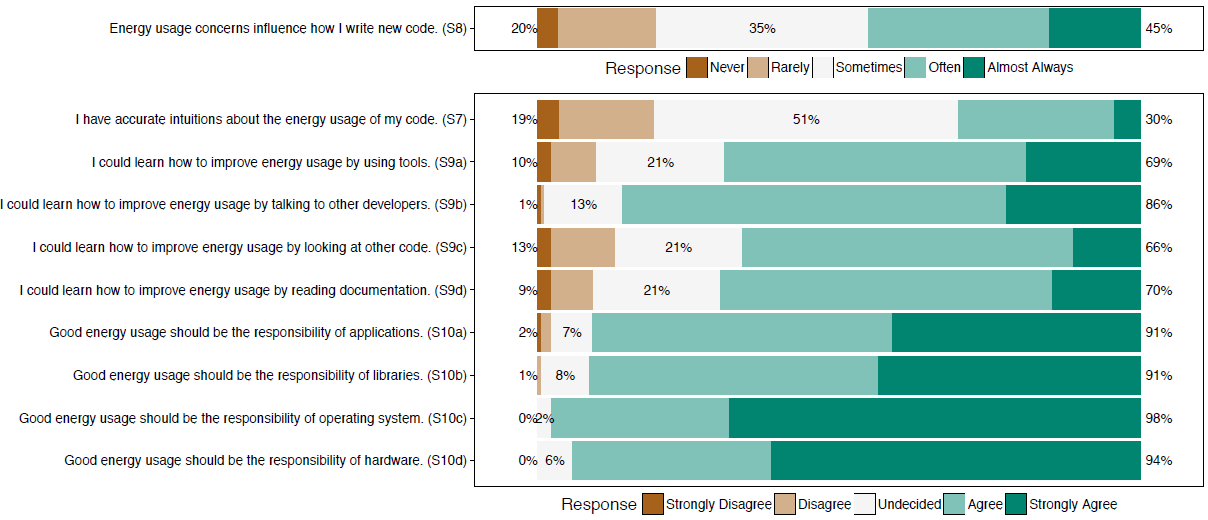
\includegraphics[width=1\textwidth]{MemoireMaster-NestorSkoczylas/figures/Déclarations et réponses des praticiens expérimentés liées à la construction.png}
    \caption{Déclarations et réponses des praticiens expérimentés liées à la construction}
    \label{fig:declaration-reponses-praticien}
\end{figure}

Certains utilisateurs, comme le souligne l'étude~\cite{EmpiricalStudy}, estiment que \emph{« Good energy usage should be the responsibility of applications »}. Cependant, il est crucial de reconnaître que cette responsabilité est partagée, comme le montre la figure \ref{fig:declaration-reponses-praticien}. Cette figure montre que les praticiens expérimentés reconnaissent la responsabilité partagée dans l'utilisation durable des logiciels, tout en soulignant l'importance de la documentation et des outils pour les aider à améliorer leur consommation d'énergie.


Comme le souligne l'étude~\cite{SafetySecuritySustainability}, \emph{« Software engineers can contribute to sustainability by designing software systems that minimize indirect impacts and by educating users about the impacts of their actions. »} . Cela implique :

\begin{itemize}
    \item \textbf{Une conception logicielle efficace :} Choisir des technologies économes en énergie, optimiser les performances du code et minimiser la consommation de ressources.
    \item \textbf{L'optimisation des logiciels :} Mettre à jour régulièrement les logiciels pour bénéficier des dernières optimisations et corriger les bugs qui peuvent affecter la consommation d'énergie.
    \item \textbf{La formation des utilisateurs :} Sensibiliser les utilisateurs aux enjeux de la durabilité logicielle et leur fournir les outils nécessaires pour adopter des pratiques durables.
\end{itemize}


En adoptant des pratiques éclairées et en comprenant l'impact de leurs actions, les utilisateurs peuvent également jouer un rôle crucial dans la durabilité logicielle. Cela implique :

\begin{itemize}
    \item \textbf{Une utilisation responsable des logiciels :} Réduire l'utilisation inutile des logiciels, fermer les programmes lorsqu'ils ne sont pas utilisés et privilégier les solutions logicielles économes en énergie.
    \item \textbf{Comprendre l'impact de ses actions :} Savoir comment les choix de logiciels et les actions quotidiennes peuvent affecter la consommation d'énergie et l'empreinte environnementale.
    \item \textbf{Tirer parti des ressources pédagogiques :} Exploiter la documentation, les tutoriels et les guides mis à disposition par les développeurs pour apprendre à utiliser les logiciels de manière durable.
\end{itemize}


L'intégration de la durabilité environnementale en tant qu'exigence non fonctionnelle est essentielle pour une mise en œuvre réussie. Cette notion est soulignée dans~\cite{SafetySecuritySustainability}, qui stipule que : \emph{« To support the transition to sustainability, environmental sustainability must be explicitly considered as a nonfunctional requirement in the software engineering process. »} Il est crucial de formaliser les considérations de durabilité dans le cycle de vie du développement logiciel. Cela implique de les intégrer dès les phases initiales de conception et de les maintenir tout au long du processus de développement, y compris la phase de test et de déploiement.


L'étude publiée dans~\cite{ImpactGreenFeedback} identifie une lacune cruciale : \emph{« Green feedback helps in raising awareness, but users lack the knowledge and tools to apply software behavioral changes. »} Il ne suffit pas de fournir aux utilisateurs des commentaires sur l'impact environnemental de leurs choix. Pour combler le fossé entre la sensibilisation et l'action, les développeurs et autres parties prenantes doivent s'engager à :

\begin{itemize}
    \item Développer des outils conviviaux qui permettent aux utilisateurs de suivre leur utilisation de logiciels, de comprendre son impact environnemental et de faire des choix éclairés.
    \item Organiser des campagnes continues d'éducation et de sensibilisation qui dotent les utilisateurs des connaissances et des compétences nécessaires pour contribuer à une utilisation durable des logiciels.
\end{itemize}


La communauté du développement de logiciels a un rôle crucial à jouer dans la construction d'un avenir numérique durable. En adoptant une approche collaborative et proactive, nous pouvons transformer l'ingénierie logicielle verte en une force positive pour l'environnement.

% Responsabilité partagée et sensibilisation des utilisateurs
%~\cite{EmpiricalStudy} "Energy usage should be a shared responsibility."
%~\cite{EmpiricalStudy} "I could learn how to improve energy usage by reading documentation."
%~\cite{EmpiricalStudy} "Good energy usage should be the responsibility of applications."
%~\cite{SafetySecuritySustainability} "To support the transition to sustainability, environmental sustainability must be explicitly considered as a nonfunctional requirement in the software engineering process."
%~\cite{SafetySecuritySustainability} "Software engineers can contribute to sustainability by designing software systems that minimize indirect impacts and by educating users about the impacts of their actions."
%~\cite{ImpactGreenFeedback} "Green feedback helps in raising awareness, but users lack the knowledge and tools to apply software behavioral changes."

\subsection{Formation des utilisateurs et retour d'information}
L'éducation et l'implication des utilisateurs sont des piliers fondamentaux pour une utilisation responsable et durable des logiciels. En effet, leur compréhension des enjeux environnementaux et de leur rôle crucial dans l'adoption de pratiques durables est essentielle.


L'écoute des besoins et des attentes des utilisateurs est tout aussi importante. Comme le souligne l'étude~\cite{EmpiricalStudy}, les utilisateurs expriment un réel désir d'apprendre et de s'améliorer : \emph{« I could learn how to improve energy usage by reading documentation. »} La figure \ref{fig:declaration-reponses-praticien} montre que 70\% des praticiens expérimentés estiment que la documentation peut les aider à améliorer leur consommation d'énergie. Cela confirme le besoin crucial de ressources éducatives accessibles et attractives pour répondre à la demande des utilisateurs.Répondre à cette demande par des ressources éducatives accessibles et attractives est donc un enjeu majeur. Cela passe par la création de :

\begin{itemize}
    \item Documentations claires et concises qui exposent l'impact environnemental des logiciels et proposent des solutions concrètes pour l'optimiser.
    \item Tutoriels interactifs et campagnes de sensibilisation qui engagent les utilisateurs et transmettent de manière ludique l'importance de pratiques durables.
\end{itemize}

En outre, responsabiliser les utilisateurs en leur offrant les connaissances et les outils nécessaires est crucial. Comme le souligne~\cite{SafetySecuritySustainability}, \emph{« Software engineers can contribute to sustainability by [...] educating users about the impacts of their actions. »} En dotant les utilisateurs de moyens d'action concrets, nous leur permettons de participer activement à la construction d'un écosystème logiciel durable.


L'étude de~\cite{ImpactGreenFeedback} souligne l'importance de \emph{« Green feedback helps in raising awareness »}. Cependant, elle met également en lumière ses limites :
\begin{itemize}
    \item \textbf{Manque de connaissances et d'outils :} \emph{« Users lack the knowledge and tools to apply software behavioral changes. »} Fournir des commentaires ne suffit pas nécessairement à engendrer des changements significatifs.
    \item \textbf{Intrusion et surcharge d'informations :} \emph{« Green feedback tools must be minimal and seamlessly integrated to avoid being distracted. »} Les mécanismes de feedback doivent être centrés sur l'utilisateur, non intrusifs et fournir des informations exploitables pour responsabiliser les utilisateurs sans les submerger.
\end{itemize}


Pour dépasser ces limites, il est essentiel de repenser la rétroaction verte. Voici quelques pistes d'amélioration :
\begin{itemize}
    \item Développez des outils conviviaux qui suivent l’utilisation des logiciels, visualisent leur impact environnemental et proposent des suggestions d’optimisation.
    \item Intégrez des mécanismes de feedback de manière transparente dans l'interface du logiciel pour minimiser les distractions et encourager l'engagement des utilisateurs.
    \item Fournissez des informations claires et exploitables grâce à des commentaires pour aider les utilisateurs à comprendre l'impact de leurs choix et à prendre des décisions éclairées concernant leur utilisation du logiciel.
\end{itemize}


L'éducation et la rétroaction efficace des utilisateurs constituent les piliers d'un avenir numérique durable. En comblant le déficit de connaissances et en responsabilisant les utilisateurs, nous pouvons construire un écosystème logiciel plus collaboratif et respectueux de l'environnement.


L'éducation permet aux utilisateurs de comprendre l'impact environnemental de leurs choix. Des ressources éducatives accessibles et attractives, telles que des tutoriels interactifs et des campagnes de sensibilisation, peuvent les aider à adopter des pratiques logicielles durables.


La rétroaction efficace fournit aux utilisateurs des informations exploitables sur leur consommation d'énergie. Des outils conviviaux qui suivent l'utilisation des logiciels, visualisent l'impact environnemental et proposent des suggestions d'optimisation peuvent les inciter à agir de manière responsable.


En combinant ces deux approches, nous pouvons créer un cercle vertueux. Les utilisateurs informés et responsabilisés peuvent influencer les développeurs, les incitant à concevoir des logiciels plus économes en énergie et à intégrer la durabilité comme une exigence fondamentale.

% Formation des utilisateurs et retour d'information
%~\cite{EmpiricalStudy} "I could learn how to improve energy usage by reading documentation."
%~\cite{SafetySecuritySustainability} "Software engineers can contribute to sustainability by designing software systems that minimize indirect impacts and by educating users about the impacts of their actions."
%~\cite{ImpactGreenFeedback} "Green feedback helps in raising awareness, but users lack the knowledge and tools to apply software behavioral changes."
%~\cite{ImpactGreenFeedback} "Green feedback tools must be minimal and seamlessly integrated to avoid being distracted."

\subsection{Concevoir pour un comportement durable}
La conception de logiciels durables ne se limite pas à l'optimisation technique. Elle vise également à influencer le comportement des utilisateurs vers des pratiques plus responsables et respectueuses de l'environnement.


L'étude de~\cite{SafetySecuritySustainability} met en lumière une perspective intéressante : \emph{« If sustainability policies and standards are put in place and software engineers prioritize them in the systems they develop, future technology may significantly contribute indirectly to influencing the behavior of users who interact with those systems in some ways while directly contributing to saving the planet. »} Ce passage souligne le pouvoir des logiciels bien conçus d'inciter les utilisateurs à adopter des comportements plus durables. En intégrant des fonctionnalités et des caractéristiques orientées vers la durabilité, les logiciels peuvent aller au-delà de leur simple fonction et devenir de véritables catalyseurs de changement.


Comment les logiciels peuvent-ils influencer les utilisateurs ?


Plusieurs leviers de conception peuvent être utilisés pour encourager les pratiques éco-responsables :

\begin{itemize}
    \item \textbf{Transparence et feedback écologique :} Informer les utilisateurs sur l'impact environnemental de leurs actions et de l'utilisation du logiciel les sensibilise et les incite à faire des choix plus informés.
    \item \textbf{Nudges et architecture de choix :} Des suggestions subtiles et une organisation réfléchie de l'interface peuvent guider les utilisateurs vers des options plus éco-responsables, sans pour autant limiter leur liberté de choix.
    \item \textbf{Gamification et motivation :} L'intégration d'éléments ludiques, comme des points et des classements, peut rendre l'utilisation durable du logiciel plus attrayante et motivante.
    \item \textbf{Par défaut durable :} Définir des options par défaut éco-responsables peut inciter les utilisateurs à adopter ces pratiques sans effort supplémentaire.
\end{itemize}


L'article~\cite{SafetySecuritySustainability} met en exergue l'importance cruciale de formaliser la prise en compte de la durabilité dans le développement logiciel. Il affirme : \emph{« To support the transition to sustainability, environmental sustainability must be explicitly considered as a nonfunctional requirement in the software engineering process. »} En d'autres termes, la durabilité ne doit pas être reléguée au second plan, mais bel et bien s'ériger comme une exigence fondamentale au même titre que la sécurité, la performance ou la maintenabilité.


L'article~\cite{SafetySecuritySustainability} rappelle le rôle crucial des ingénieurs logiciels dans la promotion de la durabilité : \emph{« Software engineers can contribute to sustainability by designing software systems that minimize indirect impacts and by educating users about the impacts of their actions. »} Leur influence sur le comportement des utilisateurs se manifeste à travers plusieurs leviers :
\begin{itemize}
    \item \textbf{Conception de fonctionnalités durables :} Intégrer des options favorisant l'efficacité des ressources et décourageant le gaspillage permet d'agir directement sur l'impact environnemental du logiciel.
    \item \textbf{Feedback écologique transparent :} Fournir des informations claires et accessibles au sein du logiciel sensibilise les utilisateurs aux implications de leurs choix et encourage des pratiques plus responsables.
    \item \textbf{Optimisation énergétique intrinsèque :} Comme le souligne~\cite{GreenMeasurementStructure}, \emph{« The software can minimise power consumption by being more energy-efficient (i.e., by becoming greener); utilizing lesser power or adopting more sustainable and supported procedures will diminish the environmental effects of software used by governments, organizations, and people. »} L’importance de concevoir des logiciels intrinsèquement économes en énergie, réduisent dès le départ leur empreinte environnementale.
\end{itemize}


La communauté des développeurs de logiciels possède un pouvoir unique : créer des logiciels qui minimisent leur propre impact environnemental tout en influençant positivement le comportement des utilisateurs. Cette double approche est essentielle pour construire un avenir numérique plus durable.


Concevoir des logiciels durables ne se résume pas à une simple optimisation technique. Il s'agit d'une démarche holistique qui prend en compte l'ensemble du cycle de vie du logiciel et intègre la durabilité comme une exigence fondamentale.

% Concevoir pour un comportement durable
%~\cite{SafetySecuritySustainability} "If sustainability policies and standards are put in place and software engineers prioritize them in the systems they develop, future technology may significantly contribute indirectly to influencing the behavior of users who interact with those systems in some ways while directly contributing to saving the planet."
%~\cite{SafetySecuritySustainability} "To support the transition to sustainability, environmental sustainability must be explicitly considered as a nonfunctional requirement in the software engineering process."
%~\cite{SafetySecuritySustainability} "Software engineers can contribute to sustainability by designing software systems that minimize indirect impacts and by educating users about the impacts of their actions."
%~\cite{GreenMeasurementStructure} "The software can minimise power consumption by being more energy-efficient (i.e., by becoming greener); utilizing lesser power or adopting more sustainable and supported procedures will diminish the environmental effects of software used by governments, organizations, and people."

\paragraph{}
Le développement durable des logiciels ne se limite pas aux efforts des développeurs. Les utilisateurs jouent un rôle crucial en adoptant des pratiques responsables et en contribuant à l'utilisation efficace et écologique des logiciels. 
Cette section explore les moyens de promouvoir un comportement durable chez les utilisateurs, en s'attaquant aux aspects clés de la sensibilisation, de la formation et de la conception logicielle.


Sensibilisation et responsabilisation des utilisateurs :
\begin{itemize}
    \item Responsabilité partagée : La durabilité logicielle est un effort collectif. Développeurs, utilisateurs et parties prenantes doivent collaborer pour minimiser l'impact environnemental des logiciels.
    \item Sensibilisation et éducation : Fournir aux utilisateurs des ressources accessibles et compréhensibles pour les sensibiliser aux implications énergétiques de leurs actions et les inciter à adopter des pratiques durables.
    \item Outils et information : Développer des outils conviviaux qui permettent aux utilisateurs de suivre leur utilisation des logiciels et de comprendre son impact environnemental.
    \item Campagnes de sensibilisation : Organiser des campagnes continues pour diffuser des informations sur l'importance des pratiques logicielles durables et responsabiliser les utilisateurs.
\end{itemize}


Formation et responsabilisation des utilisateurs :
\begin{itemize}
    \item Combler le déficit de connaissances : Fournir aux utilisateurs des ressources éducatives facilement accessibles, telles que des tutoriels, des guides et des formations, pour leur donner les compétences nécessaires pour contribuer à la durabilité logicielle.
    \item Feedback efficace : Concevoir des mécanismes de feedback non intrusifs et exploitables qui intègrent des suggestions d'optimisation et des informations claires sur l'impact environnemental des choix des utilisateurs.
    \item Autonomisation des utilisateurs : Donner aux utilisateurs les moyens de prendre des décisions éclairées en matière d'utilisation des logiciels en leur fournissant des informations et des outils pertinents.
\end{itemize}


Concevoir pour un comportement durable :
\begin{itemize}
    \item Intentionnalité et influence : Concevoir des logiciels qui incitent les utilisateurs à adopter des pratiques plus responsables et respectueuses de l'environnement.
    \item Fonctionnalités durables : Intégrer des fonctionnalités qui favorisent l'efficacité des ressources et découragent le gaspillage.
    \item Information accessible : Fournir des informations claires et contextuelles au sein du logiciel sur l'impact environnemental des actions des utilisateurs.
    \item Optimisation de l'efficacité : Concevoir des logiciels intrinsèquement économes en énergie pour réduire leur empreinte environnementale dès le départ.
\end{itemize}


En sensibilisant, en formant et en responsabilisant les utilisateurs, et en concevant des logiciels qui encouragent des pratiques durables, la communauté des développeurs de logiciels peut créer un avenir plus vert et plus durable. La collaboration et l'engagement de tous les acteurs sont essentiels pour réaliser cet objectif.

%%%%%%%%%%%%%%%%%%%%%%%%%%%%%%%%%%%%

\paragraph{Conclusion}
Ce chapitre a exploré l'influence cruciale des pratiques individuelles des développeurs sur la durabilité des logiciels. Au-delà des aspects techniques, il a mis en lumière l'importance de la responsabilité individuelle et de l'engagement dans la création d'un avenir numérique plus vert.


Que faut-il retenir de ce chapitre ?
\begin{enumerate}
    \item Sensibilisation et connaissances : La sensibilisation aux impacts environnementaux du développement logiciel est le point de départ. Les développeurs doivent acquérir les connaissances nécessaires pour prendre des décisions éclairées et adopter des pratiques durables.
    \item Engagement et responsabilité : Chaque développeur est responsable de l'empreinte environnementale de son code. Adopter une attitude pro-active et responsable est crucial pour contribuer à un avenir plus durable.
    \item Pratiques et outils durables : De nombreuses pratiques et outils existent pour aider les développeurs à réduire l'impact environnemental de leur travail. Il est important de les connaître et de les utiliser de manière optimale.
    \item Collaboration et partage des connaissances : La collaboration entre les développeurs, les équipes et les organisations est essentielle pour faire progresser les pratiques durables dans l'industrie du logiciel.
    \item Mesure et évaluation : Suivre et évaluer l'impact environnemental des logiciels est crucial pour identifier les domaines d'amélioration et mesurer les progrès accomplis.
    \item Engagement continu : La durabilité logicielle n'est pas une destination finale, mais un voyage continu. Il est important de rester engagé et de s'adapter aux nouvelles technologies et aux meilleures pratiques émergentes.
\end{enumerate}


En résumé, les développeurs ont le pouvoir de jouer un rôle crucial dans la création d'un avenir numérique plus durable. 
En adoptant une conscience accrue, en s'engageant à des pratiques responsables et en collaborant avec la communauté, ils peuvent contribuer à un changement positif et significatif.

\paragraph{Transition vers Intégration de la Durabilité à Différentes Échelles dans le Développement Logiciel}
Le deuxième chapitre a mis en lumière l'importance des pratiques individuelles des développeurs dans la construction de logiciels durables. Nous avons conclu en soulignant la nécessité d'une responsabilité individuelle et d'un engagement continu pour un avenir numérique plus écologique.


Or, la durabilité logicielle ne se limite pas aux actions individuelles. Elle exige une approche globale qui intègre des pratiques durables à différentes échelles, allant des projets et des équipes de développement jusqu'à la stratégie d'entreprise. C'est précisément l'objet du \ref{pratique-globale}, qui explore comment intégrer la durabilité à différentes échelles dans le développement logiciel.


Ce chapitre examinera comment les projets logiciels peuvent être planifiés et exécutés en tenant compte de la durabilité. Il se penchera également sur les pratiques durables au niveau des équipes de développement et sur la manière dont les entreprises peuvent aligner leur stratégie sur les objectifs de durabilité logicielle.


En explorant ces différentes échelles d'action, le \ref{pratique-globale} vise à démontrer l'importance d'une approche multidimensionnelle pour un développement logiciel véritablement durable.

% Chapter 3

\chapter{Intégration de la Durabilité à Différentes Échelles dans le Développement Logiciel}	%The main chapter title
\label{pratique-globale}

%%%%%%%%%%%%%%%%%%%%%%%%%%%%%%%%%%%%

La durabilité dans le génie logiciel ne se limite pas aux pratiques individuelles et aux équipes de développement. Ce chapitre explore l'intégration de la durabilité à l'échelle des projets logiciels, des équipes et de la stratégie d'entreprise.


Le chapitre se compose de trois sections distinctes, chacune offrant un aperçu des pratiques durables à grande échelle qui façonnent l'avenir du génie logiciel durable. La première section examine les méthodes et les outils pour mettre en œuvre des pratiques durables au niveau des projets logiciels (Section~\ref{sec:pratiques-projets}). La deuxième section explore les initiatives et les actions concrètes pour encourager la durabilité au sein des équipes de développement (Section~\ref{sec:pratiques-equipe}). La dernière section analyse l'alignement de la stratégie de \acrshort{rse} avec les objectifs de durabilité dans le développement logiciel (Section~\ref{sec:rse-durabilite}).

%%%%%%%%%%%%%%%%%%%%%%%%%%%%%%%%%%%%

\section{Stratégies pour Intégrer la Durabilité dans les Projets Logiciels}
\label{sec:pratiques-projets}

%%%%%%%%%%%%%%%%%%%%%%%%%%%%%%%%%%%%
La durabilité ne peut être atteinte qu'à travers des projets logiciels bien planifiés et exécutés.

\subsection{Gestion de projet et outils}
Une gestion de projet efficace et l'adoption d'outils appropriés sont indispensables à la mise en œuvre réussie de pratiques d'ingénierie logicielle écologiques. 


L'étude publiée dans l'article "Green Software Engineering with Agile Methods"~\cite{GreenAgileMethods} fait valoir l'intérêt de tirer parti des méthodologies de gestion de projet existantes : \emph{« In order to implement the presented procedure models, the actors in software development projects need to be supported by tools: Besides educational material regarding sustainability issues, specialized software, and spread sheets, these are tools, well-known in the field of software development (e.g. Continuous Integration). »} Ce constat suggère que des pratiques établies telles que l'intégration continue (IC) peuvent être étendues pour intégrer des considérations relatives à la durabilité.


La même étude dans~\cite{GreenAgileMethods} précise le potentiel de l'intégration continue pour le développement de logiciels écologiques : \emph{« Using Continuous Integration enables developer teams to minimize their integration effort and their feedback on current software quality. We wanted to use these assets on rating the energy efficiency of software. This is why we developed a model to integrate performance and energy measurement into Continuous Integration. »} En intégrant la mesure de la performance et de l'énergie dans le processus d'intégration continue, les développeurs peuvent recevoir un retour d'information continu sur l'impact environnemental de leur code, ce qui leur permet d'identifier et de corriger les inefficacités tout au long du cycle de développement.


La recherche présentée dans "The GREENSOFT Model"~\cite{GreenSoftModel} explore les modèles dédiés au développement de logiciels écologiques. L'étude mentionne le \emph{« Grand Management Information Design »} comme une solution potentielle pour aborder les questions de durabilité lors de la conception et du développement de logiciels. Un examen plus approfondi de ces modèles et de leur application pratique peut fournir des informations précieuses à la communauté des développeurs de logiciels.


Si les méthodologies et les outils de gestion de projet existants offrent une base solide, le besoin d'outils spécialisés dans le développement de logiciels écologiques est également évident. Comme indiqué dans cette même étude~\cite{GreenSoftModel}, ces outils peuvent comprendre :
\begin{itemize}
    \item Du matériel pédagogique pour sensibiliser les développeurs et leur donner les connaissances nécessaires.
    \item Des logiciels spécialisés pour mesurer, analyser et optimiser l'efficacité énergétique des logiciels.
    \item Des tableurs et autres outils de gestion des données pour suivre les progrès et prendre des décisions fondées sur des données.
\end{itemize}


Les chefs de projet et les équipes de développement peuvent être bien équipés pour naviguer dans les complexités de l'ingénierie logicielle écologique et atteindre leurs objectifs de durabilité, grâce à des pratiques de gestion de projet bien établies, à l'intégration de considérations écologiques dans des outils existants tels que l'IC, et à l'exploration et l'adoption d'outils spécialisés dans le développement de logiciels écologiques.

% Gestion de projet et outils
%~\cite{GreenAgileMethods} "In order to implement the presented procedure models, the actors in software development projects need to be supported by tools: Besides educational material regarding sustainability issues, specialized software, and spread sheets, these are tools, well-known in the field of software development (e.g. Continuous Integration)."
%~\cite{GreenAgileMethods} "Using Continuous Integration enables developer teams to minimize their integration effort and their feedback on current software quality. We wanted to use these assets on rating the energy efficiency of software. This is why we developed a model to integrate performance and energy measurement into Continuous Integration."
%~\cite{GreenSoftModel} "Arndt et al. discuss implications of evolving releases of a widely used text processor and relate these to Green IT and SD. As a solution to cope with sustainability issues during software design and development, they propose the so called “Grand Management Information Design”."

\subsection{Mesure et évaluation de la durabilité}
L'étude d'Albertao et al. dans~\cite{GreenSoftModel} propose de tirer parti des propriétés et des mesures de qualité logicielle établies : \emph{« Albertao et al. interpret common software quality properties and associated metrics on the background of SD. They classify the quality properties into development, usage, and process related properties. »} Les cadres de qualité existants peuvent donc servir de base à l'évaluation de la durabilité des logiciels.


Le modèle GREENSOFT se concentre sur les \emph{« Sustainability Criteria and Metrics »}. 
Ce modèle :
\begin{enumerate}
    \item \emph{« classification of criteria and metrics for evaluating a software product’s sustainability »}~\cite{GreenSoftModel}
    \item \emph{« Three categories of sustainability criteria and metrics for software products: Common Quality Criteria and Metrics, Directly Related Criteria and Metrics, and Indirectly Related Criteria and Metrics. »}~\cite{GreenSoftModel}
\end{enumerate}
Cette catégorisation permet de faire la différence entre les mesures de qualité établies et celles qui sont spécifiquement conçues pour évaluer l'impact environnemental d'un produit logiciel.


Selon~\cite{SafetySecuritySustainability}, une vision holistique de la durabilité est cruciale : \emph{« Sustainability in software engineering not only encompasses energy efficiency and green IT, but must also consider the second- and third-order impacts of software systems. »} 
Cette remarque démontre la volonté de prendre en compte l'impact environnemental plus large des logiciels, au-delà de la seule consommation d'énergie.


Cette étude propose d'adapter l'\acrfull{acv} à l'ingénierie logicielle : \emph{« For assessment techniques to address quality assurance, we propose evaluating and adapting LCA to software engineering and making use of environmental impact assessment in software engineering. »} 
L'\acrshort{acv} est une technique utilisée pour évaluer l'impact environnemental d'un produit tout au long de son cycle de vie. 
L'adaptation de cette approche au développement de logiciels peut fournir des informations précieuses sur l'empreinte environnementale des produits logiciels.


Le modèle présenté dans~\cite{IntegrationSustainabilityMetrics} témoigne de l'importance de l'intégration des mesures de durabilité dans la réalisation des projets : \emph{« The proposed model enables the measurement of the sustainability of code, thereby fostering a more comprehensive understanding of the relationship between project delivery performance and sustainable practices. »} 
Cette intégration a permis aux développeurs et aux chefs de projet d'évaluer l'impact de leurs efforts en matière de développement durable sur les résultats du projet.


En s'appuyant sur les cadres de qualité existants, en utilisant le modèle GREENSOFT, en tenant compte des impacts plus larges sur la durabilité, en adaptant éventuellement les techniques d'\acrshort{acv} et en intégrant des mesures de durabilité dans la réalisation des projets, la communauté des développeurs de logiciels peut établir un cadre solide pour mesurer et évaluer l'impact des produits logiciels sur l'environnement.

% Mesure et évaluation de la durabilité
%~\cite{GreenSoftModel} "Albertao et al. interpret common software quality properties and associated metrics on the background of SD. They classify the quality properties into development, usage, and process related properties."
%~\cite{GreenSoftModel} "The second part of the GREENSOFT Model is called Sustainability Criteria and Metrics. It covers common metrics and criteria for the measurement of software quality and it allows a classification of criteria and metrics for evaluating a software product’s sustainability."
%~\cite{GreenSoftModel} "Our model has the ability to represent three categories of sustainability criteria and metrics for software products: Common Quality Criteria and Metrics, Directly Related Criteria and Metrics, and Indirectly Related Criteria and Metrics."
%~\cite{SafetySecuritySustainability} "Sustainability in software engineering not only encompasses energy efficiency and green IT, but must also consider the second- and third-order impacts of software systems."
%~\cite{SafetySecuritySustainability} "For assessment techniques to address quality assurance, we propose evaluating and adapting LCA to software engineering and making use of environmental impact assessment in software engineering."
%~\cite{IntegrationSustainabilityMetrics} "The proposed model enables the measurement of the sustainability of code, thereby fostering a more comprehensive understanding of the relationship between project delivery performance and sustainable practices."

\subsection{Cadres et modèles de durabilité}
En se basant sur l'accent mis par le modèle GREENSOFT~\cite{GreenSoftModel} sur les critères et les mesures de durabilité (évoqués précédemment), il reconnaît la possibilité de trouver des solutions plus larges : \emph{« Besides reflecting the proposed life cycle of a software product, there are further methods that support software architects, designers, and developers in producing green and sustainable software applications. »} D'où l'existence de cadres supplémentaires qui complètent le modèle GREENSOFT.


La théorie de la durabilité stratifiée, présentée dans [SustainableStratifiedTheory], offre une perspective nuancée :
\begin{itemize}
    \item La durabilité à multiples facettes : Elle met l'accent sur la \emph{« stratified and multisystemic nature of sustainability. »}~\cite{SustainableStratifiedTheory} La durabilité englobe divers aspects au-delà de l'impact sur l'environnement;
    \item Processus et produit : Le modèle fait la distinction entre le processus de développement du logiciel et le produit logiciel qui en résulte. Les considérations de durabilité s'appliquent aux deux.
\end{itemize}


La théorie met en évidence quatre dimensions clés de la durabilité :
\begin{enumerate}
    \item L'environnement : Minimiser l'empreinte environnementale du produit logiciel;
    \item Sociale : Prise en compte de l'impact social du logiciel sur les utilisateurs et les parties prenantes;
    \item Économique : Garantir la viabilité économique du logiciel et l'allocation responsable des ressources;
    \item Technique : Maintenir la qualité technique et les performances du logiciel tout en optimisant la durabilité.
\end{enumerate}
Il est essentiel de prendre en compte toutes ces dimensions pour parvenir à une véritable durabilité des logiciels.


La recherche dans~\cite{SustainabilityAwarenessFramework} et~\cite{SustainabilityRequirementsEngineering} explore l'intégration de la durabilité dans les méthodologies de développement existantes :
\begin{itemize}
    \item Sustainability-Aware Scrum Framework : Ce cadre vise à fournir des lignes directrices pour l'intégration des considérations de durabilité dans la méthodologie Agile Scrum.
    \item \acrfull{susaf} : il propose un ensemble de questions et d'instructions pour guider les ingénieurs en exigences dans leurs discussions sur la durabilité avec les parties prenantes.
    \item Processus itératif avec listes de contrôle : Cette approche utilise des listes de contrôle pour identifier les besoins en matière de durabilité dans différentes dimensions au cours de la phase d'ingénierie des exigences.
\end{itemize}
Ces cadres démontrent les efforts en cours pour faire de la durabilité une partie inhérente du processus de développement de logiciels.


La communauté des développeurs de logiciels peut établir une approche globale de la conception, du développement et du déploiement de solutions logicielles durables en s'appuyant sur des cadres tels que le modèle GREENSOFT, la théorie de la durabilité stratifiée et des adaptations des méthodologies existantes tenant compte de la durabilité.

% Cadres et modèles de durabilité
%~\cite{GreenSoftModel} "Arndt et al. discuss implications of evolving releases of a widely used text processor and relate these to Green IT and SD. As a solution to cope with sustainability issues during software design and development, they propose the so called “Grand Management Information Design”."
%~\cite{GreenSoftModel} "Besides reflecting the proposed life cycle of a software product, there are further methods that support software architects, designers, and developers in producing green and sustainable software applications."
%~\cite{SustainableStratifiedTheory} "The goal of this model is to explain how sustainability relates to software development based on existing qualitative research and to provide a more nuanced view of the stratified and multisystemic nature of sustainability according to our observations from the meta-synthesis."
%~\cite{SustainableStratifiedTheory} "The model separates the software process from the software product to illustrate that sustainability is a property of both and while the nature of the software development process affects the resulting software system, a sustainable process does not guarantee a sustainable product or vice versa."
%~\cite{SustainableStratifiedTheory} "The model depicts four dimensions or pillars of sustainability—environmental, social, economic and technical. All four dimensions apply to software products."
%~\cite{SustainabilityAwarenessFramework} "Our future work will support the development of a Sustainability-Aware Scrum Framework, which could provide guidelines on how to consider sustainability issues in ASD, based on the original Scrum framework."
%~\cite{SustainabilityRequirementsEngineering} "Duboc et al. present a sustainability awareness framework (SuSAF) that includes a set of instructions and questions that can be used by requirements engineers to guide discussions on sustainability with the stakeholders."
%~\cite{SustainabilityRequirementsEngineering} "Paech, Moreira, Araujo, and Kaiser introduce an iterative process with two checklists. The first checklist can be used to identify needs of each sustainability dimension for a system, e.g. little pollution and little waste in the environmental dimension or high customer satisfaction and little cost in the economical dimension."
%~\cite{SustainabilityRequirementsEngineering} "Penzenstadler et al. describe the application of the framework in an educational context."

\subsection{Comportement et pratiques des développeurs}
Le succès de l'ingénierie logicielle écologique dépend non seulement des solutions techniques, mais aussi des attitudes et des pratiques des développeurs de logiciels.


Conformément à l'article~\cite{SustainableEngNeglectedPerspective}, il est utile de disposer de \emph{« empirically validated practices and guidelines for processes, policies, practices to ensure engineer’s sustainability. »} En effet, il est de plus en plus difficile d'établir des directives pratiques permettant aux développeurs d'intégrer les considérations relatives à la durabilité dans leur travail quotidien. Ces lignes directrices peuvent porter sur divers aspects du cycle de développement des logiciels, de la conception et du codage au déploiement et à la maintenance.


La recherche dans~\cite{SustainableEngNeglectedPerspective} évoque une \emph{« taxonomy of factors and guidelines »} qui peut influencer la prise de décision des développeurs : \emph{« The resulting taxonomy [...] will influence the decision-making models and methods to take into consideration the concepts of sustainability. »} Cette taxonomie peut fournir un cadre permettant aux développeurs d'évaluer leurs choix et de prendre des décisions éclairées qui donnent la priorité à la durabilité tout au long du processus de développement.


La même étude fait état de la difficulté de comprendre les interrelations entre les différents facteurs qui influencent le comportement des promoteurs : \emph{« The factors would also serve as a foundation for future research to find interrelations between them, categorize them and devise ways to control them. »} Ces facteurs peuvent inclure les éléments suivants :
\begin{itemize}
    \item Connaissance et sensibilisation aux principes de l'ingénierie logicielle écologique.
    \item Accès aux outils et aux ressources qui soutiennent le développement durable.
    \item Culture organisationnelle et engagement des dirigeants en faveur du développement durable.
\end{itemize}
La recherche de ces facteurs et de leurs interactions permettra à la communauté des développeurs de logiciels de concevoir des interventions et des stratégies efficaces pour promouvoir les pratiques de développement durable parmi les développeurs.


La promotion d'une culture du développement durable au sein de la communauté des développeurs de logiciels nécessite une approche sur plusieurs fronts.  L'élaboration de lignes directrices pratiques, la mise en place d'un cadre décisionnel pour la durabilité et la compréhension des facteurs influençant le comportement des développeurs sont autant d'étapes cruciales.

% Comportement et pratiques des développeurs
%~\cite{SustainableEngNeglectedPerspective} "The third outcome is the development of empirically validated practices and guidelines for processes, policies, practices to ensure engineer’s sustainability." 
%~\cite{SustainableEngNeglectedPerspective} "The resulting taxonomy of factors and guidelines will influence the decision-making models and methods to take into consideration the concepts of sustainability." 
%~\cite{SustainableEngNeglectedPerspective} "The factors would also serve as a foundation for future research to find interrelations between them, categorize them and devise ways to control them."

\subsection{Collaboration et sensibilisation}
La collaboration entre les parties prenantes et la sensibilisation aux pratiques d'ingénierie logicielle écologique sont fondamentales pour une mise en œuvre réussie.


La publication~\cite{SustainabilityAwarenessFramework} illustre l'application pratique de cadres tels que \acrshort{susaf} : \emph{« In this experience paper, we present the results of two case studies from ongoing agile development projects where the Sustainability Awareness Framework was applied. »} Ce document témoigne de la valeur de l'utilisation de ces cadres pour faciliter les discussions collaboratives et intégrer les considérations de durabilité dans les processus de développement agile. L'étude poursuit en mentionnant des \emph{« sustainability workshops based on SusAF »} et la \emph{« mapping identified sustainability effects to the product backlog items »} comme exemples concrets de l'application du cadre.


Bien que les cadres tels que \acrshort{susaf} n'aient pas été conçus à l'origine pour les méthodologies agiles,~\cite{SustainabilityRequirementsEngineering} reconnaît leur applicabilité potentielle : \emph{« It is remarkable that none of these approaches directly target the application within an agile software development setting, although this does not mean that they are not applicable in such a setting. »} On peut donc en déduire que les cadres existants peuvent être adaptés et intégrés dans des flux de travail agiles afin de répondre aux préoccupations en matière de durabilité.


Une autre approche décrite dans~\cite{SustainabilityRequirementsEngineering} consiste à utiliser des listes de contrôle pour \emph{« to identify needs of each sustainability dimension for a system. »} Cette approche structurée peut être utilisée en collaboration pendant la phase d'ingénierie des exigences afin de s'assurer que tous les aspects de la durabilité sont pris en compte. La nature itérative du processus permet de l'affiner continuellement au fur et à mesure de l'avancement du projet.


L'application des cadres dans des contextes éducatifs, comme mentionné dans~\cite{SustainabilityRequirementsEngineering}, joue un rôle crucial dans la sensibilisation et la construction d'une future génération de développeurs dotés d'une expertise en ingénierie logicielle écologique : \emph{« Penzenstadler et al. describe the application of the framework in an educational context. »} En intégrant les principes de durabilité dans les programmes éducatifs, la communauté des développeurs de logiciels peut cultiver une culture de la durabilité dès le départ.


La collaboration entre les développeurs, les parties prenantes et les utilisateurs, associée à des campagnes de sensibilisation et à des initiatives éducatives, est essentielle pour l'adoption réussie de pratiques d'ingénierie logicielle écologiques. Les cadres tels que \acrshort{susaf} et les listes de contrôle peuvent constituer des outils précieux pour faciliter la collaboration et intégrer les considérations de durabilité tout au long du cycle de développement.

% Collaboration et sensibilisation
%~\cite{SustainabilityAwarenessFramework} "In this experience paper, we present the results of two case studies from ongoing agile development projects where the Sustainability Awareness Framework was applied." 
%~\cite{SustainabilityAwarenessFramework} "We conducted sustainability workshops based on SusAF and mapped identified sustainability effects to the product backlog items of both projects."
%~\cite{SustainabilityRequirementsEngineering} "Paech, Moreira, Araujo, and Kaiser introduce an iterative process with two checklists. The first checklist can be used to identify needs of each sustainability dimension for a system, e.g. little pollution and little waste in the environmental dimension or high customer satisfaction and little cost in the economical dimension."
%~\cite{SustainabilityRequirementsEngineering} "Penzenstadler et al. describe the application of the framework in an educational context."
%~\cite{SustainabilityRequirementsEngineering} "It is remarkable that none of these approaches directly target the application within an agile software development setting, although this does not mean that they are not applicable in such a setting."

\paragraph{}
Le développement de logiciels durables ne se résume pas à une simple question technique. Il s'agit d'une transformation holistique de la culture et des pratiques au sein de la communauté des développeurs de logiciels.

\paragraph{Engagement et Responsabilité Individuels :} Sensibiliser les développeurs à l'impact environnemental de leur travail et à l'importance de l'ingénierie logicielle écologique est crucial. Il est nécessaire de leur donner les compétences et les connaissances nécessaires pour adopter des pratiques durables dans leur travail quotidien. Encourager les développeurs à adopter une attitude pro-active et engagée envers la durabilité logicielle est essentiel.

\paragraph{Intégration de la Durabilité dans les Projets :} Tirer parti des méthodologies de gestion de projet existantes et les adapter pour intégrer les considérations de durabilité est important. Exploiter les outils et technologies disponibles pour mesurer, évaluer et optimiser l'impact environnemental des logiciels est crucial. Mettre en place des processus et des métriques pour suivre et évaluer la performance des logiciels en matière de durabilité est essentiel.

\paragraph{Cadres et Modèles de Durabilité :} Utiliser des frameworks tels que le modèle GREENSOFT et la théorie de la durabilité stratifiée pour guider le développement de logiciels durables est important. Adapter les méthodologies de développement existantes, telles que Agile, pour intégrer les principes de durabilité est crucial. Continuer à explorer et à développer de nouveaux modèles et outils pour répondre aux besoins spécifiques de l'ingénierie logicielle écologique est essentiel.

\paragraph{Collaboration et sensibilisation :} Impliquer tous les acteurs du développement logiciel, des développeurs aux utilisateurs, dans la création de solutions durables est important. Favoriser le partage des connaissances et des meilleures pratiques au sein de la communauté des développeurs de logiciels est crucial. Intégrer les principes de durabilité dans les programmes éducatifs et organiser des campagnes de sensibilisation pour le grand public est essentiel.

%%%%%%%%%%%%%%%%%%%%%%%%%%%%%%%%%%%%

\section{Promotion des Pratiques Durables au Niveau des Équipes de Développement}
\label{sec:pratiques-equipe}

%%%%%%%%%%%%%%%%%%%%%%%%%%%%%%%%%%%%

Les équipes de développement jouent un rôle central dans la réalisation de logiciels durables.

\subsection{Intégrer la durabilité dans le processus de développement}
L'ingénierie logicielle écologique va au-delà des initiatives ponctuelles. Pour avoir un impact durable, les considérations de durabilité doivent être intégrées de manière transparente dans le processus de développement des logiciels.


Pour reprendre les termes de~\cite{GreenAgileMethods}, \emph{« future impacts on sustainable development, which are expected to arise from post development phases, have to be considered during software development. »} Le besoin d'une perspective axée sur le cycle de vie est ainsi mis en évidence.  Les décisions prises pendant le développement peuvent avoir des conséquences environnementales à long terme. Les considérations relatives au développement durable doivent englober non seulement la phase de développement, mais aussi l'utilisation, la maintenance et l'élimination finale du logiciel.


L'étude de~\cite{GreenAgileMethods} propose un \emph{« continuous improvement cycle »} pour intégrer la durabilité dans les processus de développement de logiciels : \emph{« To organize and establish a behavior in a software development process that is aware of sustainability issues, software developing organizations should implement a continuous improvement cycle that focuses on relevant effects and impacts. »} Cette approche cyclique permet d'évaluer et d'affiner en permanence les pratiques de durabilité tout au long du cycle de développement.


Le modèle GreenSoft~\cite{GreenSoftModel} est axé sur l'importance de l'engagement organisationnel : \emph{« Organizations that develop green and sustainable software should commit themselves to environmental and social responsibility. »} Cet engagement peut s'exprimer par des déclarations de responsabilité environnementale et sociale et par la volonté de respecter les normes internationales du travail. En faisant de la durabilité une valeur fondamentale, les organisations peuvent créer un environnement favorable à la mise en œuvre de pratiques durables par les développeurs.


Le concept de \emph{« Procedure Models »} du modèle GREENSOFT offre un cadre pratique pour l'intégration~\cite{GreenSoftModel} : \emph{« The model component Procedure Models makes it possible to classify procedure models that cover acquisition and development of software, maintenance of IT systems, and user support. »} Ces modèles de procédure peuvent être adaptés pour intégrer des considérations de durabilité à chaque étape du cycle de vie du développement logiciel, garantissant ainsi une approche holistique.


L'intégration de la durabilité dans le processus de développement nécessite une approche à multiples facettes. La prise en compte des impacts à long terme, l'adoption d'un état d'esprit d'amélioration continue, la promotion d'une culture de la responsabilité environnementale et sociale au sein des organisations et l'exploitation de modèles de procédure sont autant d'étapes cruciales de ce parcours.

% Intégrer la durabilité dans le processus de développement
%~\cite{GreenAgileMethods} "According to the definitions and the life cycle, future impacts on sustainable development, which are expected to arise from post development phases, have to be considered during software development."
%~\cite{GreenAgileMethods} "To organize and establish a behavior in a software development process that is aware of sustainability issues, software developing organizations should implement a continuous improvement cycle that focuses on relevant effects and impacts."
%~\cite{GreenSoftModel} "Organizations that develop green and sustainable software should commit themselves to environmental and social responsibility, expressed, e.g. in environmental and social responsibility statements, their commitment to international labor standards."
%~\cite{GreenSoftModel} "The model component Procedure Models makes it possible to classify procedure models that cover acquisition and development of software, maintenance of IT systems, and user support."

\subsection{Utiliser des outils et des mesures}
Une mesure efficace est essentielle à toute entreprise réussie. L'ingénierie logicielle écologique ne fait pas exception.


Les recherches menées dans~\cite{IntegrationSustainabilityMetrics} révèlent l'importance des \emph{« key performance indicators (KPIs) »} qui non seulement mesurent \emph{« the frequency and velocity of value delivery »} mais aussi \emph{« emphasize the importance of sustainable practices in software development. »}  Ces indicateurs clés de performance axés sur la durabilité peuvent fournir des informations précieuses sur l'impact environnemental des efforts de développement de logiciels et démontrer le lien entre les pratiques durables et la réussite du projet.


De plus, comme le mentionne~\cite{GreenSoftModel}, il existe des outils \emph{« that automatically calculate software metrics from source code or compiled artifacts. »}  Ces outils peuvent être adaptés pour mesurer des caractéristiques logicielles pertinentes pour l'environnement, telles que l'efficacité du code ou l'utilisation des ressources. En intégrant ces outils dans le processus de développement, les développeurs peuvent recevoir un retour d'information en temps réel sur l'empreinte environnementale de leur code et prendre des décisions d'optimisation fondées sur des données.


En dépit de la valeur des outils automatisés, il est important de reconnaître leurs limites.  Certaines considérations de durabilité peuvent ne pas être facilement quantifiables.  Pour ces aspects, d'autres méthodes d'évaluation peuvent s'avérer nécessaires, telles que des évaluations d'experts ou des enquêtes auprès des utilisateurs qui explorent l'impact social et environnemental plus large du logiciel.


Une combinaison d'outils de mesure automatisés, d'indicateurs clés de performance axés sur la durabilité et de méthodes d'évaluation qualitative peut fournir une vue d'ensemble de l'empreinte environnementale d'un produit logiciel et de la durabilité globale du processus de développement. 

% Utiliser des outils et des mesures
%~\cite{IntegrationSustainabilityMetrics} "The proposed key performance indicators (KPIs) not only facilitate a better understanding of the frequency and velocity of value delivery but also emphasize the importance of sustainable practices in software development."
%~\cite{GreenSoftModel} "On the one hand, there are tools that automatically calculate software metrics from source code or compiled artifacts."

\subsection{Collaboration et recherche}
L'ingénierie logicielle écologique est un domaine qui évolue rapidement et qui présente un vaste potentiel d'impact positif sur l'environnement.


La théorie~\cite{SustainableStratifiedTheory} indique que \emph{« countless interventions could potentially improve the sustainability of software processes and products, many researchers can contribute to this area in parallel. »} Ces éléments renforcent le besoin de collaboration entre les chercheurs, les développeurs, les praticiens et les parties prenantes de différentes disciplines. En partageant les connaissances, les expériences et les meilleures pratiques, la communauté des développeurs de logiciels peut collectivement accélérer les progrès en matière d'ingénierie logicielle écologique.


L'étude de~\cite{SustainableStratifiedTheory} suggère également que les interventions peuvent être "sociales, techniques ou sociotechniques". Cet aspect rend utile l'exploration d'un large éventail de solutions :
\begin{itemize}
    \item Les interventions sociales peuvent consister à sensibiliser, à promouvoir des changements culturels au sein des équipes de développement ou à encourager les pratiques durables.
    \item Les interventions techniques peuvent se concentrer sur le développement d'outils de mesure et d'optimisation de l'efficacité énergétique des logiciels, sur la mise en œuvre d'algorithmes économes en ressources ou sur la conception de logiciels à durée de vie prolongée.
    \item Les interventions sociotechniques peuvent combiner les aspects sociaux et techniques, comme le développement de programmes éducatifs conçus pour doter les développeurs des compétences techniques et des connaissances nécessaires au développement de logiciels écologiques.
\end{itemize}


La recherche dans l'article~\cite{SafetySecuritySustainability} met l'accent sur le potentiel de collaboration interdisciplinaire : \emph{« We’ve described a number of areas in software engineering that can borrow from safety and security to address sustainability in effective ways; each of these areas requires extended further research. »} Les enseignements tirés de domaines bien établis tels que l'ingénierie de la sûreté et de la sécurité peuvent donc être adaptés pour éclairer les pratiques de développement de logiciels écologiques.


L'ingénierie logicielle écologique est un domaine jeune qui a encore beaucoup à découvrir. Comme cela a été souligné tout au long de cette analyse, la recherche continue est essentielle pour développer des techniques de mesure plus sophistiquées, affiner les stratégies d'intervention et identifier de nouvelles approches pour concevoir, développer et déployer des solutions logicielles durables.

% Collaboration et recherche
%~\cite{SustainableStratifiedTheory} "Since countless interventions could potentially improve the sustainability of software processes and products, many researchers can contribute to this area in parallel."
%~\cite{SustainableStratifiedTheory} "Interventions may be social, technical, or sociotechnical."
%~\cite{SafetySecuritySustainability} "We’ve described a number of areas in software engineering that can borrow from safety and security to address sustainability in effective ways; each of these areas requires extended further research."

\subsection{Appliquer des méthodologies agiles}
Les méthodologies de développement de logiciels agiles, qui mettent l'accent sur le développement itératif, la collaboration et la réactivité au changement, sont très prometteuses pour l'ingénierie logicielle écologique.


Les méthodes agiles sont \emph{« human-centric" and value "individuals and interactions over processes and tools »}, comme évoqué dans le document~\cite{SustainableEngNeglectedPerspective}. Cette valeur fondamentale s'aligne bien sur les objectifs sociétaux et environnementaux plus larges de l'ingénierie logicielle écologique. En favorisant un environnement collaboratif et en donnant la priorité à une communication ouverte, les équipes agiles sont bien placées pour identifier et traiter les problèmes de durabilité tout au long du processus de développement.


Dans son étude,~\cite{SustainabilityAwarenessFramework} propose d'\emph{« continuously analyzing sustainability effects of new backlog items during the development process. »} Il en ressort la possibilité d'intégrer des considérations de durabilité à chaque étape du flux de travail agile, de l'affinement du carnet de commandes à la planification des sprints et aux rétrospectives.  Les équipes agiles peuvent prendre des décisions éclairées en donnant la priorité à la fonctionnalité et à la responsabilité environnementale en évaluant en permanence l'impact des éléments du carnet de commandes sur le développement durable.


La même étude dans~\cite{SustainabilityRequirementsEngineering} conseille \emph{« a software tool that tracks the sustainability impacts of software requirements »} tels que les récits d'utilisateurs et les critères d'acceptation. Cette mesure peut avoir un \emph{« backlog refinement in analysing and prioritising the requirements. »} La prise en compte de la durabilité directement dans les artefacts agiles de base permet aux équipes de s'assurer que ces aspects sont systématiquement pris en compte tout au long du processus de développement.

\begin{figure}[H]
    \centering
    \includegraphics[width=0.8\textwidth]{MemoireMaster-NestorSkoczylas/figures/Outil logiciel pour le suivi des impacts de durabilité des exigences logicielles.png}
    \caption{Outil logiciel pour le suivi des impacts de durabilité des exigences logicielles}
    \label{fig:outil-logiciel}
\end{figure}

La figure ci-contre (\ref{fig:outil-logiciel}) montre un exemple d'outil logiciel pour le suivi des impacts de durabilité des exigences logicielles. L'outil permet d'analyser et de visualiser l'impact environnemental des exigences, ce qui peut aider les équipes à prioriser les exigences et à prendre des décisions plus durables. RQ1 s'intéresse à l'application d'une méthode d'ingénierie des exigences existante, nommée \acrshort{susaf} (il manque probablement une information sur ce qu'est \acrshort{susaf}, vous devriez la préciser si possible), dans le contexte du développement agile de logiciels (ASD). Quant à lui, RQ2 se concentre sur le lien entre les éléments du backlog et les impacts sur la durabilité identifiés précédemment par la méthode \acrshort{susaf} (en se basant sur RQ1). Le backlog est une liste priorisée des fonctionnalités et des tâches à réaliser dans le développement agile.

L'utilisation d'un outil logiciel pour le suivi des impacts de durabilité des exigences logicielles peut contribuer à une meilleure prise en compte de la durabilité tout au long du processus de développement. Cela peut aider les équipes à créer des logiciels plus éco-responsables et à réduire leur impact environnemental.

Les méthodologies agiles offrent un cadre souple et adaptable pour l'intégration de pratiques d'ingénierie logicielle écologiques. Les équipes agiles peuvent jouer un rôle essentiel en alignant les valeurs agiles sur les objectifs de durabilité, en évaluant en permanence l'impact des décisions de développement sur la durabilité, en tirant parti d'outils spécialisés et en améliorant les artefacts agiles de base en y intégrant des considérations de durabilité.

% Appliquer des méthodologies agiles
%~\cite{SustainableEngNeglectedPerspective} "Agile methodology emerged as a human-centric approach with autonomous teams that value individuals and interactions over processes and tools."
%~\cite{SustainabilityAwarenessFramework} "Our hypothesis is that continuously analyzing sustainability effects of new backlog items during the development process will provide new information to the product owner and the stakeholders for decision making."
%~\cite{SustainabilityRequirementsEngineering} "A potential software tool that tracks the sustainability impacts of software requirements (defined as user stories), is related to RQ3, RQ4 and RQ5, because it can support the whole Scrum team during the backlog refinement in analysing and prioritising the requirements."


La promotion de pratiques durables au sein des équipes de développement est un pilier essentiel de l'ingénierie logicielle écologique. En intégrant la durabilité dans le processus de développement, les équipes peuvent contribuer de manière significative à un avenir plus vert et plus responsable pour le développement de logiciels.

\paragraph{Intégrer la durabilité dans le processus de développement :} L'intégration de la durabilité dans le processus de développement implique une approche holistique qui prend en compte les impacts à long terme et encourage l'amélioration continue. Cela implique de choisir des technologies et des architectures économes en énergie, de concevoir des logiciels efficients et de minimiser l'empreinte carbone du cycle de vie du logiciel.

\paragraph{Utiliser des outils et des mesures :} La mesure et l'évaluation de la durabilité nécessitent une combinaison d'outils automatisés, d'indicateurs clés de performance et de méthodes d'évaluation qualitative. Cela permet aux équipes de suivre leurs progrès et d'identifier les domaines où des améliorations sont possibles.

\paragraph{Collaboration et recherche :} La collaboration entre les chercheurs, les développeurs, les praticiens et les parties prenantes est essentielle pour faire progresser l'ingénierie logicielle écologique. En partageant les connaissances et les meilleures pratiques, il est possible d'accélérer l'innovation et de créer des solutions logicielles plus durables.

\paragraph{Appliquer des méthodologies agiles :} Les méthodologies agiles offrent un cadre flexible pour l'intégration de pratiques durables, en mettant l'accent sur la collaboration, la communication et l'évaluation continue. Cela permet aux équipes de s'adapter rapidement aux changements et d'améliorer continuellement la durabilité de leurs logiciels.

%%%%%%%%%%%%%%%%%%%%%%%%%%%%%%%%%%%%

\section{Alignement de la Durabilité avec la Stratégie d'Entreprise dans le Développement Logiciel}
\label{sec:rse-durabilite}

%%%%%%%%%%%%%%%%%%%%%%%%%%%%%%%%%%%%

L'alignement de la stratégie d'entreprise avec les objectifs de durabilité dans le développement logiciel est essentiel pour réussir.

\subsection{Intégrer la durabilité dans la stratégie \acrshort{rse}}
L'écologisation des efforts de développement de logiciels s'aligne parfaitement sur l'attention croissante portée aux considérations environnementales, sociales et de gouvernance d'entreprise dans le cadre des \acrshort{rse}.


C'est ce que montre le document~\cite{GreenAgileMethods} : \emph{« design for sustainable development is a principle that should be present in every software project and product. »} L'importance de l'intégration des considérations de durabilité dans tous les projets de développement de logiciels, quel que soit le domaine cible direct du logiciel, est ainsi mise en exergue. Les entreprises qui intègrent le développement durable dans les principes de base du développement de logiciels peuvent faire preuve d'un véritable engagement en faveur de la responsabilité environnementale.


Le modèle GREENSOFT~\cite{GreenAgileMethods} confirme la valeur d'une approche holistique de la durabilité : \emph{« Organizations that develop green and sustainable software should commit themselves to environmental and social responsibility. »} Cet engagement doit aller au-delà du processus de développement logiciel lui-même. Les entreprises doivent s'efforcer d'assumer leur responsabilité environnementale et sociale \emph{« throughout the entire supply chain »}, en tenant compte de tous les aspects \emph{« necessary to produce, advertise, distribute, and dispose/recycle the software product or parts of it. »} Le champ d'application des efforts de \acrshort{rse} est ainsi élargi à l'ensemble du cycle de vie du produit logiciel.


Ce modèle fait également ressortir l'importance d'adhérer aux \emph{« international labor standards »}, correspondant aux principes fondamentaux de la \acrshort{rse}. Ces principes consistent à garantir des pratiques de travail équitables tout au long de la chaîne d'approvisionnement du développement de logiciels. Lorsqu'elles s'engagent à respecter un approvisionnement éthique et des conditions de travail respectueuses, les entreprises peuvent faire preuve d'une approche globale de la responsabilité sociale.


L'intégration de l'ingénierie logicielle écologique dans la stratégie de RSE d'une entreprise nécessite une approche globale. Cette approche intégrée positionne l'ingénierie logicielle écologique non seulement comme une innovation technique, mais aussi comme un pilier stratégique d'un avenir responsable et durable pour les entreprises.

% Intégrer la durabilité dans la stratégie RSE
%~\cite{GreenAgileMethods} "From our point of view, design for sustainable development is a principle that should be present in every software project and product, even in general purpose software where the application domain does not directly target on improving another process’ or product’s impacts or effects on sustainable development." 
%~\cite{GreenSoftModel} "Organizations that develop green and sustainable software should commit themselves to environmental and social responsibility, expressed, e.g. in environmental and social responsibility statements, their commitment to international labor standards."
%~\cite{GreenSoftModel} "These commitments should also cover environmental and social standards throughout the entire supply chain of all products and services, which are necessary to produce, advertise, distribute, and dispose/recycle the software product or parts of it."

\subsection{Avantages de l’intégration de la durabilité}
L'intégration de pratiques durables dans le développement de logiciels offre une multitude d'avantages, non seulement pour l'environnement, mais aussi pour les entreprises et la société dans son ensemble.


Les recherches menées dans~\cite{IntegrationSustainabilityMetrics} mettent en évidence le fait qu'une approche axée sur la durabilité peut \emph{« promoting enhanced delivery efficiency »}. En optimisant l'efficacité des logiciels et en réduisant la consommation de ressources, les pratiques d'ingénierie logicielle écologique peuvent permettre d'accélérer les cycles de développement, de réduire les coûts d'exploitation et de diminuer le besoin d'infrastructures matérielles supplémentaires. Il en advient une efficacité accrue tout au long du cycle de vie des logiciels.


La même étude souligne que le modèle proposé \emph{« bolstering the sustainability ethos of the software development lifecycle. »} En intégrant systématiquement des considérations de durabilité, les entreprises peuvent démontrer un engagement fort en faveur de la responsabilité environnementale. La réputation de la marque se voit renforcer, attire des clients et des talents soucieux de l'environnement et positionne l'entreprise comme un leader dans le domaine en pleine expansion de l'ingénierie logicielle écologique.


Le \emph{« dual emphasis on delivery and sustainability »}, dont il est question dans~\cite{IntegrationSustainabilityMetrics}, fournit des informations précieuses pour la prise de décision.  En mesurant à la fois la performance des projets et leur impact sur le développement durable, les entreprises peuvent faire des choix éclairés qui concilient les objectifs commerciaux et la responsabilité environnementale. Cette vision globale peut conduire à des solutions logicielles plus durables et plus performantes sur le plan commercial.


L'avantage le plus important de l'ingénierie logicielle écologique réside dans sa capacité à réduire l'empreinte environnementale de l'industrie du logiciel. En optimisant l'efficacité du code, en minimisant la consommation de ressources et en prolongeant la durée de vie des produits logiciels, les pratiques écologiques peuvent réduire de manière significative la consommation d'énergie, les émissions de gaz à effet de serre et les ressources naturelles.  Elles contribuent ainsi à un avenir plus durable pour tous.


L'intégration de la durabilité dans le développement de logiciels est une proposition gagnant-gagnant. Elle permet d'améliorer l'efficacité, de soutenir l'éthique de durabilité d'une entreprise, d'améliorer la prise de décision et de réduire de manière significative l'impact environnemental des logiciels.

% Avantages de l’intégration de la durabilité
%~\cite{IntegrationSustainabilityMetrics} "The proposed model serves as a beacon for software organizations worldwide, promoting enhanced delivery efficiency while bolstering the sustainability ethos of the software development lifecycle."
%~\cite{IntegrationSustainabilityMetrics} "The research not only presents this model but also has practical implications. The findings underscore the model’s unparalleled efficacy, providing a pragmatic solution for the simultaneous assessment of project and portfolio performance with a dual emphasis on delivery and sustainability."

\subsection{Les défis de l’intégration de la durabilité}
Malgré ses avantages indéniables, l'intégration de la durabilité dans le développement de logiciels présente un certain nombre de défis importants.


La théorie de la stratification durable~\cite{SustainableStratifiedTheory} montre que le domaine ne dispose pas d'une base solide de recherche empirique : \emph{« Meanwhile, our analysis discovered zero controlled experiments; indeed, the dominant research method was non-empirical (e.g. position papers). »} Des études plus rigoureuses sont donc nécessaires pour valider l'efficacité des pratiques d'ingénierie logicielle écologique proposées et quantifier leur impact sur la durabilité environnementale et les résultats du développement logiciel.


Les travaux de recherche menés dans le cadre de~\cite{SustainableStratifiedTheory} font également ressortir la nécessité de disposer \emph{« more sophisticated instruments that account for the different meanings of sustainability at different strata and the diverse social, technical, and sociotechnical systems affected. »} Les techniques de mesure actuelles peuvent ne pas saisir pleinement la nature multidimensionnelle de la durabilité. Il est essentiel de développer des outils d'évaluation plus complets pour mesurer avec précision l'impact environnemental et social des produits logiciels.


Des études telles que~\cite{SustainabilityAwarenessFramework} mettent en évidence le défi que représente le changement des mentalités en matière de développement : \emph{« Although we received positive feedback from the practitioners concerning the continuous discussion of sustainability effects of software systems during the development process, some participants also mentioned several challenges. »} L'un d'entre eux est que \emph{« regarding sustainability issues in software development is not seen as best practice yet and will only be taken into account if explicitly requested by the clients. »} Faire évoluer la culture du développement pour faire de la durabilité un principe fondamental nécessite des campagnes de sensibilisation et des initiatives éducatives permanentes.


La même étude dans~\cite{SustainabilityAwarenessFramework} suggère même qu'\emph{« there might even be the need for legal requirements to perform sustainability assessments before and/or during developing new software systems. »} Si les réglementations peuvent être un puissant moteur de changement, l'idéal serait que la communauté des développeurs de logiciels adopte pro-activement le développement durable sans avoir besoin de mandats externes.

% Les défis de l’intégration de la durabilité
%~\cite{SustainableStratifiedTheory} "Meanwhile, our analysis discovered zero controlled experiments; indeed, the dominant research method was non-empirical (e.g. position papers)."
%~\cite{SustainableStratifiedTheory} "In conclusion, SE research should (1) propose and rigorously assess more sustainability-improving interventions, and (2) develop more sophisticated instruments that account for the different meanings of sustainability at different strata and the diverse social, technical, and sociotechnical systems affected."
%~\cite{SustainabilityAwarenessFramework} "Although we received positive feedback from the practitioners concerning the continuous discussion of sustainability effects of software systems during the development process, some participants also mentioned several challenges."
%~\cite{SustainabilityAwarenessFramework} "First, regarding sustainability issues in software development is not seen as best practice yet and will only be taken into account if explicitly requested by the clients."
%~\cite{SustainabilityAwarenessFramework} "There might even be the need for legal requirements to perform sustainability assessments before and/or during developing new software systems."

\subsection{Élargir la portée de la durabilité}
L'ingénierie logicielle écologique va au-delà des seules considérations environnementales. Pour une véritable durabilité, il faut élargir le champ d'application pour englober également les aspects humains et économiques.


D'après~\cite{SustainableStratifiedTheory}, les professionnels du logiciel \emph{« must also be encouraged to view sustainability not just as an ecological concept or a technical requirement, but also as a concern of human and economic stakeholders. »} Ce concept met l'accent sur la nécessité de prendre en compte l'impact des logiciels sur les personnes et la société. Les pratiques d'ingénierie logicielle écologique devraient promouvoir le bien-être des utilisateurs, les pratiques éthiques en matière de données et les principes de conception inclusifs afin de garantir que le développement de logiciels profite à l'ensemble de l'humanité.


Enfin, les recherches menées dans~\cite{SustainableEngNeglectedPerspective} dénoncent les lacunes de la littérature actuelle sur l'ingénierie logicielle : \emph{« The current software engineering literature lacks the individual (human) dimension of sustainability. »} Il en ressort qu'il est primordial d'intégrer les principes de conception centrée sur l'homme dans les pratiques d'ingénierie logicielle écologique. Les logiciels doivent être conçus de manière à être accessibles, inclusifs et respectueux de la vie privée et de la sécurité des utilisateurs. En donnant la priorité à la dimension humaine, nous pouvons faire en sorte que la technologie améliore et renforce les individus et les communautés.


Une approche globale de l'ingénierie logicielle durable nécessite de prendre en compte non seulement l'impact environnemental, mais aussi les implications sociales et économiques du développement de logiciels.

% Élargir la portée de la durabilité
%~\cite{SustainableStratifiedTheory} "Software professionals must also be encouraged to view sustainability not just as an ecological concept or a technical requirement, but also as a concern of human and economic stakeholders."
%~\cite{SustainableEngNeglectedPerspective} "The current software engineering literature lacks the individual (human) dimension of sustainability."


L'alignement de la stratégie d'entreprise avec les objectifs de durabilité dans le développement logiciel est crucial pour construire un avenir plus responsable et prospère. En intégrant l'ingénierie logicielle écologique dans la stratégie de \acrshort{rse}, les entreprises peuvent améliorer leur efficacité, renforcer leur réputation, contribuer à un environnement plus sain et répondre aux attentes croissantes des clients et des parties prenantes.


L'intégration de la durabilité dans la stratégie de \acrshort{rse} implique une approche holistique qui s'étend au-delà du développement logiciel et englobe l'ensemble de la chaîne d'approvisionnement. De plus, les avantages de l'ingénierie logicielle écologique incluent une meilleure efficacité, une réputation d'entreprise responsable et une réduction significative de l'empreinte environnementale. Il en va ainsi pour les défis à relever incluent le manque de recherche empirique, les limites des outils de mesure, la nécessité de changer les mentalités et le besoin potentiel de réglementations. La durabilité, elle, dans le développement logiciel ne se résume pas à l'environnement, mais doit également englober les aspects humains et économiques pour garantir un développement responsable et inclusif.


L'ingénierie logicielle écologique n'est pas une option, mais une nécessité pour l'avenir de l'industrie du logiciel. En s'engageant à adopter des pratiques durables et en collaborant à tous les niveaux, les entreprises peuvent jouer un rôle crucial dans la construction d'un monde plus vert et plus juste pour tous.

\paragraph{Conclusion}
Ce chapitre a exploré l'intégration de la durabilité à différentes échelles dans le développement logiciel. Il est clair que l'ingénierie logicielle écologique ne se limite pas à une simple initiative, mais représente une transformation holistique de la culture et des pratiques au sein de la communauté des développeurs.

\paragraph{Engagement individuel et responsabilité collective :} La durabilité logicielle commence par l'engagement de chaque développeur. En sensibilisant aux enjeux environnementaux et en diffusant les compétences et connaissances nécessaires, nous pouvons construire une culture de responsabilité partagée.

\paragraph{Intégration au cœur du processus de développement :} La durabilité ne doit pas être une simple considération secondaire. Il est essentiel de l'intégrer dès le début du processus de développement, en adoptant des méthodologies et des outils adaptés, et en mesurant l'impact environnemental des logiciels.

\paragraph{Collaboration et partage des connaissances :} La recherche et l'innovation sont essentielles pour faire progresser l'ingénierie logicielle écologique. La collaboration entre chercheurs, développeurs, praticiens et parties prenantes est indispensable pour partager les meilleures pratiques et développer des solutions durables.

\paragraph{Adoption des méthodologies agiles :} Les méthodologies agiles, avec leur approche itérative et collaborative, offrent un cadre flexible pour l'intégration de la durabilité dans le développement logiciel.

\paragraph{Alignement avec la stratégie d'entreprise :} L'intégration de la durabilité dans la stratégie de \acrshort{rse} d'une entreprise permet de renforcer l'engagement et de maximiser l'impact positif sur l'environnement et la société.


En conclusion, l'ingénierie logicielle écologique est un voyage continu d'apprentissage et d'amélioration. En s'engageant à adopter des pratiques durables à tous les niveaux, la communauté des développeurs de logiciels peut jouer un rôle crucial dans la construction d'un avenir plus vert, plus juste et plus prospère pour tous.

	
%%%%%%%%%%%%%%%%%%%%%%%%%%%%%%%%%%%% Chapter Template
%%%%%%%%%%%%%%%%%%%%%%%%%%%%%%%%%%%% Chapter Template

\chapter{Conclusion} 	% Main chapter title
\label{conclusion} 		% For referencing the chapter elsewhere, usage \ref{Chapter4}

%%%%%%%%%%%%%%%%%%%%%%%%%%%%%%%%%%%%

L'intégration de la durabilité dans le développement logiciel est un enjeu crucial pour l'avenir de l'industrie informatique. Face aux défis environnementaux et sociaux grandissants, il est impératif d'adopter des pratiques écologiques, sociales et économiques responsables dans le processus de création logicielle.

Ce mémoire a exploré en profondeur les différentes dimensions de l'ingénierie logicielle durable, en soulignant son importance et en analysant les défis et opportunités associés à son intégration. La recherche a permis de mettre en lumière les avantages significatifs de la durabilité, tant en termes d'efficacité opérationnelle que de responsabilité sociale et environnementale.

L'urgence d'agir est patente. L'industrie du logiciel doit impérativement s'engager à réduire son empreinte environnementale et à promouvoir des pratiques durables à tous les niveaux du développement logiciel. Cela implique l'adoption d'une approche holistique qui intègre des principes tels que l'optimisation du code, la réduction de la consommation de ressources, l'utilisation d'outils et de technologies économes en énergie, et la conception de logiciels efficients.

La collaboration et l'innovation sont des clés du succès. Les acteurs de l'industrie, les chercheurs et les décideurs doivent unir leurs forces pour développer des solutions durables et innovantes. Le partage des connaissances et des meilleures pratiques est essentiel pour faire progresser l'ingénierie logicielle durable et construire un avenir plus responsable pour le secteur du logiciel.

Les pratiques durables au sein des équipes de développement sont des piliers fondamentaux. L'utilisation d'outils et de mesures pour évaluer la durabilité, la sensibilisation et la formation des développeurs aux enjeux environnementaux et sociaux, et l'adoption d'une culture d'innovation responsable sont autant de facteurs clés pour garantir un développement logiciel durable.

En conclusion, la durabilité ne peut plus être considérée comme une option, mais comme une nécessité absolue pour le développement logiciel. En intégrant des principes écologiques, sociaux et économiques dans le processus de création logicielle, nous pouvons construire un avenir plus vert, plus responsable et plus prospère pour l'industrie du logiciel et pour la société tout entière.

L'engagement en faveur de la durabilité est un investissement dans l'avenir. Il s'agit d'une démarche gagnant-gagnant qui peut conduire à des solutions logicielles plus performantes sur le plan commercial, tout en réduisant l'impact environnemental et en contribuant à un monde plus juste et plus durable.

La recherche et l'innovation dans le domaine de l'ingénierie logicielle durable doivent se poursuivre et s'intensifier. En adoptant une approche intégrée et en mettant en œuvre des mesures concrètes pour promouvoir la durabilité, le secteur du logiciel peut jouer un rôle crucial dans la construction d'un avenir plus éthique et plus responsable pour la société dans son ensemble.

%%%%%%%%%%%%%%%%%%%%%%%%%%%%%%%%%%%%

\section{Perspectives}
\label{sec:perspectives}
Le domaine de l'ingénierie logicielle durable est en pleine expansion et offre de nombreuses perspectives d'avenir pour la recherche et l'innovation. En réponse aux défis et opportunités identifiés dans ce mémoire, plusieurs pistes de recherche prometteuses se dessinent.

L'un des axes prioritaires est le développement d'outils et de techniques pour mesurer et optimiser l'impact environnemental des logiciels. Cela passe par la création de métriques plus précises et d'indicateurs pertinents, ainsi que par l'élaboration de solutions logicielles pour évaluer et réduire la consommation d'énergie et de ressources à différents niveaux du cycle de vie du logiciel.

En parallèle, l'élaboration de lignes directrices et de normes pour l'éco-conception logicielle est essentielle. Ces normes doivent fournir aux développeurs des recommandations concrètes et applicables pour concevoir des logiciels plus économes en énergie et en ressources, tout en garantissant leur performance et leur sécurité.

La sensibilisation et la formation des développeurs et des entreprises aux enjeux de la durabilité logicielle constituent un autre élément crucial. Cela implique de mettre en place des programmes de formation adaptés, de diffuser des informations et des bonnes pratiques, et de créer une culture d'entreprise favorable à l'intégration de la durabilité dans le processus de développement logiciel.

L'exploration de l'application des principes de l'économie circulaire au développement logiciel est un domaine prometteur. Cela pourrait se traduire par la conception de logiciels modulaires et évolutifs, la promotion de la réutilisation et du recyclage des composants logiciels, et la mise en place de modèles économiques basés sur l'usage plutôt que sur la possession.

Enfin, la recherche sur l'impact social et éthique de l'intelligence artificielle et des autres technologies émergentes est essentielle pour garantir un développement logiciel durable et responsable. Il est crucial d'évaluer les risques potentiels de ces technologies, de promouvoir une utilisation éthique et inclusive, et de veiller à ce qu'elles contribuent au bien-être de la société.

En conclusion, la durabilité dans le développement logiciel est un défi complexe mais crucial pour l'avenir de l'industrie informatique. En poursuivant la recherche et l'innovation, en collaborant à tous les niveaux et en assumant la responsabilité de notre impact environnemental et social, nous pouvons construire un avenir numérique plus responsable et plus durable pour tous.

Question :
\begin{quote}
    \emph{Selon vous, quelle est la prochaine étape la plus importante pour faire progresser l'ingénierie logicielle durable ?}
\end{quote}

L'avenir de l'ingénierie logicielle durable est entre nos mains. En assumant la responsabilité de nos actions et en investissant dans la recherche et l'innovation, nous pouvons construire un avenir numérique plus responsable et plus prospère pour les générations futures.

	

%%%%%%%%%%%%%%%%%%%%%%%%%%%%%%%%%%%%%%%%%%%%%%%%%%%%%%%%%%%%%%%%%%%%%%%%%%%%%%%%%%%%%%%%%
% Print the bibliographic references using the ieeetr format from the 'sampleRefs.bib' file (root folder)

\printrefereces{sampleRefs}		% Change the 'sampleRefs' name to match your .bib file name,
								% a good option to make bib files is https://www.jabref.org/
\printnoidxglossaries
%%%%%%%%%%%%%%%%%%%%%%%%%%%%%%%%%%%%%%%%%%%%%%%%%%%%%%%%%%%%%%%%%%%%%%%%%%%%%%%%%%%%%%%%%
\appendix
% Include the appendices of the document as separate files from the 'chapters' folder
% Fiche nº0

\chapter{Synthèse et positionnement des articles} % Main appendix title
\label{app:Fiche0} % For referencing this appendix elsewhere, use \ref{app:Fiche0}

%%%%%%%%%%%%%%%%%%%%%%%%%%%%%%%%%%%%%%%%%%%%%%%%%%%%%%%%%%%%%%%%%%%%%%%%%%%%%%%%%%
\section{Description de la problématique}

\textbf{Problématique choisie :} \emph{Comment incorporer les principes de développement durable et écologique dans le processus de développement de logiciels en vue de créer des applications plus respectueuses de l'environnement ?}

\vspace{0.5cm}

Cette problématique est intéressante, car elle explore un domaine peu connu et peu étudié par la communauté scientifique, le développement logiciel vert. De plus, elle se concentre sur la possibilité d'intégrer une perspective écologique au développement de logiciels, tout en soulignant l'importance de la durabilité environnementale.

\singlespacing
\noindent L'objectif principal est de comprendre comment le développement logiciel peut être conçus et développé de manière à prendre en compte les aspects écologiques, tels que la réduction de la consommation d'énergie, l'optimisation des ressources et la minimisation de l'impact environnemental, tout au long du cycle de vie du logiciel.
Au coeur de cette problématique se trouve l'idée de proposer des méthodes et des pratiques concrètes pour intégrer la durabilité et le développement durable dans les processus de développement logiciel et donc favoriser la création de logiciels écologiques et plus respectueux de l'environnement.

\singlespacing
\noindent Cette problématique reste d'une grande actualité en lien avec les préoccupations environnementales contemporaines. Elle souligne l'importance croissante de la durabilité environnementale dans le domaine du développement logiciel et propose des solutions concrètes pour contribuer à la création d'applications informatiques plus respectueuses de l'environnement.

\section{Synthèse des articles}
Cette synthèse comparative présente les articles principaux et secondaires que vous avez fournis, en se concentrant sur le domaine de l'Ingénierie Logicielle Verte. L'objectif est de fournir une vue d'ensemble de la recherche actuelle sur ce sujet.

\section{Tableaux comparatifs}

On peut synthétiser les articles selon deux axes principaux :

\begin{itemize}
    \item Articles principaux et articles secondaires
    \item Objectif de l'article (comprendre, modéliser, intégrer la durabilité dans la pratique)
\end{itemize}

\subsection{Articles principaux et articles secondaires}

\begin{table}[htb]
    \small
    \renewcommand{\arraystretch}{1.5}
    \begin{tabularx}{\textwidth}{|X|c|c|}
        \hline
        \textbf{Article} & \textbf{Principal/Secondaire} & \textbf{Fiche}\\ 
        \hline
        Green Software Engineering with Agile Methods & Principal & \ref{app:Fiche1} \\ \hline
        The GREENSOFT Model: A reference model for green and sustainable software and its engineering & Principal & \ref{app:Fiche2} \\ \hline
        An Empirical Study of Practitioners’ Perspectives on Green Software Engineering & Principal & \ref{app:Fiche3} \\ \hline
        Safety, Security, Now Sustainability: The Nonfunctional Requirement for the 21st Century & Principal & \ref{app:Fiche4} \\ \hline
        Integrating Sustainability Metrics into Project and Portfolio Performance Assessment in Agile Software Development: A Data-Driven Scoring Model & Secondaire & \ref{app:Fiche5} \\ \hline
        Green and Sustainable Software Engineering - a Systematic Mapping Study & Secondaire & \ref{app:Fiche6} \\ \hline
        Sustainability is Stratified: Toward a Better Theory of Sustainable Software Engineering & Secondaire & \ref{app:Fiche7} \\ \hline
        The Green Software Measurement Structure Based on Sustainability Perspective & Secondaire & \ref{app:Fiche8} \\ \hline
        Sustainable software engineering – have we neglected the software engineer’s perspective? & Secondaire & \ref{app:Fiche9} \\ \hline
        The Impact of Green Feedback on Users’ Software Usage & Secondaire & \ref{app:Fiche10} \\
        \hline
        Application of the Sustainability Awareness Framework in Agile Software Development & Secondaire & \ref{app:Fiche11} \\ \hline
        From Sustainability in Requirements Engineering to a Sustainability-Aware Scrum Framework & Secondaire & \ref{app:Fiche12} \\ \hline
    \end{tabularx}
    \caption{Articles principaux et articles secondaires}
\end{table}

\subsection{Objectif de l'article}

\begin{table}[htb]
    \small
    \renewcommand{\arraystretch}{1.5}
    \begin{tabularx}{\textwidth}{|X|X|}
        \hline
        \textbf{Article} & \textbf{Objectif} \\ 
        \hline
        Green Software Engineering with Agile Methods & Proposer un modèle d'intégration du développement durable dans les méthodes agiles \\ \hline
        The GREENSOFT Model: A reference model for green and sustainable software and its engineering & Présenter un modèle de référence pour les logiciels durables \\ \hline
        An Empirical Study of Practitioners’ Perspectives on Green Software Engineering & Étudier la perception du développement durable par les ingénieurs logiciels \\ \hline
        Safety, Security, Now Sustainability: The Nonfunctional Requirement for the 21st Century & Argumenter pour la prise en compte du développement durable comme exigence non fonctionnelle \\ \hline
        Integrating Sustainability Metrics into Project and Portfolio Performance Assessment in Agile Software Development: A Data-Driven Scoring Model & Proposer un modèle d'évaluation intégrant la durabilité dans la gestion de projet agile \\ \hline
        Green and Sustainable Software Engineering - a Systematic Mapping Study & Analyser l'état de l'art du génie logiciel durable \\ \hline
        Sustainability is Stratified: Toward a Better Theory of Sustainable Software Engineering & Proposer une meilleure théorie du génie logiciel durable \\ \hline
        The Green Software Measurement Structure Based on Sustainability Perspective & Définir une structure de mesure du logiciel durable \\ \hline
        Sustainable software engineering – have we neglected the software engineer’s perspective? & Souligner l'importance de la dimension individuelle du développement durable \\ \hline
        The Impact of Green Feedback on Users’ Software Usage & Étudier l'impact d'un retour d'information écologique sur l'utilisation des logiciels par les utilisateurs finaux \\
        \hline
        Application of the Sustainability Awareness Framework in Agile Software Development & Evaluer l'efficacité d'un framework pour intégrer le développement durable dans les processus agiles \\ \hline
        From Sustainability in Requirements Engineering to a Sustainability-Aware Scrum Framework & Adapter les méthodes agiles pour intégrer le développement durable \\ \hline
    \end{tabularx}
    \caption{Objectif de l'article}
\end{table}

Le domaine du développement durable et écologique dans le génie logiciel est en plein essor. Il existe un intérêt croissant pour la création de logiciels plus respectueux de l'environnement, et les chercheurs explorent différentes approches pour intégrer les principes de durabilité dans les processus de développement logiciel.

\singlespacing
\noindent Les articles analysés dans ce document présentent un éventail de perspectives et de contributions à ce domaine. Ils soulignent l'importance de considérer l'impact environnemental du logiciel tout au long de son cycle de vie, et proposent des solutions concrètes pour réduire la consommation d'énergie, optimiser les ressources et minimiser l'empreinte carbone des logiciels.	 % Uncomment the lines as you write the summaries,
% Fiche nº1

\chapter{Fiche nº1} % Main appendix title
\label{app:Fiche1} % For referencing this appendix elsewhere, use \ref{app:Fiche1}

%%%%%%%%%%%%%%%%%%%%%%%%%%%%%%%%%%%%%%%%%%%%%%%%%%%%%%%%%%%%%%%%%%%%%%%%%%%%%%%%%%
\section{Description de l'article}

\paragraph{Titre de l'article~: \textnormal{Green Software Engineering with Agile Methods}}
\paragraph{Lien de l'article~: \textnormal{https://ieeexplore.ieee.org/document/6606425}}
\paragraph{Liste des auteurs~: \textnormal{Markus Dick, Jakob Drangmeister, Eva Kern, Stefan Naumann}}
\paragraph{Affiliation des auteurs~: \textnormal{Trier University Of Applied Sciences, Environmental Campus Birkenfeld, Germany}}
\paragraph{Nom de la conférence / revue~: \textnormal{ICSE International Conference on Software Engineering}}
\paragraph{Classification de la conférence / revue~: \textnormal{A*}}
\paragraph{Nombre de citations de l'article (quelle source ?)~: \textnormal{53 citations (Semantic Scholar)}}



%%%%%%%%%%%%%%%%%%%%%%%%%%%%%%%%%%%%%%%%%%%%%%%%%%%%%%%%%%%%%%%%%%%%%%%%%%%%%%%%%%
\section{Synthèse de l'article}

\paragraph{Problématique}
L’article “Green Software Engineering with Agile Methods” expose plusieurs problématiques. Dans un premier temps, l'article met en évidence le manque d’attention associé à la durabilité dans le développement et génie logiciel. Peu d’efforts ont été dédiés au développement de logiciels durable, en dépit de la consommation croissante d’énergie des technologies de l’information et de la communication (TIC) ainsi que son impact sur le changement climatique. Cette carence est préoccupante étant donné que les logiciels représentent une part significative de la consommation énergétique globale. De ce fait, il devient essentiel de développer des pratiques de développement de logiciels durables pour atténuer leur impact environnemental.

Dans un deuxième temps, l’article fait ressortir le besoin de recherches supplémentaires pour déterminer la façon de développer des logiciels durables. Même si le modèle proposé inclut les aspects de durabilité dans la méthodologie Scrum, il n’offre pas de preuves justifiant que ces mesures amènent à des produits étant plus efficaces et ayant une empreinte carbone réduit. C’est pourquoi, il est désormais nécessaire d’approfondir les recherches pour déterminer si l’intégration des aspects de durabilité dans Scrum peut être à même d’aider à créer des logiciels dit “plus vert” au moment de leur conception. Cela nécessite l'élaboration de critères et des métriques appropriés pour évaluer l'efficacité des pratiques de développement de logiciels durables.

Enfin, dans un troisième temps, l’article met en lumière l’importance de mesurer et de surveiller ces aspects de durabilité dans le développement de logiciels. Privé de ces pratiques, il est impossible de déterminer la performance d’un produit logiciel en termes de durabilité. Dès lors, il devient crucial aux développeurs de prendre conscience des enjeux et de leur impact sur la consommation d’énergie, pour enfin prendre des mesures pour les réduire. Cela nécessite une sensibilisation et une intégration systématique de la durabilité dans les processus de développement de logiciels.

\paragraph{Pistes possibles (pointés par les auteurs)}
Afin de remédier à ces problématiques, les auteurs proposent d’intégrer des améliorations d’ingénierie logicielle durable et verte dans la méthodologie Scrum. Ce qui implique de repenser les pratiques de développement, d’établir des critères précis et de mettre en place des mécanismes de mesures et de surveillance adéquate. Les développeurs doivent être sensibilisés à l'importance de la durabilité et être encouragés à adopter des approches plus écologiques dans leur travail.

\paragraph{Questions de recherche}
\begin{itemize}
    \item Quelles mesures peuvent être prises pour favoriser le développement de logiciels durable, intégrant des aspects de durabilité, tout en réduisant la consommation d'énergie et l'empreinte carbone ?
    \item Comment pouvons-nous évaluer l'efficacité de ces mesures et créer des métriques appropriées pour mesurer la durabilité dans le développement de logiciels ?
    \item Quelles sont les meilleures pratiques à adopter pour intégrer la durabilité dans les processus de développement de logiciels existants ?
    \item Quelles sont les implications de l'intégration de l'ingénierie logicielle durable dans la méthodologie agile Scrum ?
\end{itemize}

\paragraph{Démarche adoptée}
Les auteurs soumettent ce modèle d'intégration des améliorations de l'ingénierie logicielle verte et durable dans Scrum, une méthodologie agile pour le développement de logiciels. Ils suggèrent plusieurs voies possibles pour la mise en œuvre de ce modèle :
\begin{enumerate}
    \item Définir des objectifs de durabilité : l'élaboration du modèle proposé consiste à définir des objectifs de durabilité pour le produit logiciel. Il s'agit d'identifier l'impact environnemental du produit et de fixer des objectifs de réduction de cet impact.
    \item Intégrer les aspects de durabilité dans Scrum : ils proposent plusieurs façons d'intégrer les aspects de durabilité dans Scrum, notamment en ajoutant de nouveaux rôles et responsabilités à l'équipe Scrum, en incorporant des critères de durabilité dans les récits des utilisateurs et en utilisant des mesures de l'énergie dans l'intégration continue.
    \item Mesurer et contrôler les aspects de durabilité : pour s'assurer que les objectifs de durabilité soient atteints, il faut mesurer et contrôler les paramètres pertinents tout au long du processus de développement du logiciel. Ils suggèrent d'utiliser un ensemble de mesures développées par Albertao \cite{Albertao} pour évaluer les questions de durabilité dans les projets logiciels réels.
    \item Améliorer continuellement les projets logiciels : en mesurant un ensemble de paramètres de manières répétées au cours de plusieurs itérations, il est possible d'améliorer à chaque instant les projets de logiciels concernés par les questions de durabilité.
\end{enumerate}

\paragraph{Implémentation de la démarche}
L'implémentation de l'approche proposée dans cet article comporte plusieurs étapes :
\begin{enumerate}
    \item Établissement des objectifs de durabilité : la première étape consiste à définir les objectifs de durabilité du produit logiciel en identifiant son impact environnemental et en fixant des objectifs visant à réduire cet impact.
    \item Identification des parties prenantes pertinentes : la prochaine étape consiste à identifier les parties prenantes qui jouent un rôle important dans le processus de développement logiciel et qui sont concernées par les questions de durabilité.
    \item Intégration de critères de durabilité dans les user stories : les auteurs suggèrent d'intégrer des critères de durabilité dans les user stories, qui sont de courtes descriptions des fonctionnalités attendues d'un produit logiciel. En incluant des critères de durabilité dans les user stories, les développeurs peuvent s'assurer que les considérations environnementales sont prises en compte tout au long du processus de développement.
    \item Attribution de nouveaux rôles et responsabilités à l'équipe Scrum : les auteurs proposent d'ajouter de nouveaux rôles et responsabilités à l'équipe Scrum, tels qu'un responsable du développement durable, qui sera chargé de garantir que les objectifs de durabilité sont atteints tout au long du processus de développement.
    \item Utilisation de mesures d'énergie dans l'intégration continue : les auteurs suggèrent d'utiliser des mesures d'énergie dans le cadre de l'intégration continue, une pratique où les modifications de code sont régulièrement intégrées et testées automatiquement. En mesurant la consommation d'énergie pendant ce processus, les développeurs peuvent identifier les domaines où l'efficacité énergétique peut être améliorée.
    \item Mesure et surveillance des aspects de durabilité : afin de s'assurer que les objectifs de durabilité sont atteints, il est important de mesurer et de surveiller les paramètres pertinents tout au long du processus de développement logiciel. Les auteurs suggèrent d'utiliser un ensemble de mesures développées par Albertao \cite{Albertao} pour évaluer les problématiques de durabilité dans des projets logiciels réels.
\end{enumerate}
Cette approche consiste à intégrer les considérations environnementales à chaque étape du processus de développement logiciel. Cela se fait en définissant des objectifs de durabilité, en identifiant les parties prenantes, en intégrant des critères de durabilité dans les user stories, en ajoutant de nouveaux rôles et responsabilités à l'équipe Scrum, en utilisant des mesures énergétiques dans l'intégration continue, et en mesurant et en suivant les paramètres pertinents tout au long du processus.

\paragraph{Les résultats}
L'article "Green Software Engineering with Agile Methods" propose un modèle d'intégration des améliorations de l'ingénierie logicielle verte et durable dans Scrum. Les auteurs suggèrent qu'en incorporant des considérations environnementales à chaque étape du processus de développement logiciel, il est possible de créer des logiciels plus respectueux de l'environnement dès le départ.

Bien que l'article ne fournisse pas de résultats spécifiques issus de la mise en place de ce modèle, il suggère plusieurs façons de mesurer et de surveiller les aspects de durabilité tout au long du processus de développement logiciel. En utilisant un ensemble de mesures développées par Albertao \cite{Albertao}, les développeurs peuvent évaluer les problèmes de durabilité dans des projets logiciels réels et améliorer continuellement leurs produits en ce qui concerne ces questions de durabilité.

Pour finir, le résultat de cette approche devrait montrer des produits logiciels, plus respectueux de l'environnement, avec une empreinte carbone réduit et une meilleure efficacité énergétique. Cependant, comme le souligne la conclusion de l'article, il n'existe aucune preuve générale indiquant si les mesures proposées conduisent effectivement à des produits logiciels plus efficaces ou plus écologiques.	 % Uncomment the lines as you write the summaries,
% Fiche nº2

\chapter{Fiche nº2} % Main appendix title
\label{app:Fiche2} % For referencing this appendix elsewhere, use \ref{app:Fiche2}

%%%%%%%%%%%%%%%%%%%%%%%%%%%%%%%%%%%%%%%%%%%%%%%%%%%%%%%%%%%%%%%%%%%%%%%%%%%%%%%%%%
\section{Description de l'article}

\paragraph{Titre de l'article~: \textnormal{The GREENSOFT Model: A reference model for green and sustainable software and its engineering}}
\paragraph{Lien de l'article~: \textnormal{https://www.sciencedirect.com/science/article/abs/pii/S2210537911000473}}
\paragraph{Liste des auteurs~: \textnormal{Stefan Naumann, Markus Hirsch-Dick, Eva Kern, Timo Johann}}
\paragraph{Affiliation des auteurs~: \textnormal{Trier University of Applied Sciences, Umwelt-Campus Birkenfeld (Environmental Campus Birkenfeld), ISS - Institute for Software Systems, P.O. Box 1380, 55761 Birkenfeld, Germany}}
\paragraph{Nom de la conférence / revue~: \textnormal{Sustainable Computing: Informatics and Systems}}
\paragraph{Classification de la conférence / revue~: \textnormal{Q1}}
\paragraph{Nombre de citations de l'article (quelle source ?)~: \textnormal{244 citations(Semantic Scholar)}}

%%%%%%%%%%%%%%%%%%%%%%%%%%%%%%%%%%%%%%%%%%%%%%%%%%%%%%%%%%%%%%%%%%%%%%%%%%%%%%%%%%
\section{Synthèse de l'article}

\paragraph{Problématique}
L’article “The GREENSOFT Model: A reference model for green and sustainable software and its engineering" aborde la problématique de l'impact environnemental et social du développement et de l'utilisation de logiciels. Au fil des ans, la demande croissante de produits et de services logiciels a entraîné une consommation d'énergie exponentielle, des émissions massives de carbone et une augmentation importante des déchets électroniques. L'article propose une façon de repenser l'approche du développement et de l'utilisation des logiciels pour y minimiser l'impact négatif sur l'environnement et la société.

C'est dans cette optique qu'il introduit plusieurs aspects clé. Tout d'abord, il souligne l'impact environnemental lié au développement de logiciels, comme la consommation d'énergie élevée tout au long de leur cycle de vie. Des pratiques durables nécessitent d'être adoptées, en commençant dès la phase d'ingénierie des exigences, en intégrant des critères d'efficacité énergétique.

Ensuite, l'article évoque les aspects de durabilité sociale du développement de logiciels. Le développement durable, vise à satisfaire les besoins présents sans compromettre la capacité des générations futures à satisfaire les leurs. Il exige donc de considérer l'accessibilité des logiciels à tous les utilisateurs, indépendamment de leurs capacités ou de leurs handicaps.

Un autre point essentiel soulevé par l'article est la nécessité de la collaboration des parties prenantes du développement et de l'utilisation de logiciels. Les développeurs, les administrateurs, les utilisateurs et d'autres acteurs doivent donc travailler ensemble pour créer, maintenir et utiliser des logiciels de manière durable. Le modèle GREENSOFT fournit ainsi des modèles de procédure adaptés à chaque partie prenante.

De plus, l'article met en lumière le besoin de critères et de métriques de durabilité afin de mesurer l'impact environnemental des produits logiciels tout au long de leur cycle de vie. Les indicateurs proposés par le modèle GREENSOFT incluent la consommation d'énergie, les émissions de carbone, la consommation d'eau, le taux de recyclage, de réutilisation, de réparation, de mise à niveau, et d'élimination des matériaux, entre autres. Ces mesures permettent donc aux parties prenantes d'identifier les domaines dans lesquels elles peuvent améliorer la durabilité de leurs produits et services logiciels.

Par ailleurs, l'article souligne également l'importance des politiques d'approvisionnement durables pour les produits et services logiciels. Ces politiques visent à garantir que les logiciels sont achetés auprès de fournisseurs répondant à certains critères de durabilité. Le modèle GREENSOFT propose également des lignes directrices pour le développement de telles politiques, en abordant des critères environnementaux, sociaux et économiques. Ainsi, il s'agit d'instaurer une approche en faveur de l'acquisition de solutions logicielles durables.

Un autre aspect est abordé dans l'article et concerne les modèles de licences durables pour les produits et services logiciels. Ces modèles visent à garantir que les logiciels sont distribués de manière à promouvoir la durabilité.

Enfin, l'article met en évidence l'importance des outils qui soutiennent les parties prenantes dans la mise en œuvre de pratiques d'ingénierie logicielle durables. Le modèle GREENSOFT propose une gamme d'outils tels que des outils de codage économes en énergie, des calculateurs d'empreinte carbone et des outils d'évaluation de la durabilité.

\paragraph{Pistes possibles (pointés par les auteurs)}
Les auteurs de l'article proposent plusieurs pistes pour promouvoir des pratiques d'ingénierie logicielle verte et durable. Ils recommandent d'intégrer des critères d'efficacité énergétique dès la phase d'ingénierie des exigences. Ils soulignent également l'importance de considérer l'accessibilité des logiciels à tous les utilisateurs, indépendamment de leurs capacités. Ils encouragent la collaboration entre les parties prenantes du développement et de l'utilisation de logiciels, en mettant en place des procédures pour les processus durable de développement, d'approvisionnement, d'exploitation et de maintenance, ainsi que la fin de vie. De même, ils recommandent l'utilisation de critères et de métriques de durabilités pour mesurer l'impact environnemental des logiciels tout au long de leur cycle de vie.

\paragraph{Questions de recherche}
\begin{itemize}
    \item Quel est l'impact du génie logiciel sur le développement durable, et comment rendre les pratiques de génie logiciel plus durable ?
    \item Quels sont les défis et les possibilités de mettre en place des pratiques durables de génie logiciel, et comment peut-on relever ces défis ?
    \item Quels sont les principaux paramètres et critères de durabilité qui devraient être pris en compte à toutes les étapes du cycle de développement du logiciel, et comment ces paramètres peuvent-ils être mesurés ?
    \item Comment les intervenants qui participent au développement et à l'utilisation de logiciels peuvent-ils collaborer pour s'assurer qu'ils créent, maintiennent et utilisent des logiciels de façon plus durable ?
    \item Quels outils et cadres peuvent être élaborés pour aider les intervenants à mettre en œuvre des pratiques durable de génie logiciel ?
\end{itemize}

\paragraph{Démarche adoptée}
Les auteurs proposent le modèle GREENSOFT, qui est un modèle de référence conceptuel pour les logiciels verts et durables. Ce modèle fournit des lignes directrices et des outils pour créer, maintenir et utiliser des logiciels de manière plus durable. Les pistes possibles identifiées par les auteurs incluent :
\begin{enumerate}
    \item Élaborer un modèle de cycle de vie holistique pour les produits logiciels qui tient compte des paramètres et des critères de durabilité tout au long du cycle de vie.
    \item Adopter des pratiques de codage éco-énergétiques pendant le processus de développement de logiciels afin de réduire la consommation d'énergie.
    \item Élaborer des politiques d'approvisionnement durable qui garantissent que les produits et services logiciels sont achetés auprès de fournisseurs qui répondent à certains critères du durabilité.
    \item Élaborer des modèles de licences durables qui favorisent la durabilité.
    \item Fournir des outils qui aident les intervenants à mettre en place des pratiques de génie logiciel durables.
    \item Collaborer avec les différentes parties prenantes impliquées dans le développement et l'utilisation de logiciels pour s'assurer qu'ils créent, maintiennent et utilisent des logiciels de manière plus durable.
    \item Tenir compte des aspects liés à la durabilité sociale.
\end{enumerate}

\paragraph{Implémentation de la démarche}
L'approche proposée dans cet article implique le développement d'un modèle appelé GREENSOFT, qui fournit des lignes directrices et des outils. Ce modèle comprend quatre parties principales :
\begin{enumerate}
    \item Cycle de vie d'un produit logiciel - Cette première partie du modèle tient compte des paramètres et des critères de durabilité tout au long du cycle de vie des produits logiciels, de la conception et du développement à l'utilisation et à l'élimination.
    \item Critères et paramètres pour les effets directs et indirects des logiciels sur le développement durable - Cette deuxième partie du modèle apporte des lignes directrices pour mesurer les indicateurs de durabilité tels que la consommation d'énergie, l'empreinte carbone, la consommation de ressources, etc.
    \item Modèles de procédures pour le développement, l'achat, l'exploitation et l'utilisation de logiciels durable - Cette troisième partie du modèle procure des lignes directrices pour l'adoption de pratiques durables à toutes les étapes du cycle de développement de logiciels.
    \item Cadre de recommandations d'actions et d'outils - Cette quatrième et dernière partie du modèle offre un ensemble d'outils qui aident les intervenants à mettre en place des pratiques durable de génie logiciel. Ces outils comprennent des outils de codage éco-énergétiques, des calculateurs d'empreinte carbone, des outils d'évaluation de la durabilité, etc.
\end{enumerate}

\paragraph{Les résultats}
L'article propose une approche globale des pratiques de génie logiciel durable, qui comprend un modèle de cycle de vie holistique pour les produits logiciels, des critères de durabilités et des mesures, des modèles de procédures pour les différentes parties prenantes, des recommandations d'action, ainsi que des outils qui aident les parties prenantes à développer, acheter, fournir et utiliser les logiciels de manière plus écologique et plus durable.

Les auteurs, eux, suggèrent qu’en adoptant cette approche et en mettant en œuvre ses lignes directrices et recommandations, les parties prenantes peuvent réduire leur impact environnemental tout en améliorant leurs aspects de durabilité sociale. La mise en œuvre implique une collaboration avec les différentes parties prenantes impliquées dans le développement et l’utilisation de logiciels pour s’assurer qu’ils créent, maintiennent et utilisent des logiciels d’une manière plus durable.

Le résultat de cet article est un cadre proposé, pour atteindre des pratiques durables de génie logiciel qui peuvent aider à réduire l’impact environnemental du développement et de l’utilisation de logiciels tout en améliorant les aspects de durabilité sociale.
	 % Uncomment the lines as you write the summaries,
% Fiche nº3

\chapter{Fiche nº3} % Main appendix title
\label{app:Fiche3} % For referencing this appendix elsewhere, use \ref{app:Fiche3}

%%%%%%%%%%%%%%%%%%%%%%%%%%%%%%%%%%%%%%%%%%%%%%%%%%%%%%%%%%%%%%%%%%%%%%%%%%%%%%%%%%
\section{Description de l'article}

\paragraph{Titre de l'article~: \textnormal{An Empirical Study of Practitioners' Perspectives on Green Software Engineering}}
\paragraph{Lien de l'article~: \textnormal{https://dl.acm.org/doi/abs/10.1145/2884781.2884810}}
\paragraph{Liste des auteurs~: \textnormal{Irene Manotas, Christian Bird, Rui Zhang, David Shepherd, Ciera Jaspan, Caitlin Sadowski, Lori Pollock, James Clause}}
\paragraph{Affiliation des auteurs~: \textnormal{University of Delaware, Newark, DE, USA., Microsoft Research, Redmond, WA, USA., IBM Research - Almaden, San Jose, CA, USA., ABB Corporate Research, Raleigh, NC, USA., Google, Inc., Mountain View, CA, USA.}}
\paragraph{Nom de la conférence / revue~: \textnormal{2016 IEEE/ACM 38th IEEE International Conference on Software Engineering}}
\paragraph{Classification de la conférence / revue~: \textnormal{A*}}
\paragraph{Nombre de citations de l'article (quelle source ?)~: \textnormal{73 citations(ACM Digital Library)}}



%%%%%%%%%%%%%%%%%%%%%%%%%%%%%%%%%%%%%%%%%%%%%%%%%%%%%%%%%%%%%%%%%%%%%%%%%%%%%%%%%%
\section{Synthèse de l'article}

\paragraph{Problématique}
La problématique abordée dans l'article "An Empirical Study of Practitioners' Perspectives on Green Software Engineering" porte sur l'ingénierie logicielle écologique et la nécessité de prendre en compte l'impact environnemental du développement de logiciels. Alors que l'utilisation croissante de la technologie est devenue omniprésente dans notre vie quotidienne, il est essentiel de se pencher sur les pratiques actuelles des ingénieurs logiciels en termes de consommation d'énergie et d'émissions de carbone associées.

L'une des principales questions abordées dans cet article est le manque de connaissances sur les pratiques et les perspectives actuelles des ingénieurs logiciels dans ce domaine. Alors que la recherche sur l'ingénierie logicielle écologique se développe, on sait peu de choses sur la façon dont les praticiens pensent à l'énergie lorsqu'ils développent des logiciels. Cette étude vise à combler cette lacune en donnant un aperçu de la manière dont les praticiens abordent la consommation d'énergie dans leur travail.

Un autre point mis en évidence dans cet article est la nécessité de mener davantage de recherches sur l'ingénierie logicielle écologique. Bien que cette étude fournisse des informations précieuses sur les pratiques et les perspectives actuelles, il reste encore beaucoup à apprendre sur la manière de développer des logiciels plus durables. Les auteurs suggèrent que les recherches futures se concentrent sur le développement des meilleures pratiques en matière d'ingénierie logicielle écologique.

L'article aborde également certaines idées reçues sur la consommation d'énergie dans le développement de logiciels. Par exemple, de nombreuses personnes supposent que les services basés sur le cloud sont plus respectueux de l'environnement que les centres de données traditionnels parce qu'ils sont plus efficaces. Toutefois, cela n'est pas toujours vrai, car les services en nuage nécessitent souvent plus de matériel que les centres de données traditionnels.

Les auteurs mettent également en évidence certaines bonnes pratiques en matière d'ingénierie logicielle écologique. Ils suggèrent que les développeurs prennent en compte l'efficacité énergétique lors de la conception des algorithmes et des structures de données. Ils recommandent également d'utiliser des outils tels que le profilage et la surveillance pour identifier le code à forte consommation d'énergie et l'optimiser en termes d'efficacité énergétique.

\paragraph{Pistes possibles (pointés par les auteurs)}
Les auteurs de l'article soulignent plusieurs pistes pour l'ingénierie logicielle écologique. Ils mettent en avant la nécessité d'intégrer l'efficacité énergétique dès la conception des algorithmes et des structures de données. En concevant des algorithmes plus efficaces et en utilisant des structures de données optimisées, il est possible de réduire la consommation d'énergie du logiciel. Les auteurs recommandent également l'utilisation d'outils de profilage et de surveillance pour identifier les parties du code qui consomment le plus d'énergie, afin de les optimiser en termes d'efficacité énergétique. Par ailleurs, ils soulignent l'importance de sensibiliser davantage les praticiens aux enjeux environnementaux liés au développement de logiciels et de leur fournir les connaissances et les compétences nécessaires pour adopter des approches plus durables. En encourageant la recherche continue dans ce domaine, les auteurs suggèrent le développement de meilleures pratiques en matière d'ingénierie logicielle écologique afin de promouvoir des logiciels plus respectueux de l'environnement.

\paragraph{Questions de recherche}
\begin{itemize}
    \item Quelles sont les pratiques actuelles des ingénieurs logiciels en termes de prise en compte de l'efficacité énergétique lors du développement de logiciels ?
    \item Quel est l'impact environnemental du développement de logiciels, notamment en ce qui concerne la consommation d'énergie et les émissions de carbone ?
    \item Quelles sont les meilleures pratiques en matière d'ingénierie logicielle écologique pour réduire la consommation d'énergie et les émissions de carbone ?
    \item Quelle est l'efficacité énergétique des services basés sur le cloud par rapport aux centres de données traditionnels ?
    \item Comment sensibiliser et former les praticiens de l'ingénierie logicielle aux enjeux environnementaux et leur fournir les compétences nécessaires pour adopter des pratiques plus durables ?
\end{itemize}

\paragraph{Démarche adoptée}
Afin de pallier ces problématiques, les auteurs adoptent une approche mixte pour étudier les pratiques et les perspectives actuelles des ingénieurs logiciels dans le domaine de l'ingénierie logicielle écologique. L'étude utilise des méthodes qualitatives et quantitatives pour recueillir des données auprès de praticiens d'ABB, de Google, d'IBM et de Microsoft.
\begin{itemize}
    \item Le volet qualitatif de l'étude comprend des entretiens approfondis avec 18 employés de Microsoft. Ces entretiens permettent de comprendre comment les praticiens pensent à l'énergie lorsqu'ils développent des logiciels. Les auteurs utilisent ces informations pour élaborer une enquête ciblée qui est distribuée à 464 praticiens dans les quatre entreprises.
    \item Le volet quantitatif de l'étude consiste à analyser les réponses à l'enquête afin d'identifier les thèmes communs et les tendances dans la manière dont les praticiens abordent la consommation d'énergie dans leur travail. Les auteurs utilisent des techniques d'analyse statistique pour identifier les corrélations entre différentes variables, telles que la taille de l'entreprise et la consommation d'énergie.
\end{itemize}
En utilisant à la fois des méthodes qualitatives et quantitatives, les auteurs sont en mesure de fournir une image complète des pratiques et des perspectives actuelles en matière d'ingénierie logicielle écologique. Les données qualitatives permettent de mieux comprendre comment les praticiens envisagent la consommation d'énergie, tandis que les données quantitatives permettent d'obtenir des résultats plus généralisables qui peuvent être utilisés pour éclairer les recherches et les pratiques futures dans ce domaine.

\paragraph{Implémentation de la démarche}
L'implémentation de la démarche se matérialise par l'adoption d'une approche mixte qui permet d'examiner à la fois les pratiques et les perspectives des ingénieurs logiciels actuels en matière d'ingénierie logicielle écologique. La mise en œuvre de cette approche comporte plusieurs étapes :
\begin{enumerate}
    \item Collecte de données qualitatives : les auteurs ont mené des entretiens approfondis avec 18 employés de Microsoft afin de recueillir des données qualitatives sur la manière dont les praticiens pensent à la consommation d'énergie lorsqu'ils développent des logiciels.
    \item Analyse des données qualitatives : ils analysent les données des entretiens à l'aide d'une analyse thématique afin d'identifier des thèmes et des modèles communs dans la manière dont les praticiens abordent la consommation d'énergie.
    \item Développement de l'enquête : en se fondant sur les enseignements tirés de l'analyse des données qualitatives, ils élaborent une enquête ciblée qui est distribuée à 464 praticiens de quatre entreprises (ABB, Google, IBM et Microsoft).
    \item Collecte de données quantitatives : ils recueillent des données quantitatives à partir des réponses à l'enquête, qui comprennent des questions sur les pratiques et les perspectives en matière de consommation d'énergie.
    \item Analyse des données quantitatives : ils utilisent des techniques d'analyse statistique pour analyser les données de l'enquête et identifier les corrélations entre différentes variables, telles que la taille de l'entreprise et la consommation d'énergie.
    \item Intégration des résultats qualitatifs et quantitatifs : ils intègrent les résultats qualitatifs et quantitatifs pour dresser un tableau complet des pratiques et perspectives actuelles en matière d'ingénierie logicielle écologique.
\end{enumerate}
L'utilisation de cette approche mixte permet d'obtenir une compréhension plus approfondie des pratiques d'ingénierie logicielle écologique, en combinant les aspects qualitatifs et quantitatifs, ce qui ne serait pas possible avec seulement l'une de ces méthodes. En combinant les deux types de données, ils sont en mesure de fournir de riches informations sur la façon dont les praticiens pensent à la consommation d'énergie lorsqu'ils développent des logiciels, tout en identifiant des tendances généralisables qui peuvent éclairer la recherche et la pratique futures dans ce domaine.

\paragraph{Les résultats}
Cet article fait état de plusieurs résultats basés sur l'approche mixte utilisée par les auteurs. Voici quelques-uns des principaux résultats :
\begin{enumerate}
    \item La consommation d'énergie n'est pas une priorité pour la plupart des ingénieurs logiciels : les résultats de l'enquête montrent que la consommation d'énergie n'est pas une priorité absolue pour la plupart des ingénieurs en logiciel, puisque seulement 18 \% des répondants ont indiqué qu'ils considéraient la consommation d'énergie comme un facteur très important dans leur travail.
    \item Manque de sensibilisation et de connaissances sur la consommation d'énergie : de nombreux ingénieurs logiciels manquent de sensibilisation et de connaissances sur la consommation d'énergie dans le cadre du développement de logiciels. Par exemple, seul 29 \% des répondants ont déclaré avoir reçu une formation sur les pratiques de programmation économes en énergie.
    \item Obstacles à la mise en œuvre de pratiques éco-énergétiques : les résultats de l'enquête suggèrent qu'il existe plusieurs obstacles à la mise en œuvre de pratiques éco-énergétiques dans le développement de logiciels, notamment le manque de temps, le manque de ressources et le manque de soutien de la part de la direction.
    \item Possibilités d'amélioration : les auteurs identifient plusieurs possibilités d'amélioration de l'efficacité énergétique dans le développement de logiciels, telles que le renforcement de la formation et de l'éducation sur les pratiques de programmation économes en énergie, l'intégration des considérations énergétiques dans le processus de développement de logiciels, et le développement d'outils et de mesures pour mesurer la consommation d'énergie.
\end{enumerate}
L'étude donne un aperçu des pratiques et des perspectives actuelles en matière d'ingénierie logicielle écologique et met en évidence les domaines dans lesquels des améliorations peuvent être apportées pour réduire l'impact environnemental du développement de logiciels.
	 % Uncomment the lines as you write the summaries,
% Fiche nº4

\chapter{Fiche nº4} % Main appendix title
\label{app:Fiche4} % For referencing this appendix elsewhere, use \ref{app:Fiche4}

%%%%%%%%%%%%%%%%%%%%%%%%%%%%%%%%%%%%%%%%%%%%%%%%%%%%%%%%%%%%%%%%%%%%%%%%%%%%%%%%%%
\section{Description de l'article}

\paragraph{Titre de l'article~: \textnormal{Safety, Security, Now Sustainability: The Nonfunctional Requirement for the 21st Century}}
\paragraph{Lien de l'article~: \textnormal{https://ieeexplore.ieee.org/document/6728940}}
\paragraph{Liste des auteurs~: \textnormal{Birgit Penzenstadler, Ankita Raturi, Debra Richardson,
and Bill Tomlinson}}
\paragraph{Affiliation des auteurs~: \textnormal{University of California, Irvine}}
\paragraph{Nom de la conférence / revue~: \textnormal{IEEE Software}}
\paragraph{Classification de la conférence / revue~: \textnormal{Q1}}
\paragraph{Nombre de citations de l'article (quelle source ?)~: \textnormal{119 citations (Semantic Scholar)}}



%%%%%%%%%%%%%%%%%%%%%%%%%%%%%%%%%%%%%%%%%%%%%%%%%%%%%%%%%%%%%%%%%%%%%%%%%%%%%%%%%%
\section{Synthèse de l'article}

\paragraph{Problématique}
L'article "Safety, Security, Now Sustainability: The Nonfunctional Requirement for the 21st Century" expose l'importance de la durabilité en tant qu'exigence non-fonctionnelle dans le génie logiciel. Les auteurs soutiennent que les ingénieurs en logiciel peuvent contribuer à la durabilité en considérant le deuxième et le troisième ordre des systèmes logiciels.

Le début de l'article met l'accent sur l'omniprésence croissante des systèmes de programmation complexes dans les activités humaines. Bien que le logiciel ait apporté de nombreux avantages, il a également posé des problèmes de sécurité et de sûreté. En outre, les chercheurs et les spécialistes en génie logiciel ont dû tenir compte à la fois de ces deux problèmes lors du développement de grands systèmes logiciels. Toutefois, les auteurs soutiennent que les concepteurs de logiciels doivent également tenir compte de la fiabilité des systèmes logiciels.

Qui plus est, ils définissent la durabilité comme \textit{"la capacité d'un système à maintenir sa fonction dans le temps, tout en minimisant les impacts négatifs sur l'environnement, la société et l'économie"}. Ils affirment que les ingénieurs en logiciel sont capables d'apporter leur contribution à la durabilité en considérant le deuxième et le troisième ordre des systèmes logiciels. Les effets de second ordre font référence aux effets indirects des systèmes logiciels, tels que les effets sur l'environnement ou la société. Tandis que les effets de troisième ordre sont les effets à long terme des systèmes logiciels, tels que les effets sur les générations futures.

Pour finir, ils prétendent que les ingénieurs informaticiens doivent prendre en considération ces effets de seconds et troisièmes ordres lors de la conception de systèmes logiciels. De la même manière, ils suggèrent plusieurs façons, pour les concepteurs de logiciels, d'intégrer la durabilité dans leur processus de conception, comme avoir un impact sur la durabilité ou utiliser un cadre de durabilité. Toujours est-il qu'ils reconnaissent que l'application de la résilience en tant qu'exigence non-fonctionnelle des systèmes logiciels est problématique.

\paragraph{Pistes possibles (pointés par les auteurs)}
Ici, l'article propose plusieurs pistes possibles pour intégrer la durabilité dans les processus de conception. Primo, une évaluation de l'impact sur la durabilité est suggérée, afin d'analyser les conséquences environnementales, sociales et économiques d'un système logiciel sur l'ensemble de son cycle de vie. Secundo, l'utilisation d'un cadre de durabilité est recommandée, offrant des principes et des lignes directrices pour la conception de systèmes logiciels durables. Tertio, en intégrant la durabilité dans le processus d'ingénierie, en identifiant les exigences spécifiques liées à la durabilité et en les incluant dans la spécification des exigences logicielles. Quarto, l'adoption de pratiques de développement de logiciels durables est préconisée, telles que l'utilisation de méthodes agiles et de logiciels libres pour réduire le gaspillage et minimiser l'impact environnemental. Quinto, une attention particulière est portée à l'architecture logicielle et aux modèles de conception, avec la proposition de concevoir des systèmes modulaires, évolutifs et économes en énergie.

\paragraph{Question de recherche}
\begin{itemize}
    \item Quelles sont les meilleures pratiques actuelles pour concevoir des systèmes logiciels sûrs et sécurisés ?
    \item Comment les ingénieurs en logiciel peuvent-ils équilibrer efficacement les exigences vis à vis de la sécurité et de la sûreté, avec d'autres exigences non-fonctionnelles, telles que les performances ou la facilité d'utilisation ?
    \item Quelles sont les méthodes les plus efficaces pour tester et évaluer la sécurité et la sûreté des systèmes logiciels ?
    \item Quelles sont les considérations éthiques liées à la sécurité et à la sûreté des logiciels ?
\end{itemize}

\paragraph{Démarche adoptée}
Les auteurs de l'article adoptent une approche d'analyse documentaire pour explorer l'importance de la durabilité en tant qu'exigence non fonctionnelle dans l'ingénierie logicielle. Ils passent en revue les recherches existantes sur la durabilité et l'ingénierie logicielle, y compris les recherches sur les impacts de deuxième et troisième ordre des systèmes logiciels, les cadres de durabilité et les pratiques de développement de logiciels durables.

Ils donnent également plusieurs exemples sur la façon dont les systèmes logiciels ont des impacts de deuxième et troisième ordre sur l'environnement, la société et l'économie. Ils suggèrent aux ingénieurs en logiciel plusieurs méthodes afin d'intégrer la durabilité dans leur processus de conception, comme par exemple en réalisant une évaluation de l'impact sur la durabilité ou en utilisant un cadre de durabilité. 

À la fin, ils utilisent une approche qualitative pour explorer le thème de la durabilité en tant qu'exigence non-fonctionnelle dans l'ingénierie logicielle. Ils s'appuient sur les recherches existantes et fournissent des exemples et des suggestions sur la manière dont les ingénieurs en logiciel peuvent intégrer la durabilité dans leur processus de conception.

\paragraph{Implémentation de la démarche}
L'implémentation de l'approche dans cet article implique la réalisation d'une analyse documentaire des recherches existantes sur la durabilité et le génie logiciel. Les auteurs s'appuient sur une série de sources, en particulier des articles universitaires, des livres et des rapports, pour étudier l'importance de la durabilité en tant qu'exigence non-fonctionnelle dans le génie logiciel. Ils analysent la littérature pour identifier les thèmes clés liés à la durabilité et au génie logiciel, tels que les impacts de deuxième et troisième ordre des systèmes logiciels sur l'environnement, la société et l'économie.

Les auteurs donnent des exemples de la manière dont les ingénieurs en logiciel peuvent intégrer la durabilité dans leur processus de conception, tels que en réalisant une évaluation de l'impact sur la durabilité ou en utilisant un cadre de durabilité. Ils distinguent également les défis que pose la mise en œuvre de la durabilité en tant qu'exigence non-fonctionnelle pour les systèmes logiciels, comme le manque de sensibilisation ou de compréhension de la durabilité parmi les ingénieurs en logiciel et les compromis entre la durabilité et d'autres exigences non-fonctionnelles.

Cette mise en œuvre implique un examen approfondi de la recherche existante et l'identification de thèmes clés et de suggestions sur la manière dont les ingénieurs logiciels intègrent la durabilité dans leur processus de conception. L'analyse documentaire est une méthode couramment utilisée dans la recherche afin de synthétiser les connaissances existantes sur un sujet particulier. En s'appuyant sur un éventail de sources, les auteurs s'assurent de fournir une vue d'ensemble de l'importance de la durabilité dans l'ingénierie logicielle et d'identifier les domaines clés pour des recherches plus approfondies.

L'un des points forts de cette approche est qu'elle permet aux chercheurs d'identifier les faiblesses dans la littérature existante et de suggérer des domaines de recherche future, tels que le développement de mesures de durabilité pour les systèmes logiciels et l'intégration de la durabilité dans les méthodologies de développement de logiciels.

\paragraph{Les résultats}
Globalement, le résultat de l'article est un appel à l'action pour les ingénieurs en logiciel afin qu'ils considèrent la durabilité comme une exigence non-fonctionnelle dans leur processus de conception. Les auteurs laissent entendre qu'en intégrant la durabilité dans leur processus de conception, les ingénieurs en logiciel ont la capacité de créer des systèmes logiciels plus responsables sur le plan environnemental et social. L'article met également en évidence les défis liés à la mise en place de la durabilité en tant qu'exigence non-fonctionnelle, tels que le manque de sensibilisation ou de compréhension de la durabilité parmi les ingénieurs en logiciel et les compromis entre la durabilité et d'autres exigences non-fonctionnelles.

Le résultat de l'article n'est ni une solution ni un outil spécifique pour intégrer la durabilité dans l'ingénierie logicielle, mais plutôt un ensemble de thèmes clé et de suggestions pour des recherches ultérieures.

Enfin, le document est une contribution précieuse au domaine de l'ingénierie logicielle et de la durabilité, offrant un aperçu de l'importance de la durabilité en tant qu'exigence non-fonctionnelle et suggérant des domaines de recherche et d'actions ultérieures.
	 % Uncomment the lines as you write the summaries,
% Fiche nº5

\chapter{Fiche nº5} % Main appendix title
\label{app:Fiche5} % For referencing this appendix elsewhere, use \ref{app:Fiche5}

%%%%%%%%%%%%%%%%%%%%%%%%%%%%%%%%%%%%%%%%%%%%%%%%%%%%%%%%%%%%%%%%%%%%%%%%%%%%%%%%%%
\section{Description de l'article}

\paragraph{Titre de l'article~: \textnormal{Integrating Sustainability Metrics into Project and Portfolio Performance Assessment in Agile Software Development A Data-Driven Scoring Model}}
\paragraph{Lien de l'article~: \textnormal{https://doi.org/10.3390/su151713139}}
\paragraph{Liste des auteurs~: \textnormal{Cristian Fagarasan, Ciprian Cristea, Maria Cristea, Ovidiu Popa and Adrian Pisla}}
\paragraph{Affiliation des auteurs~: \textnormal{Universities and research institutions in Switzerland}}
\paragraph{Nom de la conférence / revue~: \textnormal{Sustainability}}
\paragraph{Classification de la conférence / revue~: \textnormal{Q1}}
\paragraph{Nombre de citations de l'article (quelle source ?)~: \textnormal{5 citations (Google Scholar)}}



%%%%%%%%%%%%%%%%%%%%%%%%%%%%%%%%%%%%%%%%%%%%%%%%%%%%%%%%%%%%%%%%%%%%%%%%%%%%%%%%%%
\section{Synthèse de l'article}

\paragraph{Problématique}
L'article "Integrating Sustainability Metrics into Project and Portfolio Performance Assessment in Agile Software Development: A Data-Driven Scoring Model" aborde la problématique de l'intégration des métriques de durabilité dans l'évaluation des performances des projets et des portefeuilles dans le contexte du développement logiciel agile. Cette problématique émerge de la reconnaissance croissante de l'importance de la durabilité dans le secteur du développement logiciel, où les impacts sociaux, économiques et environnementaux sont de plus en plus pris en compte. Malgré cette prise de conscience, il existe encore un manque dans la littérature concernant la manière d'intégrer efficacement les métriques de durabilité dans l'évaluation des performances des projets et des portefeuilles dans les environnements de développement logiciel agile.

L'objectif principal de l'article est de combler cette lacune en proposant un modèle de notation basé sur les données qui combine efficacement les principes de gestion de projet avec les considérations de durabilité. Ce modèle vise à permettre la mesure de la durabilité du code, offrant ainsi une compréhension plus approfondie de la relation entre les performances de livraison des projets et les pratiques durables. En mettant en avant l'importance de promouvoir la durabilité à long terme tout au long du processus de développement logiciel, l'article cherche à relever les défis potentiels associés à la livraison de projets dans un contexte agile.

En résumé, la problématique centrale de cet article réside dans la nécessité d'intégrer de manière efficace les métriques de durabilité dans l'évaluation des performances des projets et des portefeuilles dans le développement logiciel agile, afin de favoriser des pratiques plus durables et efficientes tout en répondant aux exigences croissantes en matière de durabilité dans le domaine du développement logiciel.

\paragraph{Pistes possibles (pointés par les auteurs)}
Les auteurs de l'article "Integrating Sustainability Metrics into Project and Portfolio Performance Assessment in Agile Software Development: A Data-Driven Scoring Model" soulignent plusieurs pistes possibles pour aborder la problématique de l'intégration des métriques de durabilité dans l'évaluation des performances des projets et des portefeuilles dans le développement logiciel agile. Parmi ces pistes, on peut citer :
\begin{itemize}
    \item Développement d'un modèle de notation basé sur les données : Les auteurs proposent la création d'un modèle de notation qui intègre des métriques de durabilité spécifiques pour évaluer les performances des projets et des portefeuilles dans un contexte agile. Ce modèle permettrait de mesurer la durabilité du code et d'identifier les pratiques durables qui contribuent à l'efficacité des livraisons de projets.
    \item Analyse des performances de livraison et des pratiques durables : Les auteurs suggèrent d'analyser en profondeur les performances de livraison des projets et de mettre en évidence les pratiques durables qui ont un impact significatif sur ces performances. Cela permettrait de mieux comprendre comment les aspects de durabilité peuvent être intégrés de manière efficace dans les processus de développement logiciel agile.
    \item Validation du modèle à travers des études de cas réelles : Une autre piste explorée est la validation du modèle de notation proposé à travers des études de cas réelles. Cette approche permettrait de tester la robustesse et l'applicabilité du modèle dans des situations concrètes, offrant ainsi des insights pratiques sur son utilisation et son efficacité.
\end{itemize}
En explorant ces différentes pistes, les auteurs visent à fournir aux organisations du secteur du développement logiciel des outils et des méthodes pour évaluer de manière plus holistique les performances de leurs projets et portefeuilles, tout en intégrant des considérations de durabilité essentielles pour répondre aux défis actuels et futurs du domaine.

\paragraph{Questions de recherche}
\begin{itemize}
    \item Quels sont les principaux défis rencontrés par les organisations du secteur du développement logiciel lorsqu'il s'agit d'incorporer des métriques de durabilité dans l'évaluation de leurs performances de projet et de portefeuille ?
    \item Quelles sont les métriques de durabilité les plus pertinentes et significatives à intégrer dans les évaluations de performances des projets et des portefeuilles dans un environnement agile ?
    \item Comment le modèle de notation basé sur les données proposé peut-il être adapté et mis en œuvre dans différentes organisations de développement logiciel pour améliorer à la fois les performances de livraison et la durabilité des pratiques ?
    \item Quel impact concret l'intégration de métriques de durabilité a-t-elle sur la gestion des portefeuilles de projets dans le développement logiciel agile en termes d'efficacité opérationnelle, de rentabilité et de durabilité à long terme ?
    \item Quelles sont les meilleures pratiques et recommandations pour les organisations cherchant à intégrer de manière efficace des considérations de durabilité dans leurs processus de gestion de projet et de portefeuille dans un contexte agile ?
\end{itemize}

\paragraph{Démarche adoptée}
La démarche adoptée dans l'article "Integrating Sustainability Metrics into Project and Portfolio Performance Assessment in Agile Software Development: A Data-Driven Scoring Model" se distingue par sa nature conceptuelle et stratégique, mettant en avant les principes et les objectifs sous-jacents de l'intégration des métriques de durabilité dans les évaluations de performances des projets et des portefeuilles dans le contexte du développement logiciel agile. Voici une analyse de la démarche conceptuelle adoptée dans l'étude :
\begin{enumerate}
    \item Identification des besoins et des enjeux : La démarche a débuté par une analyse approfondie des besoins et des enjeux actuels dans le domaine de la gestion de projet et de portefeuille dans le contexte du développement logiciel agile. Cela inclut la reconnaissance croissante de l'importance de la durabilité et de l'efficacité dans les pratiques de développement logiciel.
    \item Définition des objectifs et des principes directeurs : Sur la base de l'analyse des besoins, les auteurs ont défini des objectifs clairs pour l'intégration des métriques de durabilité dans les évaluations de performances. Les principes directeurs, tels que l'alignement avec les objectifs de durabilité, la transparence et la prise de décision basée sur les données, ont été établis pour guider le développement du modèle.
    \item Conception du cadre conceptuel : Un cadre conceptuel a été élaboré pour définir les concepts clés, les relations et les interactions entre les métriques de durabilité, les performances des projets et des portefeuilles, et les pratiques de développement logiciel agile. Ce cadre a permis de structurer la réflexion autour de l'intégration des métriques de durabilité.
    \item Élaboration du modèle stratégique : En se basant sur le cadre conceptuel, les auteurs ont développé un modèle stratégique qui mettait en avant l'importance de la durabilité comme un pilier essentiel des performances des projets et des portefeuilles dans le développement logiciel agile. Ce modèle visait à promouvoir une approche holistique et intégrée de la durabilité.
    \item Analyse des implications et des perspectives : Les implications stratégiques de l'intégration des métriques de durabilité ont été discutées, mettant en avant les avantages à long terme pour les organisations de développement logiciel. Les perspectives futures ont été explorées pour souligner l'importance de cette démarche conceptuelle dans un contexte en évolution constante.
\end{enumerate}
En adoptant cette démarche conceptuelle et stratégique, les auteurs ont pu proposer un modèle novateur pour intégrer les métriques de durabilité dans les évaluations de performances des projets et des portefeuilles dans le développement logiciel agile, offrant ainsi une vision globale et théorique sur cette problématique.

\paragraph{Implémentation de la démarche}
L'implémentation de la démarche dans l'article "Integrating Sustainability Metrics into Project and Portfolio Performance Assessment in Agile Software Development: A Data-Driven Scoring Model" s'est déroulée de manière structurée et méthodique. Voici comment la démarche a été mise en œuvre :
\begin{enumerate}
    \item Revues de la littérature et identification des lacunes : Les auteurs ont effectué une revue approfondie de la littérature existante pour comprendre les pratiques actuelles en matière d'évaluation des performances des projets et des portefeuilles dans le développement logiciel agile, ainsi que les lacunes en termes d'intégration des métriques de durabilité. Cette étape a permis de poser les bases conceptuelles de leur recherche.
    \item Développement du modèle de notation : En se basant sur les insights de la revue de la littérature, les auteurs ont développé un modèle de notation basé sur les données qui intègre des métriques de durabilité spécifiques. Ce modèle a été conçu pour être adaptable aux besoins des organisations de développement logiciel et pour faciliter l'évaluation des performances et de la durabilité des projets et des portefeuilles.
    \item Validation à travers une étude de cas : Pour tester l'efficacité et la pertinence de leur modèle, les auteurs ont mené une étude de cas pratique. Cette étape a impliqué l'application du modèle de notation dans un contexte réel de développement logiciel agile, en utilisant des données concrètes pour évaluer les performances et la durabilité des projets et des portefeuilles.
    \item Analyse des résultats et implications : Les résultats de l'étude de cas ont été analysés pour évaluer l'impact du modèle de notation sur les performances et la durabilité dans le développement logiciel agile. Les auteurs ont identifié les avantages et les limites de leur approche, et ont discuté des implications pratiques pour les organisations cherchant à intégrer des métriques de durabilité dans leurs évaluations de performances.
\end{enumerate}
En mettant en œuvre cette démarche itérative et en validant leur modèle à travers une étude de cas, les auteurs ont pu démontrer la faisabilité et l'efficacité de leur approche pour intégrer des métriques de durabilité dans l'évaluation des performances des projets et des portefeuilles dans le développement logiciel agile.

\paragraph{Les résultats}
Les résultats de l'étude "Integrating Sustainability Metrics into Project and Portfolio Performance Assessment in Agile Software Development: A Data-Driven Scoring Model" mettent en lumière plusieurs aspects importants liés à l'intégration des métriques de durabilité dans les évaluations de performances des projets et des portefeuilles dans le contexte du développement logiciel agile.

Les résultats de l'étude ont démontré l'efficacité du modèle de notation proposé pour intégrer les métriques de durabilité dans les évaluations de performances. Le modèle a permis aux organisations de mesurer et d'améliorer la durabilité de leurs pratiques de développement logiciel tout en maintenant un focus sur la performance des projets et des portefeuilles.

L'étude a révélé que l'intégration des métriques de durabilité dans les évaluations de performances avait un impact significatif sur la performance globale des projets et des portefeuilles. En mettant l'accent sur la durabilité, les organisations ont pu améliorer leur efficacité opérationnelle tout en réduisant leur empreinte environnementale.

Grâce au modèle de notation basé sur les données, les organisations ont pu prendre des décisions plus informées en matière de gestion de projet et de portefeuille. Les métriques de durabilité ont fourni des indicateurs clés pour évaluer l'impact environnemental et social des pratiques de développement logiciel.

L'étude de cas menée pour valider le modèle de notation a confirmé sa pertinence et son applicabilité dans un environnement réel de développement logiciel agile. Les résultats de l'étude de cas ont illustré comment le modèle pouvait être mis en œuvre avec succès pour améliorer la durabilité et la performance des projets et des portefeuilles.

Les résultats de l'étude ont apporté des contributions significatives à la littérature académique en matière d'intégration des métriques de durabilité dans les évaluations de performances. De plus, les pratiques industrielles ont bénéficié des insights et des recommandations issus de cette recherche pour améliorer leurs processus de développement logiciel.	 % Uncomment the lines as you write the summaries,
% Fiche nº6

\chapter{Fiche nº6} % Main appendix title
\label{app:Fiche6} % For referencing this appendix elsewhere, use \ref{app:Fiche6}

%%%%%%%%%%%%%%%%%%%%%%%%%%%%%%%%%%%%%%%%%%%%%%%%%%%%%%%%%%%%%%%%%%%%%%%%%%%%%%%%%%
\section{Description de l'article}

\paragraph{Titre de l'article~: \textnormal{Green and Sustainable Software Engineering - a Systematic Mapping Study}}
\paragraph{Lien de l'article~: \textnormal{https://dl.acm.org/doi/10.1145/3275245.3275258}}
\paragraph{Liste des auteurs~: \textnormal{Brunna C. Mourão, Leila Karita, Ivan do Carmo Machado}}
\paragraph{Nom de la conférence / revue~: \textnormal{17th Brazilian Symposium on Software Quality (SBQS)}}
\paragraph{Classification de la conférence / revue~: \textnormal{C}}
\paragraph{Nombre de citations de l'article (quelle source ?)~: \textnormal{25 citations (Google Scholar)}}



%%%%%%%%%%%%%%%%%%%%%%%%%%%%%%%%%%%%%%%%%%%%%%%%%%%%%%%%%%%%%%%%%%%%%%%%%%%%%%%%%%
\section{Synthèse de l'article}

\paragraph{Problématique}
La problématique de l'article "Green and Sustainable Software Engineering - a Systematic Mapping Study" réside dans la nécessité de comprendre et d'évaluer l'impact de la durabilité dans le domaine de l'ingénierie logicielle. Face à une prise de conscience croissante des enjeux environnementaux et sociaux, il est devenu impératif pour la communauté du génie logiciel d'explorer des pratiques plus durables et respectueuses de l'environnement. Cette étude systématique vise à répondre à des questions clés telles que les types de contributions de l'ingénierie logicielle examinés dans le contexte de la durabilité, les phases du cycle de vie du développement logiciel dédiées aux efforts de durabilité, et les tendances émergentes dans ce domaine en pleine expansion.

En examinant 75 études primaires pertinentes, l'article cherche à identifier les approches, les modèles et les outils proposés pour soutenir le développement de logiciels durables. La problématique centrale réside dans la recherche de solutions innovantes et efficaces pour intégrer des pratiques durables tout au long du cycle de vie du logiciel, de la conception à la maintenance. En mettant en lumière les efforts de la communauté de recherche en génie logiciel pour incorporer des pratiques durables, cette étude vise à identifier les lacunes existantes, à proposer des pistes de recherche futures et à encourager l'adoption généralisée de pratiques respectueuses de l'environnement dans le domaine du logiciel.

En résumé, la problématique de cet article réside dans la nécessité de combler le fossé entre l'ingénierie logicielle traditionnelle et les pratiques durables, en explorant les moyens par lesquels le secteur du logiciel peut contribuer de manière significative à la durabilité environnementale et sociale.

\paragraph{Pistes possibles (pointés par les auteurs)}
Les auteurs de l'article "Green and Sustainable Software Engineering - a Systematic Mapping Study" soulignent plusieurs pistes possibles pour la recherche future dans le domaine de l'ingénierie logicielle verte et durable.

Exploration de techniques, outils et métriques couvrant les phases de construction, de test et de maintenance du logiciel : Les auteurs notent un besoin accru d'études approfondies sur les pratiques durables dans ces phases spécifiques du cycle de vie du logiciel, suggérant que des recherches supplémentaires sont nécessaires pour développer des approches spécifiques et des outils adaptés à ces étapes cruciales du développement logiciel.

Meilleure alignement entre la recherche et la pratique : Il est souligné qu'il existe un besoin clair d'améliorer l'alignement entre la recherche académique et les pratiques industrielles dans le domaine de l'ingénierie logicielle durable. Les auteurs encouragent une collaboration plus étroite entre les chercheurs et les praticiens pour garantir que les avancées de la recherche se traduisent efficacement dans des applications concrètes et bénéfiques pour l'industrie du logiciel.

Développement de cadres, approches et modèles : Les chercheurs mettent en avant l'importance de continuer à proposer des cadres conceptuels, des approches méthodologiques et des modèles pour guider la conception et le développement de logiciels durables. Cette piste de recherche suggère que la création de lignes directrices et de normes spécifiques peut contribuer à une adoption plus large de pratiques durables dans le secteur du génie logiciel.

En explorant ces pistes potentielles, les auteurs espèrent stimuler davantage de recherches et d'innovations dans le domaine de l'ingénierie logicielle verte et durable, contribuant ainsi à une transition vers des pratiques plus durables et respectueuses de l'environnement dans l'industrie du logiciel.

\paragraph{Questions de recherche}
Les questions de recherche identifiées dans l'article "Green and Sustainable Software Engineering - a Systematic Mapping Study" sont les suivantes :

\begin{itemize}
  \item Quels types de contributions de l'ingénierie logicielle ont été étudiés dans le domaine de l'ingénierie logicielle verte et durable?
  \item Si oui, quelles phases du cycle de vie du développement logiciel ont été appliquées pour les efforts de durabilité?
  \item Quels types de preuves ont été utilisés dans les études primaires examinées?
  \item Quels types de recherche ont été menés dans le domaine de l'ingénierie logicielle verte et durable?
  \item Quels domaines d'application ont été abordés par la communauté de recherche, tels que Mobile, Cloud, IoT, Embedded Systems, etc.?
  \item Quels sont les types de validation des méthodes proposées dans les études primaires?
  \item Quels sont les principaux résultats et tendances identifiés dans les études primaires examinées?
\end{itemize}

Ces questions de recherche visent à explorer divers aspects de l'ingénierie logicielle verte et durable, allant des types de contributions étudiés aux domaines d'application spécifiques et aux méthodes de validation utilisées dans les études primaires.

\paragraph{Démarche adoptée}
La démarche adoptée dans l'article "Green and Sustainable Software Engineering - a Systematic Mapping Study" peut être résumée comme suit :
\begin{itemize}
  \item Identification des études pertinentes
  \item Extraction des données
  \item Classification des études
  \item Analyse des résultats
\end{itemize}
Cette démarche méthodologique a permis aux auteurs de systématiquement examiner un ensemble d'études primaires pour répondre aux questions de recherche formulées dans le cadre de l'étude.

\paragraph{Implémentation de la démarche}
L'implémentation de la démarche dans l'article "Green and Sustainable Software Engineering - a Systematic Mapping Study" s'est déroulée en suivant les étapes détaillées suivantes :

\begin{enumerate}
  \item Conception d'un protocole de recherche basé sur les directives de Kitchenham Barbara et de C Stuart.
  \item Définition d'une question de recherche principale, divisée en huit sous-questions.
  \item Collecte de données à partir de six bases de données numériques, avec l'application de critères d'inclusion et d'exclusion pour sélectionner les études primaires pertinentes.
  \item Sélection des articles pertinents en fonction des critères définis, suivi d'une classification des études extraites.
  \item Analyse des données extraites à l'aide d'une approche systématique pour répondre aux questions de recherche formulées.
\end{enumerate}

Cette approche méthodique a permis aux chercheurs d'obtenir une vue d'ensemble complète des études primaires dans le domaine de l'ingénierie logicielle verte et durable, en identifiant les tendances, les lacunes et les opportunités de recherche futures.

\paragraph{Les résultats}
Les résultats de l'article "Green and Sustainable Software Engineering - a Systematic Mapping Study" incluent l'identification de 9 types de contributions différents dans le domaine du Génie Logiciel Vert, tels que les approches, les cadres de travail, les modèles, les techniques, les méthodes, les outils, les lignes directrices, les métriques et les catalogues.

De plus, il analyse de la répartition des publications par type de contribution, montrant une concentration significative sur l'exploration des approches, des cadres de travail et des modèles.

L'évolution du nombre de publications dans le domaine du Génie Logiciel Vert au fil des ans, avec une augmentation significative à partir de 2013, indiquant un intérêt croissant de la communauté de recherche pour ce domaine.

Ces résultats mettent en lumière l'importance croissante accordée au développement de logiciels durables et à l'intégration de concepts de durabilité dans les pratiques de génie logiciel.	 % Uncomment the lines as you write the summaries,
% Fiche nº7

\chapter{Fiche nº7} % Main appendix title
\label{app:Fiche7} % For referencing this appendix elsewhere, use \ref{app:Fiche7}

%%%%%%%%%%%%%%%%%%%%%%%%%%%%%%%%%%%%%%%%%%%%%%%%%%%%%%%%%%%%%%%%%%%%%%%%%%%%%%%%%%
\section{Description de l'article}

\paragraph{Titre de l'article~: \textnormal{Sustainability is Stratified: Toward a Better Theory of Sustainable Software Engineering}}
\paragraph{Lien de l'article~: \textnormal{https://dl.acm.org/doi/abs/10.1109/ICSE48619.2023.00169}}
\paragraph{Liste des auteurs~: \textnormal{Sean McGuire, Erin Schultz, Bimpe Ayoola, Paul Ralph}}
\paragraph{Affiliation des auteurs~: \textnormal{Faculty of Computer Science, Dalhousie University, Halifax, NS, Canada}}
\paragraph{Nom de la conférence / revue~: \textnormal{ICSE 2023 (International Conference on Software Engineering)}}
\paragraph{Classification de la conférence / revue~: \textnormal{A}}
\paragraph{Nombre de citations de l'article (quelle source ?)~: \textnormal{10 citations (Google Scholar)}}



%%%%%%%%%%%%%%%%%%%%%%%%%%%%%%%%%%%%%%%%%%%%%%%%%%%%%%%%%%%%%%%%%%%%%%%%%%%%%%%%%%
\section{Synthèse de l'article}

\paragraph{Problématique}
L'article "Sustainability is Stratified: Toward a Better Theory of Sustainable Software Engineering" soulève plusieurs problèmes importants dans le domaine de l'ingénierie logicielle durable (SSE).

Premièrement, les auteurs soulignent que le concept de durabilité est souvent mal défini et appliqué de manière incohérente dans la littérature. Cela rend difficile la comparaison des différentes approches de SSE et l'évaluation de leur efficacité.

Deuxièmement, les études sur la SSE se concentrent principalement sur les aspects environnementaux de la durabilité, tels que la consommation d'énergie et l'empreinte carbone. Les aspects sociaux et économiques de la durabilité, tels que l'impact du logiciel sur les travailleurs et les communautés, sont souvent négligés.

Troisièmement, la plupart des recherches sur la SSE sont théoriques ou conceptuelles. Il existe un manque d'évaluations empiriques de l'efficacité des différentes interventions de SSE.

Quatrièmement, les auteurs affirment que la durabilité est un concept stratifié, c'est-à-dire qu'elle a des significations différentes à différents niveaux d'abstraction (code, logiciel, processus de développement, etc.). Cela rend difficile la prise en compte de la durabilité dans l'ensemble du cycle de vie du logiciel.

Cinquièmement, la durabilité est un concept multisystémique, c'est-à-dire qu'elle émerge de l'interaction entre différents systèmes sociaux, techniques et sociotechniques. Cela rend difficile l'identification des leviers les plus efficaces pour promouvoir la durabilité dans l'ingénierie logicielle.

En conclusion, l'article appelle à une meilleure théorie de la SSE qui tienne compte de la nature stratifiée et multisystémique de la durabilité. Cette théorie devrait être basée sur des recherches empiriques rigoureuses et prendre en compte les aspects environnementaux, sociaux et économiques de la durabilité.

\paragraph{Pistes possibles (pointés par les auteurs)}
Les auteurs de l'article "Sustainability is Stratified: Toward a Better Theory of Sustainable Software Engineering" proposent plusieurs pistes pour une meilleure théorie de la SSE:
\begin{itemize}
    \item Clarifier le concept de durabilité:
        \item Définir les différentes dimensions de la durabilité (environnementale, sociale, économique) dans le contexte de l'ingénierie logicielle.
        \item Développer un cadre conceptuel pour la SSE qui intègre ces différentes dimensions.
    \item Élargir le champ d'investigation de la SSE:
        \item Accorder plus d'attention aux aspects sociaux et économiques de la durabilité.
        \item Étudier l'impact du logiciel sur les travailleurs, les communautés et la société en général.
    \item Renforcer l'aspect empirique de la recherche en SSE:
        \item Réaliser plus d'évaluations empiriques de l'efficacité des différentes interventions de SSE.
        \item Développer des méthodes et des outils pour mesurer la durabilité des logiciels.
    \item Prendre en compte la nature stratifiée de la durabilité:
        \item Développer des approches de SSE adaptées aux différents niveaux d'abstraction (code, logiciel, processus de développement, etc.).
        \item Étudier les interactions entre les différents niveaux de la durabilité.
    \item Considérer la nature multisystémique de la durabilité:
        \item Identifier les différents systèmes qui contribuent à la durabilité du logiciel.
        \item Étudier les interactions entre ces différents systèmes.
    \item Développer des collaborations interdisciplinaires:
        \item Collaborer avec des chercheurs d'autres disciplines, tels que les sciences sociales et environnementales.
        \item Développer des approches de SSE qui intègrent les connaissances et les perspectives de différentes disciplines.
\end{itemize}

\paragraph{Questions de recherche}
\begin{enumerate}
    \item Comment définir et mesurer la durabilité d'un logiciel ?
    \item Quels sont les impacts environnementaux, sociaux et économiques du logiciel ?
    \item Quelles sont les meilleures pratiques pour mettre en œuvre la SSE dans les projets logiciels ?
    \item Quelles politiques et incitations peuvent être mises en place pour encourager l'adoption de la SSE ?
\end{enumerate}

\paragraph{Démarche adoptée}
Les chercheurs ont adopté une démarche méthodique et rigoureuse pour aborder la problématique de l'ingénierie logicielle durable. Leur approche s'est appuyée sur une revue de la littérature existante dans le domaine de la durabilité en ingénierie logicielle, en mettant l'accent sur les dimensions environnementales, sociales, économiques et techniques de la durabilité. Cette revue leur a permis de cerner les lacunes et les défis actuels dans la compréhension de la durabilité dans le contexte du développement logiciel.

En outre, les chercheurs ont mené une synthèse des recherches qualitatives pour approfondir leur compréhension des différents aspects de la durabilité en ingénierie logicielle. Cette approche leur a permis de dégager des tendances, des modèles et des perspectives nouvelles sur la durabilité dans ce domaine, en mettant en lumière la complexité et la diversité des enjeux à considérer.

En combinant ces différentes étapes de recherche, les chercheurs ont pu proposer une théorie plus élaborée de l'ingénierie logicielle durable, mettant en avant la nature stratifiée et multisystémique de la durabilité. Leur démarche a ainsi permis de contribuer de manière significative à la réflexion et à l'avancement des connaissances dans ce domaine émergent et crucial pour l'avenir de l'industrie du logiciel.

\paragraph{Implémentation de la démarche}
Les chercheurs ont mis en œuvre leur démarche en deux phases distinctes. Tout d'abord, ils ont réalisé une revue de la littérature de type "scoping review" pour explorer l'état actuel de la recherche en ingénierie logicielle durable. Cette approche leur a permis d'identifier les lacunes et les opportunités de recherche dans le domaine, ainsi que de déterminer le type d'analyse systématique le plus approprié à entreprendre par la suite. Après avoir opté pour une approche de méta-synthèse, qui consiste en une synthèse qualitative des études primaires, les chercheurs ont sélectionné un sous-ensemble d'études pour générer une théorie améliorée de l'ingénierie logicielle durable.

La méta-synthèse a été réalisée en analysant en profondeur les données qualitatives extraites des études primaires sélectionnées. Cette approche qualitative a permis aux chercheurs de dégager des thèmes récurrents, des modèles émergents et des perspectives nouvelles sur la durabilité en ingénierie logicielle. En combinant les résultats de cette méta-synthèse avec les propositions issues de la revue de littérature initiale, les chercheurs ont pu formuler un modèle novateur de l'ingénierie logicielle durable, mettant en lumière la nature stratifiée et multisystémique de la durabilité dans ce domaine.

En intégrant ces différentes étapes de recherche, de la revue de la littérature à la méta-synthèse, les chercheurs ont pu développer une théorie plus approfondie et nuancée de l'ingénierie logicielle durable. Cette démarche méthodique et rigoureuse a permis aux chercheurs de contribuer de manière significative à la compréhension et à l'avancement des connaissances dans le domaine de la durabilité en ingénierie logicielle.

\paragraph{Les résultats}
Les résultats de l'étude ont permis de mettre en lumière plusieurs aspects importants concernant la durabilité en ingénierie logicielle. Tout d'abord, les chercheurs ont souligné que la durabilité est un concept multisystémique et stratifié, impliquant des interactions complexes entre différents niveaux de systèmes sociaux, techniques et sociotechniques. Cette perspective élargie de la durabilité met en évidence la nécessité de prendre en compte la diversité des dimensions environnementales, sociales et économiques dans le développement de logiciels durables.

De plus, l'analyse des recherches existantes a révélé un manque de recherches empiriques rigoureuses dans le domaine de l'ingénierie logicielle durable, avec une prédominance d'études non empiriques telles que des articles de position. Les chercheurs ont souligné l'importance d'entreprendre davantage d'évaluations empiriques d'interventions visant à améliorer la durabilité des processus et des produits logiciels.

Enfin, les résultats ont mis en évidence une focalisation plus marquée sur la durabilité des produits logiciels par rapport aux processus de développement, ainsi qu'une prépondérance de la durabilité écologique par rapport aux dimensions économiques et sociales de la durabilité. Les chercheurs ont donc appelé à une diversification des recherches pour inclure une gamme plus large de dimensions de durabilité et à développer des instruments plus sophistiqués pour évaluer ces différentes dimensions à différents niveaux de stratification.

En résumé, les résultats de l'étude soulignent la nécessité d'une approche plus holistique et intégrée de la durabilité en ingénierie logicielle, mettant en avant la complexité et la diversité des enjeux à considérer pour promouvoir des pratiques de développement logiciel plus durables et responsables.	 % Uncomment the lines as you write the summaries,
% Fiche nº8

\chapter{Fiche nº8} % Main appendix title
\label{app:Fiche8} % For referencing this appendix elsewhere, use \ref{app:Fiche8}

%%%%%%%%%%%%%%%%%%%%%%%%%%%%%%%%%%%%%%%%%%%%%%%%%%%%%%%%%%%%%%%%%%%%%%%%%%%%%%%%%%
\section{Description de l'article}

\paragraph{Titre de l'article~: \textnormal{The Green Software Measurement Structure Based on Sustainability Perspective}}
\paragraph{Lien de l'article~: \textnormal{https://ieeexplore.ieee.org/document/9611108}}
\paragraph{Liste des auteurs~: \textnormal{Komeil Raisian, Jamaiah Yahaya, Siti Rohana Ahmad Ibrahim, Aziz Deraman, Tumen Yunos}}
\paragraph{Nom de la conférence / revue~: \textnormal{2021 International Conference on Electrical Engineering and Informatics (ICEEI)}}
\paragraph{Classification de la conférence / revue~: \textnormal{C}}
\paragraph{Nombre de citations de l'article (quelle source ?)~: \textnormal{INCONNU}}



%%%%%%%%%%%%%%%%%%%%%%%%%%%%%%%%%%%%%%%%%%%%%%%%%%%%%%%%%%%%%%%%%%%%%%%%%%%%%%%%%%
\section{Synthèse de l'article}

\paragraph{Problématique}
La problématique de l'article "The Green Software Measurement Structure Based on Sustainability Perspective" réside dans la nécessité croissante de prendre en compte la durabilité et la "vertitude" des logiciels dans le domaine de l'ingénierie logicielle. Alors que la durabilité est devenue un enjeu majeur dans de nombreux secteurs, y compris celui des technologies de l'information, l'application de ces principes au développement de logiciels reste relativement peu explorée. Ainsi, la question centrale abordée par l'article est de savoir comment intégrer efficacement des mesures de durabilité et des critères "verts" dans le processus de développement de logiciels pour répondre aux exigences croissantes de durabilité de la société et de l'industrie.

De plus, l'article met en lumière le manque de sensibilisation et d'attention portée aux mesures de durabilité dans la communauté de l'ingénierie logicielle. Cette lacune soulève la problématique de l'importance de sensibiliser les acteurs de ce domaine aux enjeux de durabilité et de les inciter à intégrer activement des critères verts dans leurs pratiques de développement. Par conséquent, l'article vise à combler ce fossé en proposant une structure de mesure spécifique pour évaluer la durabilité des logiciels, offrant ainsi une base solide pour une approche plus verte et plus durable du développement logiciel.

Enfin, l'article soulève la question de l'impact potentiel d'une telle approche sur les industries et la société dans son ensemble. En intégrant des mesures de durabilité dans le processus de développement de logiciels, il est possible de créer des produits logiciels plus efficaces, économes en énergie et respectueux de l'environnement. Ainsi, la problématique sous-jacente est de savoir comment cette approche peut contribuer à la transition vers une économie plus verte et à la promotion de pratiques durables dans le domaine de l'ingénierie logicielle.

\paragraph{Pistes possibles (pointés par les auteurs)}
Les auteurs de l'article "The Green Software Measurement Structure Based on Sustainability Perspective" soulignent plusieurs pistes possibles pour aborder la problématique de la durabilité des logiciels et de l'intégration de critères verts dans le développement logiciel :
\begin{itemize}
    \item Développement d'une structure de mesure verte : Les auteurs proposent la création d'une structure de mesure spécifique pour évaluer la durabilité des logiciels. Cette approche permettrait d'introduire des critères de durabilité dans le processus de développement et d'assurer que les logiciels produits répondent aux normes de durabilité et d'efficacité énergétique.
    \item Intégration des dimensions de durabilité : Les auteurs mettent en avant l'importance d'intégrer les trois éléments clés de durabilité - social, économique et environnemental - dans l'évaluation des logiciels. En prenant en compte ces dimensions, il est possible de concevoir des logiciels qui non seulement répondent aux besoins des utilisateurs, mais qui contribuent également à la réduction de l'empreinte environnementale et à la promotion de pratiques durables.
    \item Mesures équilibrées et complètes : Les auteurs soulignent la nécessité de développer des mesures équilibrées et complètes pour évaluer la durabilité des logiciels. En s'appuyant sur des éléments tels que l'efficacité énergétique, l'efficacité des ressources, la convivialité, la productivité, la réduction des coûts, le soutien des employés et le support des outils, il est possible de garantir que les logiciels produits sont véritablement "verts" et durables.
\end{itemize}
En résumé, les pistes proposées par les auteurs visent à établir une approche structurée et complète pour mesurer la durabilité des logiciels, en intégrant des critères verts et en favorisant une transition vers des pratiques de développement logiciel plus durables et respectueuses de l'environnement.

\paragraph{Questions de recherche}
Les questions de recherche abordées dans l'article "The Green Software Measurement Structure Based on Sustainability Perspective" sont les suivantes :
\begin{enumerate}
    \item Comment mesurer la durabilité des logiciels et intégrer des critères verts dans le processus de développement pour garantir des produits logiciels plus respectueux de l'environnement et durables ?
    \item Quels sont les éléments clés de durabilité à prendre en compte dans l'évaluation des logiciels, notamment du point de vue social, économique et environnemental ?
    \item Comment développer des mesures équilibrées et complètes pour évaluer la durabilité des logiciels, en prenant en considération des aspects tels que l'efficacité énergétique, l'efficacité des ressources, la convivialité, la productivité, la réduction des coûts, le soutien des employés et le support des outils ?
    \item Quel impact une approche de développement logiciel plus durable et respectueuse de l'environnement pourrait-elle avoir sur les industries et la société dans son ensemble ?
\end{enumerate}
En se concentrant sur ces questions de recherche, les auteurs cherchent à explorer et à proposer des solutions pour intégrer efficacement des mesures de durabilité et des critères verts dans le domaine de l'ingénierie logicielle, en vue de promouvoir des pratiques de développement plus durables et respectueuses de l'environnement.

\paragraph{Démarche adoptée}
Dans l'article "The Green Software Measurement Structure Based on Sustainability Perspective", les auteurs ont suivi une démarche méthodique pour aborder la question de la durabilité des logiciels. Ils ont commencé par effectuer des revues théoriques pour explorer les concepts de durabilité des logiciels et les pratiques de développement durable dans le domaine de l'ingénierie logicielle. Ensuite, ils ont développé une structure de mesure verte, comprenant des éléments clés de durabilité, des mesures associées, des sous-mesures détaillées et des métriques pour évaluer la performance environnementale, sociale et économique des logiciels. Les auteurs ont identifié les dimensions essentielles de durabilité, telles que l'efficacité énergétique, l'efficacité des ressources, la convivialité, la productivité, la réduction des coûts, le soutien des employés et le support des outils, et les ont décomposées en mesures spécifiques pour évaluer la durabilité des logiciels. Cette approche structurée et détaillée vise à promouvoir le développement de logiciels plus durables et respectueux de l'environnement, en intégrant des critères verts et en favorisant une transition vers des pratiques de développement logiciel plus durables.

\paragraph{Implémentation de la démarche}
Dans l'article "The Green Software Measurement Structure Based on Sustainability Perspective", la démarche est implémentée de la manière suivante :
\begin{itemize}
    \item Les auteurs ont effectué des revues théoriques pour explorer les concepts de durabilité des logiciels, les mesures de durabilité et les pratiques de développement durable dans le domaine de l'ingénierie logicielle. Ces revues ont permis de consolider les connaissances existantes et de mettre en évidence les lacunes dans le domaine de la durabilité des logiciels.
    \item Sur la base des revues théoriques, les auteurs ont proposé une structure de mesure spécifique pour évaluer la durabilité des logiciels. Cette structure comprend des éléments clés de durabilité, des mesures associées, des sous-mesures détaillées et des métriques pour évaluer la performance environnementale, sociale et économique des logiciels.
    \item Les auteurs ont identifié les éléments clés de durabilité à prendre en compte dans l'évaluation des logiciels, tels que l'efficacité énergétique, l'efficacité des ressources, la convivialité, la productivité, la réduction des coûts, le soutien des employés et le support des outils. Ces éléments ont été décomposés en mesures spécifiques pour évaluer la durabilité des logiciels.
    \item Les auteurs ont décomposé les éléments de durabilité en mesures et sous-mesures détaillées, permettant une évaluation approfondie de la durabilité des logiciels. Cette approche structurée a permis d'identifier des critères précis pour évaluer différents aspects de la durabilité des logiciels, en intégrant des dimensions environnementales, sociales et économiques.
\end{itemize}
En mettant en œuvre cette démarche, les auteurs ont pu proposer une approche systématique et détaillée pour mesurer la durabilité des logiciels, en intégrant des critères verts et en favorisant le développement de logiciels plus durables et respectueux de l'environnement.

\paragraph{Les résultats}
Les résultats de l'article "The Green Software Measurement Structure Based on Sustainability Perspective" incluent :
\begin{enumerate}
    \item Proposition d'une structure de mesure verte : Les auteurs ont proposé une structure de mesure spécifique pour évaluer la durabilité des logiciels, en intégrant des éléments clés de durabilité, des mesures associées, des sous-mesures détaillées et des métriques pour évaluer la performance environnementale, sociale et économique des logiciels.
    \item Identification des éléments clés de durabilité : Les auteurs ont identifié les dimensions essentielles de durabilité à prendre en compte dans l'évaluation des logiciels, telles que l'efficacité énergétique, l'efficacité des ressources, la convivialité, la productivité, la réduction des coûts, le soutien des employés et le support des outils.
    \item Décomposition des éléments en mesures et sous-mesures : Les éléments de durabilité ont été décomposés en mesures et sous-mesures spécifiques, permettant une évaluation détaillée de la durabilité des logiciels. Cette approche structurée fournit des critères précis pour évaluer différents aspects de la durabilité des logiciels, en intégrant des dimensions environnementales, sociales et économiques.
\end{enumerate}
En résumé, les résultats de l'article fournissent une approche systématique et détaillée pour mesurer la durabilité des logiciels, en mettant l'accent sur des critères verts et en favorisant le développement de logiciels plus durables et respectueux de l'environnement.	 % Uncomment the lines as you write the summaries,
% Fiche nº9

\chapter{Fiche nº9} % Main appendix title
\label{app:Fiche9} % For referencing this appendix elsewhere, use \ref{app:Fiche}

%%%%%%%%%%%%%%%%%%%%%%%%%%%%%%%%%%%%%%%%%%%%%%%%%%%%%%%%%%%%%%%%%%%%%%%%%%%%%%%%%%
\section{Description de l'article}

\paragraph{Titre de l'article~: \textnormal{Sustainable software engineering - have we neglected the software engineer's perspective?}}
\paragraph{Lien de l'article~: \textnormal{https://ieeexplore.ieee.org/document/9679832}}
\paragraph{Liste des auteurs~: \textnormal{Binish Tanveer}}
\paragraph{Affiliation des auteurs~: \textnormal{Department of Software Engineering, Blekinge Institute of Technology, Karlskrona, Sweden}}
\paragraph{Nom de la conférence / revue~: \textnormal{2021 36th IEEE/ACM International Conference on Automated Software Engineering Workshops (ASEW)}}
\paragraph{Classification de la conférence / revue~: \textnormal{Rank A*}}
\paragraph{Nombre de citations de l'article (quelle source ?)~: \textnormal{3 citations (IEEE)}}



%%%%%%%%%%%%%%%%%%%%%%%%%%%%%%%%%%%%%%%%%%%%%%%%%%%%%%%%%%%%%%%%%%%%%%%%%%%%%%%%%%
\section{Synthèse de l'article}

\paragraph{Problématique}
L'article "Sustainable software engineering - have we neglected the software engineer's perspective" de Binish Tanveer soulève des points importants concernant la nécessité de prendre en compte la dimension humaine de la durabilité dans l'ingénierie logicielle. Bien que l'auteur souligne l'importance de comprendre et d'améliorer la durabilité de l'ingénieur pour un développement logiciel de haute qualité, il y a plusieurs domaines dans lesquels l'article pourrait être développé ou amélioré.

L'un des principaux problèmes de l'article est le manque d'exploration et d'analyse approfondies des défis spécifiques auxquels sont confrontés les ingénieurs en logiciel en termes de durabilité. Bien que l'auteur reconnaisse l'importance de facteurs tels que la charge cognitive, les biais cognitifs et l'épuisement professionnel dans le développement de logiciels, une discussion plus détaillée et des preuves empiriques sont nécessaires pour étayer ces affirmations. Des exemples concrets, des études de cas ou des données provenant d'études pertinentes pourraient renforcer l'argumentation et rendre l'article plus convaincant.

En outre, l'article pourrait bénéficier d'un examen plus complet de la littérature existante sur le thème de la durabilité de l'ingénieur dans le génie logiciel. Bien que l'auteur fasse référence à des études secondaires et à des domaines de recherche liés à la durabilité, à la motivation, aux facteurs humains et à la cognition dans le génie logiciel, un examen plus approfondi de ces sources et de leurs implications pour le domaine améliorerait la profondeur et la crédibilité de l'article.

Par ailleurs, l'article manque d'un cadre ou d'une méthodologie claire pour atteindre les objectifs de recherche décrits dans le document. Bien que les objectifs de la recherche soient articulés, comme l'analyse du processus de développement de logiciels du point de vue de la durabilité de l'ingénieur et l'identification de mesures d'amélioration, il est nécessaire d'avoir une approche structurée ou un plan de recherche pour atteindre ces objectifs de manière efficace. La fourniture d'une méthodologie ou d'un cadre de recherche détaillé ajouterait de la clarté et de la rigueur à l'étude.

En conclusion, bien que l'article "Sustainable software engineering - have we neglected the software engineer's perspective" de Binish Tanveer aborde un sujet important, il existe des possibilités de développement en termes de profondeur d'analyse, de revue de la littérature, de méthodologie de recherche et d'intégration des différentes dimensions de la durabilité dans l'ingénierie logicielle. En développant ces aspects, l'article pourrait apporter une contribution plus complète et plus percutante au domaine.

\paragraph{Pistes possibles (pointés par les auteurs)}
Les auteurs de l'article "Sustainable software engineering - have we neglected the software engineer's perspective" (Ingénierie logicielle durable - avons-nous négligé le point de vue de l'ingénieur logiciel) proposent plusieurs pistes de recherche et d'amélioration dans le domaine de l'ingénierie logicielle durable du point de vue de l'ingénieur :

\begin{enumerate}
    \item Explorer la dimension individuelle (humaine) : Les auteurs soulignent la nécessité d'étudier la dimension individuelle (humaine) de la durabilité dans le développement de logiciels. En se concentrant sur les facteurs qui ont un impact sur le bien-être, la santé mentale et les besoins professionnels des ingénieurs en logiciel, les recherches futures pourront mieux comprendre et relever les défis auxquels sont confrontés les individus dans ce domaine.
    \item Traiter de l'épuisement professionnel : Les auteurs soulignent le problème de l'épuisement professionnel chez les ingénieurs en informatique, qui peut résulter de facteurs tels que le manque d'indépendance ou de contrôle au travail, la pression prolongée et la surcharge d'informations. Les recherches futures pourraient approfondir les stratégies de prévention et de gestion de l'épuisement professionnel dans les équipes de développement de logiciels.
    \item Intégrer les approches centrées sur l'humain : Les auteurs suggèrent que les approches centrées sur l'humain, telles que la méthodologie agile avec des équipes autonomes qui valorisent les individus et les interactions, peuvent être bénéfiques pour le développement de logiciels. Cependant, ils soulignent également la nécessité d'équilibrer les gains de productivité avec la durabilité des ingénieurs et d'aborder les effets secondaires potentiels tels que la charge cognitive et la pression constante sur la livraison d'un code fonctionnel.
    \item Développement de lignes directrices validées empiriquement : Les auteurs proposent le développement de lignes directrices et de meilleures pratiques validées empiriquement pour mesurer, améliorer et maintenir la durabilité du point de vue de l'ingénieur. En identifiant les facteurs qui ont un impact sur la durabilité au niveau individuel et leur interaction avec les pratiques de l'équipe et de l'organisation, la recherche future peut contribuer à permettre un développement logiciel de haute qualité tout en garantissant le bien-être de l'ingénieur.
    \item Intégrer les domaines de recherche connexes : Les auteurs suggèrent de tirer parti des contributions de domaines de recherche connexes tels que les aspects humains du génie logiciel, la motivation et la cognition. En considérant ces domaines dans le contexte du développement de logiciels, les chercheurs peuvent mieux comprendre comment améliorer la durabilité des ingénieurs et la qualité globale des logiciels.
\end{enumerate}
Dans l'ensemble, les auteurs soulignent l'importance de prendre en compte la dimension humaine de la durabilité dans l'ingénierie logicielle, d'aborder des questions telles que l'épuisement professionnel, d'incorporer des approches centrées sur l'humain, de développer des lignes directrices et d'intégrer des domaines de recherche connexes afin d'améliorer le bien-être et l'efficacité des ingénieurs en logiciel dans ce domaine.

\paragraph{Questions de recherche}
Les questions de recherche exposées dans l'article "Sustainable software engineering - have we neglected the software engineer's perspective" visent à comprendre les facteurs qui ont un impact sur la durabilité d'un ingénieur dans le développement de logiciels. Ces questions de recherche servent de point de départ à l'étude de la dimension individuelle (humaine) de la durabilité dans le contexte de l'ingénierie logicielle :

\begin{enumerate}
    \item Comment la durabilité d'un ingénieur est-elle perçue dans la recherche et la pratique de l'ingénierie logicielle ?
    \item Quels sont les facteurs qui ont un impact sur la durabilité d'un ingénieur ? 
        \item Quelles sont les sources de stress internes et externes pour les ingénieurs en logiciel ?
        \item Quel est l'impact d'un cycle de développement court sur la durabilité d'un ingénieur ?
        \item Quel est l'impact des réunions (par exemple, réunion quotidienne, planification, rétrospectives, etc.) sur le bien-être d'un ingénieur ?
    \item Quels sont les facteurs à adapter et comment, dans le cycle de vie du développement agile, pour assurer la durabilité de l'ingénieur ?
    \item Comment pouvons-nous mesurer l'efficacité de l'amélioration en ce qui concerne la durabilité de l'ingénieur?
\end{enumerate}
Ces questions de recherche visent à explorer divers aspects liés à la durabilité des ingénieurs logiciels, y compris leur perception dans la recherche et la pratique, les facteurs influençant leur durabilité, l'adaptation des facteurs dans le développement agile pour assurer la durabilité, et les méthodes pour mesurer l'efficacité des améliorations dans la durabilité de l'ingénieur.

\paragraph{Démarche adoptée}
L'approche adoptée dans l'article "Sustainable software engineering - have we neglected the software engineer's perspective" consiste à analyser des revues systématiques de la littérature et des études de cartographie afin d'identifier les lacunes dans la recherche liée à la dimension individuelle (humaine) de la durabilité dans l'ingénierie logicielle. L'étude vise à attirer l'attention sur l'aspect négligé de la durabilité du point de vue de l'ingénieur et à souligner la nécessité d'approfondir les recherches sur les facteurs ayant un impact sur la durabilité de l'ingénieur dans le développement de logiciels. En s'appuyant sur la littérature existante et des études secondaires, la recherche cherche à jeter les bases de futures recherches empiriques et du développement de lignes directrices et de meilleures pratiques pour mesurer, améliorer et maintenir la durabilité du point de vue de l'ingénieur.

\paragraph{Implémentation de la démarche}
L'approche décrite dans l'article "Sustainable software engineering - have we neglected the software engineer's perspective" est mise en œuvre à travers les étapes suivantes :
\begin{enumerate}
    \item Analyse des revues systématiques de la littérature : La recherche implique l'analyse des analyses documentaires systématiques existantes et des études de cartographie dans le domaine de la durabilité de l'ingénierie logicielle. En examinant et en synthétisant les résultats de ces études, les auteurs visent à identifier les lacunes et les limites de la recherche actuelle en ce qui concerne la dimension individuelle (humaine) de la durabilité dans l'ingénierie logicielle.
    \item Identification des lacunes de la recherche : Grâce à l'analyse des revues de la littérature et des études de cartographie, les auteurs identifient les domaines dans lesquels la perspective de l'ingénieur individuel sur la durabilité a été négligée ou sous-représentée. En identifiant ces lacunes, la recherche vise à mettre en évidence la nécessité d'une investigation et d'une exploration plus approfondies des facteurs ayant un impact sur la durabilité de l'ingénieur dans le développement de logiciels.
    \item Proposer des orientations de recherche futures : Sur la base de l'analyse de la littérature existante et de l'identification des lacunes de la recherche, les auteurs proposent des orientations et des pistes de recherche futures pour aborder la dimension individuelle (humaine) de la durabilité dans l'ingénierie logicielle. Cela inclut le développement de lignes directrices et de meilleures pratiques validées empiriquement pour mesurer, améliorer et maintenir la durabilité de l'ingénieur sur le terrain.
    \item Définition des objectifs de recherche : La recherche fixe des objectifs de recherche spécifiques, tels que l'analyse du processus de développement de logiciels du point de vue de la durabilité de l'ingénieur, l'identification de mesures d'amélioration et la compréhension des facteurs ayant un impact sur la durabilité de l'ingénieur à un niveau individuel. Ces objectifs servent de feuille de route pour la poursuite de la recherche empirique et des enquêtes sur le terrain.
\end{enumerate}
En mettant en œuvre ces étapes, la recherche vise à contribuer à une meilleure compréhension du point de vue de l'ingénieur sur la durabilité dans l'ingénierie logicielle et à fournir des idées et des recommandations pour améliorer le bien-être et l'efficacité des ingénieurs en logiciel dans l'industrie.

\paragraph{Les résultats}
Les résultats de l'article "Sustainable software engineering - have we neglected the software engineer's perspective" mettent en évidence les principales conclusions suivantes.

L'analyse des revues systématiques de la littérature et des études de cartographie révèle une lacune dans la recherche sur la dimension individuelle (humaine) de la durabilité dans l'ingénierie logicielle. Alors qu'il existe des recherches sur les dimensions environnementales et énergétiques de la durabilité, l'aspect humain a été relativement négligé.

La recherche actuelle en génie logiciel s'est principalement concentrée sur la réduction de l'empreinte énergétique des systèmes logiciels. Cet accent souligne la nécessité de réorienter l'attention vers le point de vue de l'ingénieur individuel sur la durabilité et d'aborder les facteurs ayant un impact sur son bien-être et ses besoins professionnels.

Les résultats suggèrent qu'il est à nouveau nécessaire de prêter attention au point de vue de l'ingénieur sur la durabilité dans le développement de logiciels. En prenant en compte des facteurs tels que l'épuisement professionnel, le stress et les défis liés au travail, les recherches futures peuvent contribuer à améliorer la durabilité des ingénieurs et à permettre un développement logiciel de haute qualité.

Les résultats soulignent l'importance d'incorporer des approches centrées sur l'humain dans le développement de logiciels afin d'équilibrer les gains de productivité avec la durabilité de l'ingénieur. En prenant en compte les facteurs qui ont un impact sur le bien-être et l'efficacité des ingénieurs logiciels, les chercheurs peuvent développer des lignes directrices et des bonnes pratiques pour assurer un développement durable des logiciels.	 % Uncomment the lines as you write the summaries,
% Fiche nº10

\chapter{Fiche nº10} % Main appendix title
\label{app:Fiche10} % For referencing this appendix elsewhere, use \ref{app:Fiche}

%%%%%%%%%%%%%%%%%%%%%%%%%%%%%%%%%%%%%%%%%%%%%%%%%%%%%%%%%%%%%%%%%%%%%%%%%%%%%%%%%%
\section{Description de l'article}

\paragraph{Titre de l'article~: \textnormal{The Impact of Green Feedback on Users’ Software Usage}}
\paragraph{Lien de l'article~: \textnormal{https://ieeexplore.ieee.org/document/9953563}}
\paragraph{Liste des auteurs~: \textnormal{Adel Noureddine and Martín Diéguez Lodeiro and Noëlle Bru and Richard Chbeir}}
\paragraph{Nom de la conférence / revue~: \textnormal{IEEE Transactions on Sustainable Computing}}
\paragraph{Classification de la conférence / revue~: \textnormal{Rank Q1}}
\paragraph{Nombre de citations de l'article (quelle source ?)~: \textnormal{1 citation (Google Scholar)}}



%%%%%%%%%%%%%%%%%%%%%%%%%%%%%%%%%%%%%%%%%%%%%%%%%%%%%%%%%%%%%%%%%%%%%%%%%%%%%%%%%%
\section{Synthèse de l'article}

\paragraph{Problématique}
L'article "The Impact of Green Feedback on Users’ Software Usage" présente une étude sur la manière dont le fait de fournir des commentaires verts aux utilisateurs peut influencer leur comportement d'utilisation des logiciels et potentiellement réduire la consommation d'énergie. Bien que l'étude fournisse des informations précieuses sur les perceptions et les comportements des utilisateurs concernant la consommation d'énergie liée à l'utilisation des logiciels, plusieurs problèmes et limites notables doivent être résolus.

L’une des principales préoccupations de cet article est la portée limitée et la généralisabilité des résultats. L’étude se concentre principalement sur un groupe démographique spécifique de participants, à savoir les étudiants en informatique et en génie, qui peuvent ne pas être représentatifs de la population dans son ensemble. Cette focalisation étroite sur un groupe spécifique de participants limite l'applicabilité des résultats à une base d'utilisateurs plus diversifiée. De plus, l’étude reconnaît que l’échantillon comprenait des participants plus instruits et plus avertis en technologie, soulignant ainsi le biais potentiel des résultats.

Un autre problème important est le manque de clarté et de profondeur de certains aspects de l’étude. Par exemple, bien que l'article discute des perceptions des participants concernant la consommation d'énergie et de leurs réponses aux commentaires écologiques, l'exploration des raisons sous-jacentes à ces perceptions est limitée. Comprendre les facteurs qui influencent les attitudes et les comportements des utilisateurs à l'égard de la consommation d'énergie dans l'utilisation des logiciels est crucial pour développer des interventions et des stratégies efficaces. De plus, l'article mentionne que près de la moitié des participants n'ont pas compris les mesures fournies dans l'outil de feedback vert, ce qui indique une lacune potentielle dans la communication ou dans la compréhension des utilisateurs.

De plus, l'étude touche aux connaissances limitées des participants sur les stratégies d'économie d'énergie au-delà du changement de logiciel ou de la réduction du temps d'utilisation. Cette découverte souligne la nécessité d'initiatives d'éducation et de sensibilisation plus complètes pour permettre aux utilisateurs de prendre des décisions éclairées concernant l'utilisation de logiciels économes en énergie. De plus, l’étude suggère que les participants pourraient avoir été influencés par leurs cas d’utilisation spécifiques au cours de l’expérience, comme l’utilisation intensive de logiciels de communication pendant la période de confinement, ce qui aurait pu fausser leur perception de la consommation d’énergie.

De plus, l’article ne présente pas une discussion détaillée sur les implications des résultats pour les développeurs de logiciels et les décideurs politiques. Bien que l'étude souligne l'importance d'optimiser les logiciels de communication et de fournir de meilleurs mécanismes de retour d'information aux utilisateurs, elle ne parvient pas à fournir des recommandations concrètes aux acteurs de l'industrie pour promouvoir des pratiques d'utilisation durables des logiciels.

En conclusion, même si l'article met en lumière l'impact du feedback vert sur le comportement d'utilisation des logiciels des utilisateurs, il est essentiel d'aborder les limites et les lacunes identifiées pour améliorer la robustesse et la pertinence des résultats de l'étude. Les recherches futures dans ce domaine devraient s'efforcer d'atteindre un bassin de participants plus diversifié, approfondir les facteurs sous-jacents qui influencent les comportements des utilisateurs et fournir des recommandations concrètes pour promouvoir des pratiques d'utilisation de logiciels économes en énergie.

\paragraph{Pistes possibles (pointés par les auteurs)}
Les auteurs de "The Impact of Green Feedback on Users' Software Usage" suggèrent plusieurs pistes potentielles de recherche et d'action futures sur la base des résultats de leur étude :

\begin{itemize}
    \item Extension de l'étude : les auteurs recommandent d'étendre l'étude pour mieux comprendre les perceptions des utilisateurs en matière de consommation d'énergie dans l'utilisation des logiciels, en particulier dans l'optimisation des environnements de développement intégrés (IDE) et des logiciels de communication. Ils soulignent la nécessité d'explorer comment les développeurs de logiciels peuvent améliorer l'efficacité énergétique et optimiser les IDE pour réduire la consommation d'énergie.
    \item Optimisation des logiciels de communication : L’étude souligne l’importance d’optimiser les logiciels de communication, notamment dans le contexte d’une utilisation accrue pendant des périodes comme les confinements. Les auteurs suggèrent de passer à des algorithmes de codage/décodage moins gourmands en machine dans les logiciels de communication afin d’alléger la charge et la consommation d’énergie des appareils mobiles et informatiques.
    \item Intégration de la dépendance au cloud computing : les auteurs recommandent de décrire la dépendance des appareils mobiles au cloud computing dans les outils de feedback écologique. Ils suggèrent de montrer l’impact de l’ensemble de la chaîne logicielle et matérielle lorsque les utilisateurs interagissent avec leurs appareils, en particulier dans le contexte d’une dépendance croissante aux services basés sur le cloud pour diverses fonctionnalités.
    \item Rétroaction verte métaphorique : les auteurs proposent d'utiliser des métaphores, telles qu'un système de feux de circulation, dans les outils de rétroaction verte pour rendre les mesures de consommation d'énergie plus pertinentes et compréhensibles pour les utilisateurs. Ils suggèrent que l’utilisation de métaphores peut contribuer à sensibiliser les utilisateurs à la consommation électrique réelle des appareils et des logiciels.
    \item Améliorer la sensibilisation et l'éducation des utilisateurs : L'étude souligne l'importance d'améliorer les connaissances et les outils des utilisateurs pour adopter des changements de comportement durables et économes en énergie. Les auteurs suggèrent que fournir des conseils et une éducation aux utilisateurs sur les stratégies d'économie d'énergie au-delà du simple changement de logiciel ou de la réduction du temps d'utilisation est crucial pour promouvoir des pratiques d'utilisation durables des logiciels.
    \item Focus sur les utilisateurs finaux pour l'optimisation énergétique : Les auteurs plaident en faveur d'une évolution vers l'implication des utilisateurs finaux dans les efforts d'optimisation énergétique, en particulier en réduisant l'utilisation des appareils des technologies de l'information et de la communication (TIC). Ils mettent en évidence le potentiel d'économies d'énergie significatives en modifiant le comportement des utilisateurs concernant les appareils et logiciels intelligents, soulignant ainsi la nécessité d'approches de réduction d'énergie centrées sur l'utilisateur.
\end{itemize}

En mettant en évidence ces pistes de recherche et d'action futures, les auteurs visent à contribuer aux efforts en cours visant à promouvoir l'utilisation de logiciels économes en énergie et à sensibiliser les utilisateurs à l'impact environnemental de leurs comportements d'utilisation de logiciels.

\paragraph{Questions de recherche}
Les questions de recherche abordées dans l'article sont les suivantes :

\begin{itemize}
    \item Que savent les utilisateurs de la consommation énergétique des logiciels ? Quelle perception les utilisateurs ont-ils des logiciels et de l’énergie ?
    \item Le retour d’information écologique sur l’utilisation des logiciels entraînera-t-il un changement de comportement et des réductions d’énergie ?
    \item Comment les utilisateurs réagissent-ils aux outils de feedback visuel écologique ?
    \item Quels sont les changements de comportement à court terme observés chez les utilisateurs après avoir reçu un retour vert ?
\end{itemize}

Ces questions de recherche guident l'enquête sur la sensibilisation, les perceptions, les réponses et les changements de comportement des utilisateurs concernant la consommation d'énergie dans les systèmes logiciels, dans le but ultime de promouvoir des pratiques d'utilisation de logiciels durables et économes en énergie.

\paragraph{Démarche adoptée}
L'approche adoptée dans "The Impact of Green Feedback on Users' Software Usage" consiste à mener une étude de terrain pour étudier l'impact des commentaires verts sur les comportements d'utilisation des logiciels des utilisateurs. La méthodologie de recherche se concentre sur la fourniture d'un retour d'information écologique en temps réel aux utilisateurs et sur l'analyse de leurs réponses et comportements par rapport à la consommation d'énergie dans les systèmes logiciels. En utilisant une architecture distribuée pour fournir des commentaires écologiques précis et en menant des enquêtes pour recueillir les commentaires des utilisateurs, l'étude vise à évaluer l'efficacité des commentaires écologiques pour sensibiliser et susciter un changement de comportement en matière de consommation d'énergie des logiciels.

L'approche consiste à explorer les perceptions et les connaissances des utilisateurs sur la consommation d'énergie dans les logiciels, ainsi que leurs réponses aux outils de retour visuel écologique affichant des mesures telles que la consommation d'énergie, les émissions de CO2 et le prix de l'électricité. En étudiant les interactions des utilisateurs avec les mécanismes de rétroaction écologique et en analysant leurs changements de comportement à court terme, la recherche cherche à comprendre le potentiel des utilisateurs à adopter des pratiques économes en énergie dans l'utilisation des logiciels.

De plus, l'approche met l'accent sur l'optimisation des logiciels de communication et l'intégration de la dépendance au cloud computing dans les outils de feedback écologique afin de fournir aux utilisateurs une compréhension globale de l'impact énergétique de leur utilisation de logiciels. En soulignant l'importance de la sensibilisation des utilisateurs, de l'éducation et des métaphores dans les outils de feedback écologique, l'étude vise à promouvoir des comportements logiciels durables et à permettre aux utilisateurs de prendre des décisions éclairées sur les pratiques d'utilisation des logiciels économes en énergie.

Dans l'ensemble, l'approche adoptée dans l'étude combine la fourniture de commentaires écologiques en temps réel, des enquêtes auprès des utilisateurs et l'analyse des réponses des utilisateurs pour étudier l'impact des commentaires écologiques sur les comportements d'utilisation des logiciels des utilisateurs. En abordant des questions de recherche liées à la sensibilisation, aux perceptions et aux changements de comportement des utilisateurs concernant la consommation d'énergie dans les systèmes logiciels, l'étude vise à contribuer à la promotion de pratiques logicielles économes en énergie et à la durabilité environnementale.

\paragraph{Implémentation de la démarche}
L'approche présentée dans l'article est mise en œuvre à travers une expérience sur le terrain qui implique les étapes suivantes :

\begin{enumerate}
    \item Recrutement des participants : L'étude a recruté une centaine d'étudiants diplômés en informatique et en ingénierie au Liban pour participer à l'étude et à l'enquête sur le terrain. Les étudiants ont été inscrits à un cours optionnel sur les méthodologies de recherche, où ils ont été initiés aux objectifs de l'expérience.
    \item Configuration expérimentale : L'étude sur le terrain a été menée pendant des séances de classe, avec des protocoles similaires pour le groupe témoin et le groupe de traitement. Les participants ont été divisés en deux groupes, l'un recevant un retour visuel vert sur leur consommation d'énergie lors de l'utilisation du logiciel, et l'autre groupe servant de témoin.
    \item Collecte de données : L'étude a surveillé la consommation d'énergie liée à l'utilisation des logiciels des participants, en se concentrant sur des composants spécifiques tels que le processeur et les applications logicielles actives. Les données collectées comprenaient des mesures liées à la consommation d'énergie, au prix de l'électricité et aux émissions de CO2.
    \item Administration de l'enquête : Après la session expérimentale, les participants ont été invités à remplir une enquête pour fournir des commentaires sur leur expérience avec les outils de feedback écologique et leurs connaissances de la consommation d'énergie des logiciels. L'enquête visait à recueillir des informations sur les perceptions des utilisateurs et les changements de comportement suite à l'intervention de feedback vert.
    \item Analyse des résultats : Les données collectées lors de l'expérience sur le terrain et des enquêtes ont été analysées pour évaluer l'impact des commentaires verts sur les comportements d'utilisation des logiciels des utilisateurs. L'étude a évalué les réponses des utilisateurs aux outils de retour visuel écologique, leurs changements de comportement à court terme et leur conscience de la consommation d'énergie des logiciels.
    \item Recommandations et conclusions : Sur la base des résultats de l'étude de terrain, les auteurs ont présenté des recommandations et des conclusions concernant l'efficacité du feedback vert pour sensibiliser et promouvoir des changements de comportement en matière de consommation d'énergie des logiciels. L'étude a souligné l'importance de l'éducation des utilisateurs, des métaphores dans les outils de feedback et des approches d'optimisation énergétique centrées sur l'utilisateur.
\end{enumerate}

En suivant cette approche de mise en œuvre, l'étude visait à fournir un aperçu de l'impact des commentaires écologiques sur les comportements d'utilisation des logiciels des utilisateurs et à contribuer à la compréhension des pratiques économes en énergie dans les systèmes logiciels.

\paragraph{Les résultats}
Les participants ont été invités à évaluer la consommation d'énergie de leur session d'utilisation du logiciel. La majorité des participants ont évalué leur séance comme étant faible ou très faible en matière de consommation d'énergie. Cependant, les participants qui ont reçu un retour visuel vert ont évalué leur séance d'énergie plus haut que le groupe témoin, ce qui indique un impact potentiel du retour vert sur la perception.

L’étude a révélé que les commentaires écologiques contribuaient à sensibiliser les utilisateurs à la consommation d’énergie des logiciels. Les participants ont montré leur volonté d’appliquer des changements économes en énergie, mais il leur manquait les connaissances et les outils nécessaires pour adopter des changements de comportement durables et efficaces. Cela suggère un écart entre la sensibilisation et la mise en œuvre pratique des comportements économes en énergie.

La recherche a observé que les utilisateurs présentaient des changements de comportement à court terme en réponse aux commentaires verts. Cependant, les utilisateurs résistaient aux changements de comportement des logiciels, à moins que la tâche ne soit perçue comme moins importante ou qu'elle consomme peu d'énergie. Cela met en évidence l’importance de la pertinence des tâches et de l’impact énergétique perçu dans la conduite des changements de comportement.

Les utilisateurs ont interagi avec des outils de retour visuel écologique affichant des mesures telles que la consommation d'énergie, le prix de l'électricité et les émissions de CO2. L'étude a indiqué que les utilisateurs pourraient ne pas trouver de données énergétiques techniquement détaillées pertinentes pour les changements de comportement, soulignant la nécessité de mécanismes de rétroaction conviviaux et intuitifs.

L’étude comprenait des participants diplômés en informatique et en ingénierie, avec une majorité de participants masculins. L'âge moyen des participants était de 22 ans et la plupart des participants possédaient un ou deux appareils mobiles. Comprendre les données démographiques des participants a fourni un aperçu de la base d'utilisateurs pour les interventions logicielles économes en énergie.

Dans l’ensemble, les résultats de l’étude suggèrent que les commentaires écologiques peuvent sensibiliser à la consommation d’énergie des logiciels et influencer les changements de comportement à court terme parmi les utilisateurs. Cependant, les utilisateurs peuvent avoir besoin de connaissances et d'outils supplémentaires pour maintenir des comportements économes en énergie à long terme. Les résultats soulignent l’importance de l’éducation des utilisateurs, des outils de rétroaction conviviaux et de la pertinence des tâches dans la promotion de pratiques d’utilisation de logiciels économes en énergie. % Uncomment the lines as you write the summaries,
% Fiche nº11

\chapter{Fiche nº11} % Main appendix title
\label{app:Fiche11} % For referencing this appendix elsewhere, use \ref{app:Fiche}

%%%%%%%%%%%%%%%%%%%%%%%%%%%%%%%%%%%%%%%%%%%%%%%%%%%%%%%%%%%%%%%%%%%%%%%%%%%%%%%%%%
\section{Description de l'article}

\paragraph{Titre de l'article~: \textnormal{Application of the Sustainability Awareness Framework in Agile Software Development}}
\paragraph{Lien de l'article~: \textnormal{https://ieeexplore.ieee.org/document/10260996}}
\paragraph{Liste des auteurs~: \textnormal{Peter Bambazek; Iris Groher; Norbert Seyff}}
\paragraph{Nom de la conférence / revue~: \textnormal{2023 IEEE 31st International Requirements Engineering Conference (RE)}}
\paragraph{Classification de la conférence / revue~: \textnormal{Rank A*}}
\paragraph{Nombre de citations de l'article (quelle source ?)~: \textnormal{2 citations (Google Scholar)}}



%%%%%%%%%%%%%%%%%%%%%%%%%%%%%%%%%%%%%%%%%%%%%%%%%%%%%%%%%%%%%%%%%%%%%%%%%%%%%%%%%%
\section{Synthèse de l'article}

\paragraph{Problématique}
L'article "Application of the Sustainability Awareness Framework in Agile Software Development" fournit des informations précieuses sur l'intégration des considérations de durabilité dans les processus de développement de logiciels agiles. Cependant, il existe certains domaines dans lesquels l'article pourrait être amélioré afin d'en accroître la clarté et la profondeur.

Il pourrait bénéficier d'une explication plus détaillée de la méthodologie utilisée pour appliquer le Sustainability Awareness Framework (SusAF) dans les études de cas. Fournir un guide étape par étape ou un aperçu clair de la manière dont les effets de durabilité ont été identifiés et liés aux éléments en retard améliorerait la reproductibilité et la compréhension du processus de recherche.

Bien que l'article mentionne brièvement les défis rencontrés lors de l'analyse de la durabilité des éléments en attente, une discussion plus approfondie sur les obstacles spécifiques rencontrés et la manière dont ils ont été surmontés fournirait des informations précieuses aux praticiens cherchant à mettre en œuvre des approches similaires dans leurs projets.

L'article aborde l'implication de différents rôles dans la création et la modification des éléments du backlog, mais une exploration plus approfondie de la manière dont les différentes parties prenantes, notamment les propriétaires de produits, les développeurs et les utilisateurs finaux, ont contribué au processus d'analyse de la durabilité offrirait une vue plus complète de la situation. efforts de collaboration requis dans le développement de logiciels durables.

Bien que l'article présente les conclusions générales et les résultats des études de cas, l'incorporation d'exemples plus concrets ou de cas spécifiques où les effets de durabilité ont été identifiés, mappés aux éléments en retard et traités dans le processus de développement rendrait le contenu plus attrayant et plus pratique pour les lecteurs.

L’article se concentre principalement sur les effets immédiats en matière de durabilité identifiés au cours de la phase de développement. L'inclusion d'une discussion sur l'impact à long terme sur la durabilité de la prise en compte de ces effets dans les systèmes logiciels après le déploiement fournirait une vision plus globale des avantages de l'intégration de la durabilité dans les pratiques agiles.

En conclusion, même si l'article offre des informations précieuses sur l'application du Sustainability Awareness Framework dans le développement de logiciels agiles, il améliore la description de la méthodologie, discute plus en détail des défis de mise en œuvre, explore l'implication des parties prenantes, fournit des exemples concrets et considère l'impact sur la durabilité à long terme. enrichirait davantage l’article et le rendrait plus informatif pour les chercheurs et les praticiens du domaine.

\paragraph{Pistes possibles (pointés par les auteurs)}
Les auteurs de "Application of the Sustainability Awareness Framework in Agile Software Development" suggèrent plusieurs pistes possibles pour de futures recherches et mises en œuvre sur la base de leurs résultats :

\begin{enumerate}
    \item Intégration de SusAF dans les processus agiles : les auteurs soulignent la nécessité d'approfondir les recherches sur la manière dont le Sustainability Awareness Framework (SusAF) peut être intégré efficacement dans les processus de développement logiciel agile (ASD). Ils soulignent l’importance de ne pas considérer la durabilité comme un événement ponctuel, mais plutôt de l’intégrer comme une considération continue tout au long du cycle de développement.
    \item Améliorer la sensibilisation à la durabilité dans la communauté agile : les auteurs mentionnent les commentaires positifs reçus des praticiens concernant l'utilisation de SusAF et les résultats des ateliers sur la durabilité. Ils suggèrent d'étendre davantage la collaboration en se concentrant sur les questions de durabilité et de sensibiliser les participants à l'atelier à la manière dont les systèmes logiciels sont développés et utilisés.
    \item Améliorer la qualité des éléments du backlog : les auteurs notent que seule une minorité des éléments du backlog sont rédigés sous la forme de user stories, et certains manquent de descriptions détaillées. Ils soulignent l’importance d’améliorer la qualité des descriptions des éléments de l’arriéré pour faciliter les discussions sur les effets potentiels en matière de durabilité et garantir la clarté sur la manière dont les considérations de durabilité sont liées à des éléments spécifiques de l’arriéré.
    \item Analyse détaillée des éléments de l'arriéré : Les auteurs suggèrent que les recherches futures pourraient se concentrer sur l'analyse détaillée des éléments de l'arriéré pour évaluer si les questions d'orientation fournies par SusAF pourraient être étendues en conséquence. Cela impliquerait un examen plus approfondi de la manière dont les effets de durabilité sont liés aux éléments en retard et de la manière dont ils peuvent être traités dans le processus de développement.
    \item Relever les défis de l'intégration de la durabilité : les auteurs discutent des défis rencontrés lors de la cartographie des éléments de l'arriéré en termes d'effets de durabilité, tels que la difficulté d'analyser les éléments de l'arriéré déjà mis en œuvre en matière de durabilité. Ils soulignent la nécessité de relever ces défis pour améliorer l’efficacité de l’intégration de la durabilité dans les pratiques de développement de logiciels agiles.
\end{enumerate}

En soulignant ces pistes possibles de recherche et de mise en œuvre futures, les auteurs visent à contribuer aux efforts en cours visant à intégrer de manière efficace et durable les considérations de durabilité dans les processus de développement de logiciels agiles.

\paragraph{Questions de recherche}
Les questions de recherche exposées dans cet article sont les suivantes :

\begin{itemize}
    \item Comment une approche RE établie comme SusAF peut-elle être utilisée dans l'ASD pour identifier les effets possibles sur la durabilité d'un système logiciel ?
    \item Dans quelle mesure est-il possible de relier les éléments en retard aux effets de durabilité identifiés ?
\end{itemize}

Ces questions de recherche guident l'étude dans l'examen de l'application de SusAF dans des contextes agiles, dans la compréhension des liens entre les effets de durabilité et les éléments de retard, et dans l'exploration de la manière dont les considérations de durabilité peuvent être intégrées efficacement dans le processus de développement logiciel agile.

\paragraph{Démarche adoptée}
L'approche adoptée implique l'utilisation du Sustainability Awareness Framework (SusAF) pour identifier les effets potentiels sur la durabilité des systèmes logiciels dans les processus de développement logiciel agile (ASD). L'étude se concentre sur l'intégration des considérations de durabilité dans des cadres agiles comme Scrum et souligne l'importance de l'identification précoce des effets de durabilité pour soutenir le développement de systèmes logiciels plus durables. L'approche consiste à organiser des ateliers avec les propriétaires de produits et les parties prenantes pour identifier les effets de durabilité sur la base des visions du produit et relier ces effets aux éléments en retard dans le processus de développement. En appliquant SusAF à l'ASD, l'étude vise à améliorer la sensibilisation à la durabilité, à faciliter la prise de décision concernant les questions de durabilité et, à terme, à contribuer au développement de systèmes logiciels durables dans des environnements agiles.

\paragraph{Implémentation de la démarche}
La démarche mise en œuvre comporte les étapes suivantes :

\begin{enumerate}
    \item Identifier les effets de durabilité : l'étude commence par organiser des ateliers avec les propriétaires de produits et les parties prenantes pour identifier les effets potentiels de durabilité des systèmes logiciels en fonction des visions des produits. Le Sustainability Awareness Framework (SusAF) est utilisé comme ligne directrice pour guider les discussions sur les effets de la durabilité dans diverses dimensions.
    \item Cartographie des effets de durabilité sur les éléments du backlog : les effets de durabilité identifiés sont ensuite mappés sur les éléments du backlog de produits des systèmes logiciels. Cette cartographie vise à établir des liens entre les considérations de durabilité et les tâches de développement spécifiques décrites dans le backlog.
    \item Analyse de la relation : L'étude analyse dans quelle mesure les effets de durabilité identifiés sont liés aux éléments du carnet de commandes. En examinant le chevauchement entre les effets de durabilité et les éléments de retard, la recherche vise à comprendre comment les considérations de durabilité peuvent être intégrées dans le processus de développement agile.
    \item Évaluation et réflexion : les résultats de l'exercice de cartographie sont évalués pour déterminer l'impact de l'intégration des considérations de durabilité dans le processus de développement logiciel agile. L'étude réfléchit aux résultats pour évaluer l'efficacité de l'approche pour identifier et traiter les effets de durabilité dans les projets agiles.
\end{enumerate}

En suivant ces étapes, l'étude met en œuvre le Sustainability Awareness Framework dans les processus de développement de logiciels agiles pour identifier, analyser et intégrer les considérations de durabilité dans le développement de systèmes logiciels.

\paragraph{Les résultats}
Grâce à des ateliers utilisant le Sustainability Awareness Framework (SusAF), plus de 20 effets potentiels en matière de durabilité ont été identifiés pour chacun des systèmes logiciels en fonction de leurs visions de produits. Ces effets couvrent les dimensions environnementales, économiques, techniques, sociales et individuelles, mettant en évidence les diverses considérations de durabilité dans le développement de logiciels.

L'étude a révélé que plus de la moitié des éléments en retard dans les deux études de cas pourraient être liés à au moins un des effets de durabilité identifiés. Cela suggère un chevauchement important entre les considérations de durabilité et les tâches de développement spécifiques décrites dans le backlog du produit, indiquant le potentiel d'intégration de la durabilité dans les pratiques de développement logiciel agiles.

Malgré la cartographie réussie de nombreux effets de durabilité sur les éléments de l’arriéré, certains effets n’ont pu être liés à aucun élément spécifique de l’arriéré. Ce défi souligne la nécessité d’affiner davantage la manière dont les considérations de durabilité sont intégrées dans le processus de développement agile et dont elles se reflètent dans les éléments du backlog.

Les participants, qui étaient des praticiens industriels sans aucune connaissance préalable de la durabilité dans le développement de logiciels, ont pu comprendre et s'engager dans les dimensions de la durabilité présentées par SusAF. Cet accueil positif indique le potentiel des praticiens à tirer parti de SusAF pour sensibiliser à la durabilité dans les projets de logiciels industriels.

En mettant en évidence ces résultats, l'étude démontre la faisabilité et les avantages potentiels de l'intégration de considérations de durabilité dans les processus de développement de logiciels agiles à l'aide du Sustainability Awareness Framework. % Uncomment the lines as you write the summaries,
% Fiche nº12

\chapter{Fiche nº12} % Main appendix title
\label{app:Fiche12} % For referencing this appendix elsewhere, use \ref{app:Fiche}

%%%%%%%%%%%%%%%%%%%%%%%%%%%%%%%%%%%%%%%%%%%%%%%%%%%%%%%%%%%%%%%%%%%%%%%%%%%%%%%%%%
\section{Description de l'article}

\paragraph{Titre de l'article~: \textnormal{From Sustainability in Requirements Engineering to a Sustainability-Aware Scrum Framework}}
\paragraph{Lien de l'article~: \textnormal{https://ieeexplore.ieee.org/document/9604667}}
\paragraph{Liste des auteurs~: \textnormal{Peter Garscha}}
\paragraph{Affiliation des auteurs~: \textnormal{Institute of Business Informatics - Software Engineering, Johannes Kepler University Linz, Linz, Austria}}
\paragraph{Nom de la conférence / revue~: \textnormal{2021 IEEE 29th International Requirements Engineering Conference (RE)}}
\paragraph{Classification de la conférence / revue~: \textnormal{Rank A*}}
\paragraph{Nombre de citations de l'article (quelle source ?)~: \textnormal{6 citations (Google Scholar)}}



%%%%%%%%%%%%%%%%%%%%%%%%%%%%%%%%%%%%%%%%%%%%%%%%%%%%%%%%%%%%%%%%%%%%%%%%%%%%%%%%%%
\section{Synthèse de l'article}

\paragraph{Problématique}
L'article "From Sustainability in Requirements Engineering to a Sustainability-Aware Scrum Framework" de Peter Garscha aborde le sujet important de l'intégration des considérations de durabilité dans les processus de développement logiciel, en se concentrant spécifiquement sur l'ingénierie des exigences et le cadre Scrum. Bien que le document présente une direction de recherche prometteuse, plusieurs domaines pourraient être améliorés ou élargis pour accroître la qualité et l’impact global de l’étude.

L’un des principaux problèmes de cet article est le manque de profondeur dans la discussion des méthodes et cadres spécifiques qui ont été proposés pour aborder la durabilité dans l’ingénierie des exigences. Bien que le document mentionne que diverses approches ont été suggérées, il ne fournit pas un aperçu complet ni une analyse critique de ces méthodes existantes. Un examen plus détaillé de ces méthodes, y compris leurs forces, leurs limites et leur applicabilité dans différents contextes, aurait ajouté de la valeur à la discussion et contribué à éclairer le développement d'un cadre Scrum soucieux de la durabilité.

En outre, l’article pourrait bénéficier d’une exploration plus approfondie des défis et obstacles potentiels associés à l’intégration de la durabilité dans les pratiques de développement agiles comme Scrum. Bien que le document aborde brièvement les questions liées à l'intégration de la durabilité dans les réunions de planification de sprint et aux critères d'acceptation, une analyse plus approfondie des implications pratiques et des compromis impliqués dans ce processus aurait été précieuse. Comprendre les conflits potentiels entre les objectifs de développement durable et les pratiques agiles traditionnelles est crucial pour développer des stratégies efficaces de développement de logiciels soucieux du développement durable.

De plus, l’article manque de preuves empiriques ou d’études de cas pour étayer ses arguments et hypothèses. Bien que l'auteur mentionne des projets d'entretiens avec des praticiens et des études de cas à l'avenir, le document actuel aurait été renforcé en incluant des exemples ou des données du monde réel pour illustrer la faisabilité et l'impact d'un cadre Scrum soucieux de la durabilité. Fournir des exemples concrets de la manière dont les considérations de durabilité ont été intégrées avec succès dans des projets de développement agiles aurait rendu la recherche plus convaincante et plus exploitable pour les praticiens du domaine.

En conclusion, bien que l'article de Peter Garscha présente une direction de recherche intéressante sur la durabilité dans l'ingénierie des exigences et Scrum, il existe des possibilités d'amélioration en termes de profondeur d'analyse, d'exploration des défis et d'inclusion de preuves empiriques. En abordant ces domaines, l'étude pourrait améliorer sa pertinence et sa valeur pratique pour les chercheurs et les praticiens intéressés par les pratiques de développement de logiciels soucieuses du développement durable.

\paragraph{Pistes possibles (pointés par les auteurs)}
Les auteurs soulignent plusieurs pistes possibles pour de futures recherches et développements dans le domaine du développement de logiciels soucieux du développement durable. Ces pistes comprennent :

\begin{enumerate}
    \item Développement d'un cadre Scrum soucieux de la durabilité : les auteurs proposent le développement d'un cadre qui intègre les aspects de durabilité dans la méthodologie Scrum pour améliorer les tâches d'ingénierie des exigences telles que l'élicitation, l'analyse, la spécification, la validation et la gestion des exigences logicielles. Ce cadre vise à accroître la durabilité du développement de logiciels en tirant parti des avantages des pratiques de développement agiles.
    \item Enquête sur les pratiques de développement agiles pour les objectifs de durabilité : les auteurs suggèrent d'explorer comment les pratiques de développement agiles, en particulier celles du cadre Scrum, peuvent être utilisées pour atteindre les objectifs de durabilité dans le développement de logiciels. En identifiant et en adaptant les méthodes existantes traitant de la durabilité, la recherche vise à vérifier quels avantages des pratiques agiles peuvent être exploités pour améliorer les impacts sur la durabilité.
    \item Examen des impacts sur la durabilité dans les événements et artefacts Scrum : les auteurs soulignent l'importance de traiter les impacts sur la durabilité dans différents événements du flux de travail Scrum, tels que l'affinement du backlog, l'examen des produits et les rétrospectives. En incorporant des considérations de durabilité dans les artefacts Scrum tels que les témoignages d'utilisateurs, les définitions de critères de préparation et d'acceptation, la recherche vise à améliorer l'identification, l'analyse, la documentation, la validation et la gestion des impacts de durabilité des systèmes logiciels.
    \item Méthodologie de recherche en science du design : les auteurs proposent d'utiliser une méthodologie de recherche en science du design pour guider le développement du cadre Scrum soucieux de la durabilité. Cette méthodologie implique de définir des questions de recherche, des hypothèses et des exigences pour le cadre envisagé au moyen de questionnaires, d'entretiens, d'ateliers et de collaboration avec des praticiens. En suivant une approche structurée, la recherche vise à créer une solution pratique qui répond aux défis du monde réel en matière de développement de logiciels soucieux du développement durable.
\end{enumerate}

Dans l’ensemble, les auteurs suggèrent que les recherches futures devraient se concentrer sur l’intégration des considérations de durabilité dans les pratiques de développement agile, en particulier dans le cadre Scrum, afin d’améliorer les impacts des systèmes logiciels sur la durabilité. En explorant ces pistes, la recherche vise à contribuer à l’avancement des pratiques de développement de logiciels durables et à promouvoir la sensibilisation à la durabilité parmi les équipes de développement de logiciels et les parties prenantes.

\paragraph{Questions de recherche}
Les questions de recherche décrites dans l’article sont les suivantes :

\begin{itemize}
    \item Comment la durabilité peut-elle être soutenue en utilisant des pratiques de développement agiles issues de frameworks comme Scrum ?
    \item Est-il productif de prendre en compte la durabilité lors des réunions de planification de sprint ou des revues de produits ?
    \item Est-il utile d'ajouter des aspects de durabilité aux critères d'acceptation des user stories ou à une définition du fait ?
\end{itemize}

Ces questions de recherche servent de base à l'étude doctorale en cours décrite dans l'article, visant à étudier l'intégration des considérations de durabilité dans les pratiques de développement de logiciels agiles, en particulier dans le cadre Scrum. En abordant ces questions, la recherche cherche à développer un cadre Scrum soucieux de la durabilité, inspiré des méthodes d'ingénierie des exigences existantes pour améliorer les impacts sur la durabilité des systèmes logiciels et promouvoir des pratiques de développement logiciel durables.

\paragraph{Démarche adoptée}
L'approche adoptée dans l'article implique l'utilisation d'une méthodologie de recherche en science de la conception pour développer un cadre Scrum soucieux de la durabilité. Cette méthodologie se compose de cinq étapes principales et vise à créer une solution pratique pour relever les défis du monde réel en matière de développement de logiciels soucieux du développement durable dans le contexte de pratiques agiles comme Scrum. L'approche vise à concevoir et à mettre en œuvre un cadre qui intègre des considérations de durabilité dans la méthodologie Scrum pour améliorer les impacts sur la durabilité des systèmes logiciels et promouvoir la sensibilisation à la durabilité parmi les équipes de développement de logiciels et les parties prenantes.

\paragraph{Implémentation de la démarche}
L’approche décrite dans l’article est mise en œuvre à travers une série d’étapes guidées par une méthodologie de recherche en science du design. La mise en œuvre implique les activités clés suivantes :

\begin{enumerate}
    \item Définir des questions et des hypothèses de recherche : les questions et hypothèses de recherche liées à la durabilité dans les pratiques d'ingénierie des exigences et de développement de logiciels agiles sont établies pour guider le développement du cadre Scrum soucieux de la durabilité.
    \item Obtenir les exigences au moyen de questionnaires, d'entretiens et d'ateliers : les exigences du cadre envisagé sont recueillies grâce à des interactions avec des praticiens, notamment des développeurs de logiciels, des Scrum masters, des propriétaires de produits et des analystes commerciaux. Ces parties prenantes fournissent des informations et des commentaires sur les aspects de durabilité qui devraient être intégrés dans le cadre Scrum.
    \item Conception et développement du cadre Scrum soucieux du développement durable : Le cadre est conçu sur la base des exigences identifiées et des idées des parties prenantes. Des méthodes créatives telles que le brainstorming, la conception en binôme et les évaluations par les pairs sont utilisées pour générer des idées et affiner le cadre.
    \item Démonstration du cadre avec des études de cas : Le cadre Scrum développé, soucieux de la durabilité, est testé et démontré dans des contextes pratiques, comme dans une société de conseil informatique en Autriche. Des études de cas sont menées pour évaluer l'efficacité du cadre dans différents contextes organisationnels, notamment les organisations gouvernementales, les petites et moyennes entreprises et les grandes entreprises.
    \item Évaluation et raffinement itératifs : le cadre est évalué de manière itérative au moyen d'entretiens, de questionnaires et de techniques d'observation avec les participants des équipes Scrum. Les commentaires sont recueillis pour identifier les domaines à améliorer, et le cadre est affiné en fonction des résultats de l'évaluation.
\end{enumerate}

En suivant cette approche de mise en œuvre, la recherche vise à créer un cadre Scrum pratique et efficace, soucieux de la durabilité, capable d'améliorer les impacts sur la durabilité des systèmes logiciels et de soutenir une prise de décision éclairée dans les pratiques de développement logiciel agiles.

\paragraph{Les résultats}
L'article ne fournit pas de résultats ou de conclusions spécifiques car il décrit une étude doctorale en cours visant à développer un cadre Scrum soucieux de la durabilité. La recherche présentée dans l'article se concentre sur la proposition de questions de recherche, d'hypothèses et d'une méthodologie pour concevoir et mettre en œuvre le cadre plutôt que de présenter des résultats ou des résultats empiriques. L'étude est toujours en cours et les auteurs prévoient de mener des études de cas et des évaluations pour évaluer l'efficacité du cadre Scrum soucieux de la durabilité dans différents contextes organisationnels. % Uncomment the lines as you write the summaries,

%% Appendix A

\chapter{Titre de l'annexe} % Main appendix title
\label{AppendixA} % For referencing this appendix elsewhere, use \ref{AppendixA}

%%%%%%%%%%%%%%%%%%%%%%%%%%%%%%%%%%%%%%%%%%%%%%%%%%%%%%%%%%%%%%%%%%%%%%%%%%%%%%%%%%
\section{Section}

\lipsum[1]

%%%%%%%%%%%%%%%%%%%%%%%%%%%%%%%%%%%%%%%%%%%%%%%%%%%%%%%%%%%%%%%%%%%%%%%%%%%%%%%%%%
\section{Une autre section de l'annexe~\ref{AppendixA}}

\lipsum[1]

	% Uncomment the lines as you write the appendices,
%\include{chapters/appendixB}	% or comment the lines if not used

%%%%%%%%%%%%%%%%%%%%%%%%%%%%%%%%%%%%%%%%%%%%%%%%%%%%%%%%%%%%%%%%%%%%%%%%%%%%%%%%%%%%%%%%%

\end{document}  
